%&preformat-disser
\RequirePackage[l2tabu,orthodox]{nag} % Раскомментировав, можно в логе получать рекомендации относительно правильного использования пакетов и предупреждения об устаревших и нерекомендуемых пакетах
% Формат А4, 14pt (ГОСТ Р 7.0.11-2011, 5.3.6)
\documentclass[a4paper,14pt,oneside,openany]{memoir}

%%%%%%%%%%%%%%%%%%%%%%%%%%%%%%%%%%%%%%%%%%%%%%%%%%%%%%%
%%%% Файл упрощённых настроек шаблона автореферата %%%%
%%%%%%%%%%%%%%%%%%%%%%%%%%%%%%%%%%%%%%%%%%%%%%%%%%%%%%%

%%% Инициализирование переменных, не трогать!  %%%
\newcounter{showperssign}
\newcounter{showsecrsign}
\newcounter{showopplead}
%%%%%%%%%%%%%%%%%%%%%%%%%%%%%%%%%%%%%%%%%%%%%%%%%%%%%%%

%%% Список публикаций %%%
\makeatletter
\@ifundefined{c@usefootcite}{
  \newcounter{usefootcite}
  \setcounter{usefootcite}{1} % 0 --- два списка литературы;
                              % 1 --- список публикаций автора + цитирование
                              %       других работ в сносках
}{}
\makeatother

\makeatletter
\@ifundefined{c@bibgrouped}{
  \newcounter{bibgrouped}
  \setcounter{bibgrouped}{0}  % 0 --- единый список работ автора;
                              % 1 --- сгруппированные работы автора
}{}
\makeatother

%%% Область упрощённого управления оформлением %%%

%% Управление зазором между подрисуночной подписью и основным текстом %%
\setlength{\belowcaptionskip}{10pt plus 20pt minus 2pt}


%% Подпись таблиц %%

% смещение строк подписи после первой
\newcommand{\tabindent}{0cm}

% тип форматирования таблицы
% plain --- название и текст в одной строке
% split --- название и текст в разных строках
\newcommand{\tabformat}{plain}

%%% настройки форматирования таблицы `plain'

% выравнивание по центру подписи, состоящей из одной строки
% true  --- выравнивать
% false --- не выравнивать
\newcommand{\tabsinglecenter}{false}

% выравнивание подписи таблиц
% justified   --- выравнивать как обычный текст
% centering   --- выравнивать по центру
% centerlast  --- выравнивать по центру только последнюю строку
% centerfirst --- выравнивать по центру только первую строку
% raggedleft  --- выравнивать по правому краю
% raggedright --- выравнивать по левому краю
\newcommand{\tabjust}{justified}

% Разделитель записи «Таблица #» и названия таблицы
\newcommand{\tablabelsep}{~\cyrdash\ }

%%% настройки форматирования таблицы `split'

% положение названия таблицы
% \centering   --- выравнивать по центру
% \raggedleft  --- выравнивать по правому краю
% \raggedright --- выравнивать по левому краю
\newcommand{\splitformatlabel}{\raggedleft}

% положение текста подписи
% \centering   --- выравнивать по центру
% \raggedleft  --- выравнивать по правому краю
% \raggedright --- выравнивать по левому краю
\newcommand{\splitformattext}{\raggedright}

%% Подпись рисунков %%
%Разделитель записи «Рисунок #» и названия рисунка
\newcommand{\figlabelsep}{~\cyrdash\ }  % (ГОСТ 2.105, 4.3.1)
                                        % "--- здесь не работает

%Демонстрация подписи диссертанта на автореферате
\setcounter{showperssign}{1}  % 0 --- не показывать;
                              % 1 --- показывать
%Демонстрация подписи учёного секретаря на автореферате
\setcounter{showsecrsign}{1}  % 0 --- не показывать;
                              % 1 --- показывать
%Демонстрация информации об оппонентах и ведущей организации на автореферате
\setcounter{showopplead}{1}   % 0 --- не показывать;
                              % 1 --- показывать

%%% Цвета гиперссылок %%%
% Latex color definitions: http://latexcolor.com/
\definecolor{linkcolor}{rgb}{0.9,0,0}
\definecolor{citecolor}{rgb}{0,0.6,0}
\definecolor{urlcolor}{rgb}{0,0,1}
%\definecolor{linkcolor}{rgb}{0,0,0} %black
%\definecolor{citecolor}{rgb}{0,0,0} %black
%\definecolor{urlcolor}{rgb}{0,0,0} %black
            % общие настройки шаблона
\input{common/packages}         % Пакеты общие для диссертации и автореферата
\synopsisfalse                      % Этот документ --- не автореферат
\input{Dissertation/dispackages}    % Пакеты для диссертации
\input{Dissertation/userpackages}   % Пакеты для специфических пользовательских задач

%%%%%%%%%%%%%%%%%%%%%%%%%%%%%%%%%%%%%%%%%%%%%%%%%%%%%%%
%%%% Файл упрощённых настроек шаблона автореферата %%%%
%%%%%%%%%%%%%%%%%%%%%%%%%%%%%%%%%%%%%%%%%%%%%%%%%%%%%%%

%%% Инициализирование переменных, не трогать!  %%%
\newcounter{showperssign}
\newcounter{showsecrsign}
\newcounter{showopplead}
%%%%%%%%%%%%%%%%%%%%%%%%%%%%%%%%%%%%%%%%%%%%%%%%%%%%%%%

%%% Список публикаций %%%
\makeatletter
\@ifundefined{c@usefootcite}{
  \newcounter{usefootcite}
  \setcounter{usefootcite}{1} % 0 --- два списка литературы;
                              % 1 --- список публикаций автора + цитирование
                              %       других работ в сносках
}{}
\makeatother

\makeatletter
\@ifundefined{c@bibgrouped}{
  \newcounter{bibgrouped}
  \setcounter{bibgrouped}{0}  % 0 --- единый список работ автора;
                              % 1 --- сгруппированные работы автора
}{}
\makeatother

%%% Область упрощённого управления оформлением %%%

%% Управление зазором между подрисуночной подписью и основным текстом %%
\setlength{\belowcaptionskip}{10pt plus 20pt minus 2pt}


%% Подпись таблиц %%

% смещение строк подписи после первой
\newcommand{\tabindent}{0cm}

% тип форматирования таблицы
% plain --- название и текст в одной строке
% split --- название и текст в разных строках
\newcommand{\tabformat}{plain}

%%% настройки форматирования таблицы `plain'

% выравнивание по центру подписи, состоящей из одной строки
% true  --- выравнивать
% false --- не выравнивать
\newcommand{\tabsinglecenter}{false}

% выравнивание подписи таблиц
% justified   --- выравнивать как обычный текст
% centering   --- выравнивать по центру
% centerlast  --- выравнивать по центру только последнюю строку
% centerfirst --- выравнивать по центру только первую строку
% raggedleft  --- выравнивать по правому краю
% raggedright --- выравнивать по левому краю
\newcommand{\tabjust}{justified}

% Разделитель записи «Таблица #» и названия таблицы
\newcommand{\tablabelsep}{~\cyrdash\ }

%%% настройки форматирования таблицы `split'

% положение названия таблицы
% \centering   --- выравнивать по центру
% \raggedleft  --- выравнивать по правому краю
% \raggedright --- выравнивать по левому краю
\newcommand{\splitformatlabel}{\raggedleft}

% положение текста подписи
% \centering   --- выравнивать по центру
% \raggedleft  --- выравнивать по правому краю
% \raggedright --- выравнивать по левому краю
\newcommand{\splitformattext}{\raggedright}

%% Подпись рисунков %%
%Разделитель записи «Рисунок #» и названия рисунка
\newcommand{\figlabelsep}{~\cyrdash\ }  % (ГОСТ 2.105, 4.3.1)
                                        % "--- здесь не работает

%Демонстрация подписи диссертанта на автореферате
\setcounter{showperssign}{1}  % 0 --- не показывать;
                              % 1 --- показывать
%Демонстрация подписи учёного секретаря на автореферате
\setcounter{showsecrsign}{1}  % 0 --- не показывать;
                              % 1 --- показывать
%Демонстрация информации об оппонентах и ведущей организации на автореферате
\setcounter{showopplead}{1}   % 0 --- не показывать;
                              % 1 --- показывать

%%% Цвета гиперссылок %%%
% Latex color definitions: http://latexcolor.com/
\definecolor{linkcolor}{rgb}{0.9,0,0}
\definecolor{citecolor}{rgb}{0,0.6,0}
\definecolor{urlcolor}{rgb}{0,0,1}
%\definecolor{linkcolor}{rgb}{0,0,0} %black
%\definecolor{citecolor}{rgb}{0,0,0} %black
%\definecolor{urlcolor}{rgb}{0,0,0} %black
      % Упрощённые настройки шаблона

% Новые переменные, которые могут использоваться во всём проекте
% ГОСТ 7.0.11-2011
% 9.2 Оформление текста автореферата диссертации
% 9.2.1 Общая характеристика работы включает в себя следующие основные структурные
% элементы:
% актуальность темы исследования;
\newcommand{\actualityTXT}{Актуальность темы.}
% степень ее разработанности;
\newcommand{\progressTXT}{Степень разработанности темы.}
% цели и задачи;
\newcommand{\aimTXT}{Целью}
\newcommand{\tasksTXT}{задачи}
\newcommand{\objectTXT}{Объектом исследования}
\newcommand{\objectiveTXT}{Пердметом исследования}
% научную новизну;
\newcommand{\noveltyTXT}{Научная новизна:}
% теоретическую и практическую значимость работы;
%\newcommand{\influenceTXT}{Теоретическая и практическая значимость}
% или чаще используют просто
\newcommand{\influenceTXT}{Практическая значимость}
% методологию и методы исследования;
\newcommand{\methodsTXT}{Методология и методы исследования.}
% положения, выносимые на защиту;
\newcommand{\defpositionsTXT}{Основные положения, выносимые на~защиту:}
% степень достоверности и апробацию результатов.
\newcommand{\reliabilityTXT}{Достоверность}
\newcommand{\probationTXT}{Апробация работы.}

\newcommand{\contributionTXT}{Личный вклад.}
\newcommand{\publicationsTXT}{Публикации.}


%%% Заголовки библиографии:

% для автореферата:
\newcommand{\bibtitleauthor}{Публикации автора по теме диссертации}

% для стиля библиографии `\insertbiblioauthorgrouped`
\newcommand{\bibtitleauthorvak}{В изданиях из списка ВАК РФ}
\newcommand{\bibtitleauthorscopus}{В изданиях, входящих в международную базу цитирования Scopus}
\newcommand{\bibtitleauthorwos}{В изданиях, входящих в международные базы цитирования Web of Science и Scopus}
\newcommand{\bibtitleauthorother}{В прочих изданиях}
\newcommand{\bibtitleauthorconf}{В сборниках трудов конференций}
\newcommand{\bibtitleauthorpatent}{Зарегистрированные патенты}
\newcommand{\bibtitleauthorprogram}{Зарегистрированные программы для ЭВМ}

% для стиля библиографии `\insertbiblioauthorimportant`:
\newcommand{\bibtitleauthorimportant}{Наиболее значимые \protect\MakeLowercase\bibtitleauthor}

% для списка литературы в диссертации и списка чужих работ в автореферате:
\newcommand{\bibtitlefull}{Список литературы} % (ГОСТ Р 7.0.11-2011, 4)
         % Новые переменные, для всего проекта

%%% Основные сведения %%%
\newcommand{\thesisAuthorLastName}{Ларионов}
\newcommand{\thesisAuthorOtherNames}{Андрей Алексеевич}
\newcommand{\thesisAuthorInitials}{А.\,А.}
\newcommand{\thesisAuthor}             % Диссертация, ФИО автора
{%
    \texorpdfstring{% \texorpdfstring takes two arguments and uses the first for (La)TeX and the second for pdf
        \thesisAuthorLastName~\thesisAuthorOtherNames% так будет отображаться на титульном листе или в тексте, где будет использоваться переменная
    }{%
        \thesisAuthorLastName, \thesisAuthorOtherNames% эта запись для свойств pdf-файла. В таком виде, если pdf будет обработан программами для сбора библиографических сведений, будет правильно представлена фамилия.
    }
}
\newcommand{\thesisAuthorShort}        % Диссертация, ФИО автора инициалами
{\thesisAuthorInitials~\thesisAuthorLastName}
%\newcommand{\thesisUdk}                % Диссертация, УДК
%{\fixme{xxx.xxx}}
\newcommand{\thesisTitle}              % Диссертация, название
{Технология построения и методы исследования систем управления безопасностью дорожного движения на основе широкополосных беспроводных сетей и радиочастотной идентификации}
\newcommand{\thesisSpecialtyNumber}    % Диссертация, специальность, номер
{05.13.15}
\newcommand{\thesisSpecialtyTitle}     % Диссертация, специальность, название (название взято с сайта ВАК для примера)
{Вычислительные машины, комплексы и компьютерные сети}
%% \newcommand{\thesisSpecialtyTwoNumber} % Диссертация, вторая специальность, номер
%% {\fixme{XX.XX.XX}}
%% \newcommand{\thesisSpecialtyTwoTitle}  % Диссертация, вторая специальность, название
%% {\fixme{Теория и~методика физического воспитания, спортивной тренировки,
%% оздоровительной и~адаптивной физической культуры}}
\newcommand{\thesisDegree}             % Диссертация, ученая степень
{кандидата технических наук}
\newcommand{\thesisDegreeShort}        % Диссертация, ученая степень, краткая запись
{канд. тех. наук}
\newcommand{\thesisCity}               % Диссертация, город написания диссертации
{Москва}
\newcommand{\thesisYear}               % Диссертация, год написания диссертации
{\the\year}
\newcommand{\thesisOrganization}       % Диссертация, организация
{Федеральное государственное бюджетное учреждение науки Институт проблем управления им. В.А. Трапезникова Российской академии наук <<ИПУ РАН>>}
\newcommand{\thesisOrganizationShort}  % Диссертация, краткое название организации для доклада
{ИПУ РАН}

\newcommand{\thesisInOrganization}     % Диссертация, организация в предложном падеже: Работа выполнена в ...
{Федеральном государственном бюджетном учреждении науки Институт проблем управления им. В. А. Трапезникова Российской академии наук}

%% \newcommand{\supervisorDead}{}           % Рисовать рамку вокруг фамилии
\newcommand{\supervisorFio}              % Научный руководитель, ФИО
{Вишневский Владимир Миронович}
\newcommand{\supervisorRegalia}          % Научный руководитель, регалии
{доктор технических наук, профессор}
\newcommand{\supervisorFioShort}         % Научный руководитель, ФИО
{В.\,М.~Вишневский}
\newcommand{\supervisorRegaliaShort}     % Научный руководитель, регалии
{д.т.н.,~проф.}

%% \newcommand{\supervisorTwoDead}{}        % Рисовать рамку вокруг фамилии
%% \newcommand{\supervisorTwoFio}           % Второй научный руководитель, ФИО
%% {\fixme{Фамилия Имя Отчество}}
%% \newcommand{\supervisorTwoRegalia}       % Второй научный руководитель, регалии
%% {\fixme{уч. степень, уч. звание}}
%% \newcommand{\supervisorTwoFioShort}      % Второй научный руководитель, ФИО
%% {\fixme{И.\,О.~Фамилия}}
%% \newcommand{\supervisorTwoRegaliaShort}  % Второй научный руководитель, регалии
%% {\fixme{уч.~ст.,~уч.~зв.}}

\newcommand{\opponentOneFio}           % Оппонент 1, ФИО
{\fixme{Кучерявый Андрей Евгеньевич}}
\newcommand{\opponentOneRegalia}       % Оппонент 1, регалии
{\fixme{доктор технических наук, профессор}}
\newcommand{\opponentOneJobPlace}      % Оппонент 1, место работы
{\fixme{Санкт-Петербургский государственный университет телекоммуникаций им. проф. М.А.~Бонч-Бруевича}}
\newcommand{\opponentOneJobPost}       % Оппонент 1, должность
{\fixme{заведующий кафедрой сетей связи и передачи данных}}

\newcommand{\opponentTwoFio}           % Оппонент 2, ФИО
{\fixme{Гайдамака Юлия Васильевна}}
\newcommand{\opponentTwoRegalia}       % Оппонент 2, регалии
{\fixme{доктор физико-математических наук}}
\newcommand{\opponentTwoJobPlace}      % Оппонент 2, место работы
{\fixme{Российский университет дружбы народов (РУДН)}}
\newcommand{\opponentTwoJobPost}       % Оппонент 2, должность
{\fixme{доцент}}

%% \newcommand{\opponentThreeFio}         % Оппонент 3, ФИО
%% {\fixme{Фамилия Имя Отчество}}
%% \newcommand{\opponentThreeRegalia}     % Оппонент 3, регалии
%% {\fixme{кандидат физико-математических наук}}
%% \newcommand{\opponentThreeJobPlace}    % Оппонент 3, место работы
%% {\fixme{Основное место работы c длинным длинным длинным длинным названием}}
%% \newcommand{\opponentThreeJobPost}     % Оппонент 3, должность
%% {\fixme{старший научный сотрудник}}

\newcommand{\leadingOrganizationTitle} % Ведущая организация, дополнительные строки. Удалить, чтобы не отображать в автореферате
{\fixme{Федеральное государственное бюджетное учреждение науки Институт радиотехники и электроники им. В. А. Котельникова Российской академии наук}}

\newcommand{\defenseDate}              % Защита, дата
{\fixme{DD mmmmmmmm 2021~г.~в~XX часов}}
\newcommand{\defenseCouncilNumber}     % Защита, номер диссертационного совета
{\fixme{Д\,002.226.03}}
\newcommand{\defenseCouncilTitle}      % Защита, учреждение диссертационного совета
{\fixme{Институт проблем управления им. В.А. Трапезникова Российской академии наук}}
\newcommand{\defenseCouncilAddress}    % Защита, адрес учреждение диссертационного совета
{\fixme{117997 Москва, ул. Профсоюзная, 65}}
\newcommand{\defenseCouncilPhone}      % Телефон для справок
{\fixme{+7~(495)~334-78-29}}

\newcommand{\defenseSecretaryFio}      % Секретарь диссертационного совета, ФИО
{Кулинич Александр Алексеевич}
\newcommand{\defenseSecretaryRegalia}  % Секретарь диссертационного совета, регалии
{\fixme{канд. техн. наук~}}            % Для сокращений есть ГОСТы, например: ГОСТ Р 7.0.12-2011 + http://base.garant.ru/179724/#block_30000

\newcommand{\synopsisLibrary}          % Автореферат, название библиотеки
{\fixme{Название библиотеки}}
\newcommand{\synopsisDate}             % Автореферат, дата рассылки
{\fixme{DD mmmmmmmm}\the\year~года}

% To avoid conflict with beamer class use \providecommand
\providecommand{\keywords}%            % Ключевые слова для метаданных PDF диссертации и автореферата
{}
             % Основные сведения
\input{common/fonts}            % Определение шрифтов (частичное)
%%% Шаблон %%%
\DeclareRobustCommand{\fixme}{\textcolor{red}}  % решаем проблему превращения
                                % названия цвета в результате \MakeUppercase,
                                % http://tex.stackexchange.com/a/187930,
                                % \DeclareRobustCommand protects \fixme
                                % from expanding inside \MakeUppercase
\AtBeginDocument{%
    \setlength{\parindent}{2.5em}                   % Абзацный отступ. Должен быть одинаковым по всему тексту и равен пяти знакам (ГОСТ Р 7.0.11-2011, 5.3.7).
}

%%% Таблицы %%%
\DeclareCaptionLabelSeparator{tabsep}{\tablabelsep} % нумерация таблиц
\DeclareCaptionFormat{split}{\splitformatlabel#1\par\splitformattext#3}

\captionsetup[table]{
        format=\tabformat,                % формат подписи (plain|hang)
        font=normal,                      % нормальные размер, цвет, стиль шрифта
        skip=.0pt,                        % отбивка под подписью
        parskip=.0pt,                     % отбивка между параграфами подписи
        position=above,                   % положение подписи
        justification=\tabjust,           % центровка
        indent=\tabindent,                % смещение строк после первой
        labelsep=tabsep,                  % разделитель
        singlelinecheck=\tabsinglecenter, % не выравнивать по центру, если умещается в одну строку
}

%%% Рисунки %%%
\DeclareCaptionLabelSeparator{figsep}{\figlabelsep} % нумерация рисунков

\captionsetup[figure]{
        format=plain,                     % формат подписи (plain|hang)
        font=normal,                      % нормальные размер, цвет, стиль шрифта
        skip=.0pt,                        % отбивка под подписью
        parskip=.0pt,                     % отбивка между параграфами подписи
        position=below,                   % положение подписи
        singlelinecheck=true,             % выравнивание по центру, если умещается в одну строку
        justification=centerlast,         % центровка
        labelsep=figsep,                  % разделитель
}

%%% Подписи подрисунков %%%
\DeclareCaptionSubType{figure}
\renewcommand\thesubfigure{\asbuk{subfigure}} % нумерация подрисунков
\ifsynopsis
\DeclareCaptionFont{norm}{\fontsize{10pt}{11pt}\selectfont}
\newcommand{\subfigureskip}{2.pt}
\else
\DeclareCaptionFont{norm}{\fontsize{14pt}{16pt}\selectfont}
\newcommand{\subfigureskip}{0.pt}
\fi

\captionsetup[subfloat]{
        labelfont=norm,                 % нормальный размер подписей подрисунков
        textfont=norm,                  % нормальный размер подписей подрисунков
        labelsep=space,                 % разделитель
        labelformat=brace,              % одна скобка справа от номера
        justification=centering,        % центровка
        singlelinecheck=true,           % выравнивание по центру, если умещается в одну строку
        skip=\subfigureskip,            % отбивка над подписью
        parskip=.0pt,                   % отбивка между параграфами подписи
        position=below,                 % положение подписи
}

%%% Настройки ссылок на рисунки, таблицы и др. %%%
% команды \cref...format отвечают за форматирование при помощи команды \cref
% команды \labelcref...format отвечают за форматирование при помощи команды \labelcref

\ifpresentation
\else
    \crefdefaultlabelformat{#2#1#3}

    % Уравнение
    \crefformat{equation}{(#2#1#3)} % одиночная ссылка с приставкой
    \labelcrefformat{equation}{(#2#1#3)} % одиночная ссылка без приставки
    \crefrangeformat{equation}{(#3#1#4) \cyrdash~(#5#2#6)} % диапазон ссылок с приставкой
    \labelcrefrangeformat{equation}{(#3#1#4) \cyrdash~(#5#2#6)} % диапазон ссылок без приставки
    \crefmultiformat{equation}{(#2#1#3)}{ и~(#2#1#3)}{, (#2#1#3)}{ и~(#2#1#3)} % перечисление ссылок с приставкой
    \labelcrefmultiformat{equation}{(#2#1#3)}{ и~(#2#1#3)}{, (#2#1#3)}{ и~(#2#1#3)} % перечисление без приставки

    % Подуравнение
    \crefformat{subequation}{(#2#1#3)} % одиночная ссылка с приставкой
    \labelcrefformat{subequation}{(#2#1#3)} % одиночная ссылка без приставки
    \crefrangeformat{subequation}{(#3#1#4) \cyrdash~(#5#2#6)} % диапазон ссылок с приставкой
    \labelcrefrangeformat{subequation}{(#3#1#4) \cyrdash~(#5#2#6)} % диапазон ссылок без приставки
    \crefmultiformat{subequation}{(#2#1#3)}{ и~(#2#1#3)}{, (#2#1#3)}{ и~(#2#1#3)} % перечисление ссылок с приставкой
    \labelcrefmultiformat{subequation}{(#2#1#3)}{ и~(#2#1#3)}{, (#2#1#3)}{ и~(#2#1#3)} % перечисление без приставки

    % Глава
    \crefformat{chapter}{#2#1#3} % одиночная ссылка с приставкой
    \labelcrefformat{chapter}{#2#1#3} % одиночная ссылка без приставки
    \crefrangeformat{chapter}{#3#1#4 \cyrdash~#5#2#6} % диапазон ссылок с приставкой
    \labelcrefrangeformat{chapter}{#3#1#4 \cyrdash~#5#2#6} % диапазон ссылок без приставки
    \crefmultiformat{chapter}{#2#1#3}{ и~#2#1#3}{, #2#1#3}{ и~#2#1#3} % перечисление ссылок с приставкой
    \labelcrefmultiformat{chapter}{#2#1#3}{ и~#2#1#3}{, #2#1#3}{ и~#2#1#3} % перечисление без приставки

    % Параграф
    \crefformat{section}{#2#1#3} % одиночная ссылка с приставкой
    \labelcrefformat{section}{#2#1#3} % одиночная ссылка без приставки
    \crefrangeformat{section}{#3#1#4 \cyrdash~#5#2#6} % диапазон ссылок с приставкой
    \labelcrefrangeformat{section}{#3#1#4 \cyrdash~#5#2#6} % диапазон ссылок без приставки
    \crefmultiformat{section}{#2#1#3}{ и~#2#1#3}{, #2#1#3}{ и~#2#1#3} % перечисление ссылок с приставкой
    \labelcrefmultiformat{section}{#2#1#3}{ и~#2#1#3}{, #2#1#3}{ и~#2#1#3} % перечисление без приставки

    % Приложение
    \crefformat{appendix}{#2#1#3} % одиночная ссылка с приставкой
    \labelcrefformat{appendix}{#2#1#3} % одиночная ссылка без приставки
    \crefrangeformat{appendix}{#3#1#4 \cyrdash~#5#2#6} % диапазон ссылок с приставкой
    \labelcrefrangeformat{appendix}{#3#1#4 \cyrdash~#5#2#6} % диапазон ссылок без приставки
    \crefmultiformat{appendix}{#2#1#3}{ и~#2#1#3}{, #2#1#3}{ и~#2#1#3} % перечисление ссылок с приставкой
    \labelcrefmultiformat{appendix}{#2#1#3}{ и~#2#1#3}{, #2#1#3}{ и~#2#1#3} % перечисление без приставки

    % Рисунок
    \crefformat{figure}{#2#1#3} % одиночная ссылка с приставкой
    \labelcrefformat{figure}{#2#1#3} % одиночная ссылка без приставки
    \crefrangeformat{figure}{#3#1#4 \cyrdash~#5#2#6} % диапазон ссылок с приставкой
    \labelcrefrangeformat{figure}{#3#1#4 \cyrdash~#5#2#6} % диапазон ссылок без приставки
    \crefmultiformat{figure}{#2#1#3}{ и~#2#1#3}{, #2#1#3}{ и~#2#1#3} % перечисление ссылок с приставкой
    \labelcrefmultiformat{figure}{#2#1#3}{ и~#2#1#3}{, #2#1#3}{ и~#2#1#3} % перечисление без приставки

    % Таблица
    \crefformat{table}{#2#1#3} % одиночная ссылка с приставкой
    \labelcrefformat{table}{#2#1#3} % одиночная ссылка без приставки
    \crefrangeformat{table}{#3#1#4 \cyrdash~#5#2#6} % диапазон ссылок с приставкой
    \labelcrefrangeformat{table}{#3#1#4 \cyrdash~#5#2#6} % диапазон ссылок без приставки
    \crefmultiformat{table}{#2#1#3}{ и~#2#1#3}{, #2#1#3}{ и~#2#1#3} % перечисление ссылок с приставкой
    \labelcrefmultiformat{table}{#2#1#3}{ и~#2#1#3}{, #2#1#3}{ и~#2#1#3} % перечисление без приставки

    % Листинг
    \crefformat{lstlisting}{#2#1#3} % одиночная ссылка с приставкой
    \labelcrefformat{lstlisting}{#2#1#3} % одиночная ссылка без приставки
    \crefrangeformat{lstlisting}{#3#1#4 \cyrdash~#5#2#6} % диапазон ссылок с приставкой
    \labelcrefrangeformat{lstlisting}{#3#1#4 \cyrdash~#5#2#6} % диапазон ссылок без приставки
    \crefmultiformat{lstlisting}{#2#1#3}{ и~#2#1#3}{, #2#1#3}{ и~#2#1#3} % перечисление ссылок с приставкой
    \labelcrefmultiformat{lstlisting}{#2#1#3}{ и~#2#1#3}{, #2#1#3}{ и~#2#1#3} % перечисление без приставки

    % Листинг
    \crefformat{ListingEnv}{#2#1#3} % одиночная ссылка с приставкой
    \labelcrefformat{ListingEnv}{#2#1#3} % одиночная ссылка без приставки
    \crefrangeformat{ListingEnv}{#3#1#4 \cyrdash~#5#2#6} % диапазон ссылок с приставкой
    \labelcrefrangeformat{ListingEnv}{#3#1#4 \cyrdash~#5#2#6} % диапазон ссылок без приставки
    \crefmultiformat{ListingEnv}{#2#1#3}{ и~#2#1#3}{, #2#1#3}{ и~#2#1#3} % перечисление ссылок с приставкой
    \labelcrefmultiformat{ListingEnv}{#2#1#3}{ и~#2#1#3}{, #2#1#3}{ и~#2#1#3} % перечисление без приставки
\fi

%%% Настройки гиперссылок %%%
\ifluatex
    \hypersetup{
        unicode,                % Unicode encoded PDF strings
    }
\fi

\hypersetup{
    linktocpage=true,           % ссылки с номера страницы в оглавлении, списке таблиц и списке рисунков
%    linktoc=all,                % both the section and page part are links
%    pdfpagelabels=false,        % set PDF page labels (true|false)
    plainpages=false,           % Forces page anchors to be named by the Arabic form  of the page number, rather than the formatted form
    colorlinks,                 % ссылки отображаются раскрашенным текстом, а не раскрашенным прямоугольником, вокруг текста
    linkcolor={linkcolor},      % цвет ссылок типа ref, eqref и подобных
    citecolor={citecolor},      % цвет ссылок-цитат
    urlcolor={urlcolor},        % цвет гиперссылок
%    hidelinks,                  % Hide links (removing color and border)
    pdftitle={\thesisTitle},    % Заголовок
    pdfauthor={\thesisAuthor},  % Автор
    pdfsubject={\thesisSpecialtyNumber\ \thesisSpecialtyTitle},      % Тема
%    pdfcreator={Создатель},     % Создатель, Приложение
%    pdfproducer={Производитель},% Производитель, Производитель PDF
    pdfkeywords={\keywords},    % Ключевые слова
    pdflang={ru},
}
\ifnumequal{\value{draft}}{1}{% Черновик
    \hypersetup{
        draft,
    }
}{}

%%% Списки %%%
% Используем короткое тире (endash) для ненумерованных списков (ГОСТ 2.105-95, пункт 4.1.7, требует дефиса, но так лучше смотрится)
\renewcommand{\labelitemi}{\normalfont\bfseries{--}}

% Перечисление строчными буквами латинского алфавита (ГОСТ 2.105-95, 4.1.7)
%\renewcommand{\theenumi}{\alph{enumi}}
%\renewcommand{\labelenumi}{\theenumi)}

% Перечисление строчными буквами русского алфавита (ГОСТ 2.105-95, 4.1.7)
\makeatletter
\AddEnumerateCounter{\asbuk}{\russian@alph}{щ}      % Управляем списками/перечислениями через пакет enumitem, а он 'не знает' про asbuk, потому 'учим' его
\makeatother
%\renewcommand{\theenumi}{\asbuk{enumi}} %первый уровень нумерации
%\renewcommand{\labelenumi}{\theenumi)} %первый уровень нумерации
\renewcommand{\theenumii}{\asbuk{enumii}} %второй уровень нумерации
\renewcommand{\labelenumii}{\theenumii)} %второй уровень нумерации
\renewcommand{\theenumiii}{\arabic{enumiii}} %третий уровень нумерации
\renewcommand{\labelenumiii}{\theenumiii)} %третий уровень нумерации

\setlist{nosep,%                                    % Единый стиль для всех списков (пакет enumitem), без дополнительных интервалов.
    labelindent=\parindent,leftmargin=*%            % Каждый пункт, подпункт и перечисление записывают с абзацного отступа (ГОСТ 2.105-95, 4.1.8)
}

%%% Правильная нумерация приложений, рисунков и формул %%%
%% По ГОСТ 2.105, п. 4.3.8 Приложения обозначают заглавными буквами русского алфавита,
%% начиная с А, за исключением букв Ё, З, Й, О, Ч, Ь, Ы, Ъ.
%% Здесь также переделаны все нумерации русскими буквами.
\ifxetexorluatex
    \makeatletter
    \def\russian@Alph#1{\ifcase#1\or
       А\or Б\or В\or Г\or Д\or Е\or Ж\or
       И\or К\or Л\or М\or Н\or
       П\or Р\or С\or Т\or У\or Ф\or Х\or
       Ц\or Ш\or Щ\or Э\or Ю\or Я\else\xpg@ill@value{#1}{russian@Alph}\fi}
    \def\russian@alph#1{\ifcase#1\or
       а\or б\or в\or г\or д\or е\or ж\or
       и\or к\or л\or м\or н\or
       п\or р\or с\or т\or у\or ф\or х\or
       ц\or ш\or щ\or э\or ю\or я\else\xpg@ill@value{#1}{russian@alph}\fi}
    \def\cyr@Alph#1{\ifcase#1\or
        А\or Б\or В\or Г\or Д\or Е\or Ж\or
        И\or К\or Л\or М\or Н\or
        П\or Р\or С\or Т\or У\or Ф\or Х\or
        Ц\or Ш\or Щ\or Э\or Ю\or Я\else\xpg@ill@value{#1}{cyr@Alph}\fi}
    \def\cyr@alph#1{\ifcase#1\or
        а\or б\or в\or г\or д\or е\or ж\or
        и\or к\or л\or м\or н\or
        п\or р\or с\or т\or у\or ф\or х\or
        ц\or ш\or щ\or э\or ю\or я\else\xpg@ill@value{#1}{cyr@alph}\fi}
    \makeatother
\else
    \makeatletter
    \if@uni@ode
      \def\russian@Alph#1{\ifcase#1\or
        А\or Б\or В\or Г\or Д\or Е\or Ж\or
        И\or К\or Л\or М\or Н\or
        П\or Р\or С\or Т\or У\or Ф\or Х\or
        Ц\or Ш\or Щ\or Э\or Ю\or Я\else\@ctrerr\fi}
    \else
      \def\russian@Alph#1{\ifcase#1\or
        \CYRA\or\CYRB\or\CYRV\or\CYRG\or\CYRD\or\CYRE\or\CYRZH\or
        \CYRI\or\CYRK\or\CYRL\or\CYRM\or\CYRN\or
        \CYRP\or\CYRR\or\CYRS\or\CYRT\or\CYRU\or\CYRF\or\CYRH\or
        \CYRC\or\CYRSH\or\CYRSHCH\or\CYREREV\or\CYRYU\or
        \CYRYA\else\@ctrerr\fi}
    \fi
    \if@uni@ode
      \def\russian@alph#1{\ifcase#1\or
        а\or б\or в\or г\or д\or е\or ж\or
        и\or к\or л\or м\or н\or
        п\or р\or с\or т\or у\or ф\or х\or
        ц\or ш\or щ\or э\or ю\or я\else\@ctrerr\fi}
    \else
      \def\russian@alph#1{\ifcase#1\or
        \cyra\or\cyrb\or\cyrv\or\cyrg\or\cyrd\or\cyre\or\cyrzh\or
        \cyri\or\cyrk\or\cyrl\or\cyrm\or\cyrn\or
        \cyrp\or\cyrr\or\cyrs\or\cyrt\or\cyru\or\cyrf\or\cyrh\or
        \cyrc\or\cyrsh\or\cyrshch\or\cyrerev\or\cyryu\or
        \cyrya\else\@ctrerr\fi}
    \fi
    \makeatother
\fi


%%http://www.linux.org.ru/forum/general/6993203#comment-6994589 (используется totcount)
\makeatletter
\def\formtotal#1#2#3#4#5{%
    \newcount\@c
    \@c\totvalue{#1}\relax
    \newcount\@last
    \newcount\@pnul
    \@last\@c\relax
    \divide\@last 10
    \@pnul\@last\relax
    \divide\@pnul 10
    \multiply\@pnul-10
    \advance\@pnul\@last
    \multiply\@last-10
    \advance\@last\@c
    #2%
    \ifnum\@pnul=1#5\else%
    \ifcase\@last#5\or#3\or#4\or#4\or#4\else#5\fi
    \fi
}
\makeatother

\newcommand{\formbytotal}[5]{\total{#1}~\formtotal{#1}{#2}{#3}{#4}{#5}}

%%% Команды рецензирования %%%
\ifboolexpr{ (test {\ifnumequal{\value{draft}}{1}}) or (test {\ifnumequal{\value{showmarkup}}{1}})}{
        \newrobustcmd{\todo}[1]{\textcolor{red}{#1}}
        \newrobustcmd{\note}[2][]{\ifstrempty{#1}{#2}{\textcolor{#1}{#2}}}
        \newenvironment{commentbox}[1][]%
        {\ifstrempty{#1}{}{\color{#1}}}%
        {}
}{
        \newrobustcmd{\todo}[1]{}
        \newrobustcmd{\note}[2][]{}
        \excludecomment{commentbox}
}

\renewcommand\qedsymbol{$\blacksquare$}

%%% My custom symbols and packages
\usepackage{bm}  % жирные векторы
\newcommand{\defeq}{\stackrel{\textrm{\scriptsize def}}{=}}
\DeclareMathOperator*{\argmax}{arg\,max}
\DeclareMathOperator*{\argmin}{arg\,min}
           % Стили общие для диссертации и автореферата
\input{Dissertation/disstyles}  % Стили для диссертации
% для вертикального центрирования ячеек в tabulary
\def\zz{\ifx\[$\else\aftergroup\zzz\fi}
%$ \] % <-- чиним подсветку синтаксиса в некоторых редакторах
\def\zzz{\setbox0\lastbox
\dimen0\dimexpr\extrarowheight + \ht0-\dp0\relax
\setbox0\hbox{\raise-.5\dimen0\box0}%
\ht0=\dimexpr\ht0+\extrarowheight\relax
\dp0=\dimexpr\dp0+\extrarowheight\relax
\box0
}

\lstdefinelanguage{Renhanced}%
{keywords={abbreviate,abline,abs,acos,acosh,action,add1,add,%
        aggregate,alias,Alias,alist,all,anova,any,aov,aperm,append,apply,%
        approx,approxfun,apropos,Arg,args,array,arrows,as,asin,asinh,%
        atan,atan2,atanh,attach,attr,attributes,autoload,autoloader,ave,%
        axis,backsolve,barplot,basename,besselI,besselJ,besselK,besselY,%
        beta,binomial,body,box,boxplot,break,browser,bug,builtins,bxp,by,%
        c,C,call,Call,case,cat,category,cbind,ceiling,character,char,%
        charmatch,check,chol,chol2inv,choose,chull,class,close,cm,codes,%
        coef,coefficients,co,col,colnames,colors,colours,commandArgs,%
        comment,complete,complex,conflicts,Conj,contents,contour,%
        contrasts,contr,control,helmert,contrib,convolve,cooks,coords,%
        distance,coplot,cor,cos,cosh,count,fields,cov,covratio,wt,CRAN,%
        create,crossprod,cummax,cummin,cumprod,cumsum,curve,cut,cycle,D,%
        data,dataentry,date,dbeta,dbinom,dcauchy,dchisq,de,debug,%
        debugger,Defunct,default,delay,delete,deltat,demo,de,density,%
        deparse,dependencies,Deprecated,deriv,description,detach,%
        dev2bitmap,dev,cur,deviance,off,prev,,dexp,df,dfbetas,dffits,%
        dgamma,dgeom,dget,dhyper,diag,diff,digamma,dim,dimnames,dir,%
        dirname,dlnorm,dlogis,dnbinom,dnchisq,dnorm,do,dotplot,double,%
        download,dpois,dput,drop,drop1,dsignrank,dt,dummy,dump,dunif,%
        duplicated,dweibull,dwilcox,dyn,edit,eff,effects,eigen,else,%
        emacs,end,environment,env,erase,eval,equal,evalq,example,exists,%
        exit,exp,expand,expression,External,extract,extractAIC,factor,%
        fail,family,fft,file,filled,find,fitted,fivenum,fix,floor,for,%
        For,formals,format,formatC,formula,Fortran,forwardsolve,frame,%
        frequency,ftable,ftable2table,function,gamma,Gamma,gammaCody,%
        gaussian,gc,gcinfo,gctorture,get,getenv,geterrmessage,getOption,%
        getwd,gl,glm,globalenv,gnome,GNOME,graphics,gray,grep,grey,grid,%
        gsub,hasTsp,hat,heat,help,hist,home,hsv,httpclient,I,identify,if,%
        ifelse,Im,image,\%in\%,index,influence,measures,inherits,install,%
        installed,integer,interaction,interactive,Internal,intersect,%
        inverse,invisible,IQR,is,jitter,kappa,kronecker,labels,lapply,%
        layout,lbeta,lchoose,lcm,legend,length,levels,lgamma,library,%
        licence,license,lines,list,lm,load,local,locator,log,log10,log1p,%
        log2,logical,loglin,lower,lowess,ls,lsfit,lsf,ls,machine,Machine,%
        mad,mahalanobis,make,link,margin,match,Math,matlines,mat,matplot,%
        matpoints,matrix,max,mean,median,memory,menu,merge,methods,min,%
        missing,Mod,mode,model,response,mosaicplot,mtext,mvfft,na,nan,%
        names,omit,nargs,nchar,ncol,NCOL,new,next,NextMethod,nextn,%
        nlevels,nlm,noquote,NotYetImplemented,NotYetUsed,nrow,NROW,null,%
        numeric,\%o\%,objects,offset,old,on,Ops,optim,optimise,optimize,%
        options,or,order,ordered,outer,package,packages,page,pairlist,%
        pairs,palette,panel,par,parent,parse,paste,path,pbeta,pbinom,%
        pcauchy,pchisq,pentagamma,persp,pexp,pf,pgamma,pgeom,phyper,pico,%
        pictex,piechart,Platform,plnorm,plogis,plot,pmatch,pmax,pmin,%
        pnbinom,pnchisq,pnorm,points,poisson,poly,polygon,polyroot,pos,%
        postscript,power,ppoints,ppois,predict,preplot,pretty,Primitive,%
        print,prmatrix,proc,prod,profile,proj,prompt,prop,provide,%
        psignrank,ps,pt,ptukey,punif,pweibull,pwilcox,q,qbeta,qbinom,%
        qcauchy,qchisq,qexp,qf,qgamma,qgeom,qhyper,qlnorm,qlogis,qnbinom,%
        qnchisq,qnorm,qpois,qqline,qqnorm,qqplot,qr,Q,qty,qy,qsignrank,%
        qt,qtukey,quantile,quasi,quit,qunif,quote,qweibull,qwilcox,%
        rainbow,range,rank,rbeta,rbind,rbinom,rcauchy,rchisq,Re,read,csv,%
        csv2,fwf,readline,socket,real,Recall,rect,reformulate,regexpr,%
        relevel,remove,rep,repeat,replace,replications,report,require,%
        resid,residuals,restart,return,rev,rexp,rf,rgamma,rgb,rgeom,R,%
        rhyper,rle,rlnorm,rlogis,rm,rnbinom,RNGkind,rnorm,round,row,%
        rownames,rowsum,rpois,rsignrank,rstandard,rstudent,rt,rug,runif,%
        rweibull,rwilcox,sample,sapply,save,scale,scan,scan,screen,sd,se,%
        search,searchpaths,segments,seq,sequence,setdiff,setequal,set,%
        setwd,show,sign,signif,sin,single,sinh,sink,solve,sort,source,%
        spline,splinefun,split,sqrt,stars,start,stat,stem,step,stop,%
        storage,strstrheight,stripplot,strsplit,structure,strwidth,sub,%
        subset,substitute,substr,substring,sum,summary,sunflowerplot,svd,%
        sweep,switch,symbol,symbols,symnum,sys,status,system,t,table,%
        tabulate,tan,tanh,tapply,tempfile,terms,terrain,tetragamma,text,%
        time,title,topo,trace,traceback,transform,tri,trigamma,trunc,try,%
        ts,tsp,typeof,unclass,undebug,undoc,union,unique,uniroot,unix,%
        unlink,unlist,unname,untrace,update,upper,url,UseMethod,var,%
        variable,vector,Version,vi,warning,warnings,weighted,weights,%
        which,while,window,write,\%x\%,x11,X11,xedit,xemacs,xinch,xor,%
        xpdrows,xy,xyinch,yinch,zapsmall,zip},%
    otherkeywords={!,!=,~,$,*,\%,\&,\%/\%,\%*\%,\%\%,<-,<<-},%$
    alsoother={._$},%$
    sensitive,%
    morecomment=[l]\#,%
    morestring=[d]",%
    morestring=[d]'% 2001 Robert Denham
}%

%решаем проблему с кириллицей в комментариях (в pdflatex) https://tex.stackexchange.com/a/103712
\lstset{extendedchars=true,keepspaces=true,literate={Ö}{{\"O}}1
    {Ä}{{\"A}}1
    {Ü}{{\"U}}1
    {ß}{{\ss}}1
    {ü}{{\"u}}1
    {ä}{{\"a}}1
    {ö}{{\"o}}1
    {~}{{\textasciitilde}}1
    {а}{{\selectfont\char224}}1
    {б}{{\selectfont\char225}}1
    {в}{{\selectfont\char226}}1
    {г}{{\selectfont\char227}}1
    {д}{{\selectfont\char228}}1
    {е}{{\selectfont\char229}}1
    {ё}{{\"e}}1
    {ж}{{\selectfont\char230}}1
    {з}{{\selectfont\char231}}1
    {и}{{\selectfont\char232}}1
    {й}{{\selectfont\char233}}1
    {к}{{\selectfont\char234}}1
    {л}{{\selectfont\char235}}1
    {м}{{\selectfont\char236}}1
    {н}{{\selectfont\char237}}1
    {о}{{\selectfont\char238}}1
    {п}{{\selectfont\char239}}1
    {р}{{\selectfont\char240}}1
    {с}{{\selectfont\char241}}1
    {т}{{\selectfont\char242}}1
    {у}{{\selectfont\char243}}1
    {ф}{{\selectfont\char244}}1
    {х}{{\selectfont\char245}}1
    {ц}{{\selectfont\char246}}1
    {ч}{{\selectfont\char247}}1
    {ш}{{\selectfont\char248}}1
    {щ}{{\selectfont\char249}}1
    {ъ}{{\selectfont\char250}}1
    {ы}{{\selectfont\char251}}1
    {ь}{{\selectfont\char252}}1
    {э}{{\selectfont\char253}}1
    {ю}{{\selectfont\char254}}1
    {я}{{\selectfont\char255}}1
    {А}{{\selectfont\char192}}1
    {Б}{{\selectfont\char193}}1
    {В}{{\selectfont\char194}}1
    {Г}{{\selectfont\char195}}1
    {Д}{{\selectfont\char196}}1
    {Е}{{\selectfont\char197}}1
    {Ё}{{\"E}}1
    {Ж}{{\selectfont\char198}}1
    {З}{{\selectfont\char199}}1
    {И}{{\selectfont\char200}}1
    {Й}{{\selectfont\char201}}1
    {К}{{\selectfont\char202}}1
    {Л}{{\selectfont\char203}}1
    {М}{{\selectfont\char204}}1
    {Н}{{\selectfont\char205}}1
    {О}{{\selectfont\char206}}1
    {П}{{\selectfont\char207}}1
    {Р}{{\selectfont\char208}}1
    {С}{{\selectfont\char209}}1
    {Т}{{\selectfont\char210}}1
    {У}{{\selectfont\char211}}1
    {Ф}{{\selectfont\char212}}1
    {Х}{{\selectfont\char213}}1
    {Ц}{{\selectfont\char214}}1
    {Ч}{{\selectfont\char215}}1
    {Ш}{{\selectfont\char216}}1
    {Щ}{{\selectfont\char217}}1
    {Ъ}{{\selectfont\char218}}1
    {Ы}{{\selectfont\char219}}1
    {Ь}{{\selectfont\char220}}1
    {Э}{{\selectfont\char221}}1
    {Ю}{{\selectfont\char222}}1
    {Я}{{\selectfont\char223}}1
    {і}{{\selectfont\char105}}1
    {ї}{{\selectfont\char168}}1
    {є}{{\selectfont\char185}}1
    {ґ}{{\selectfont\char160}}1
    {І}{{\selectfont\char73}}1
    {Ї}{{\selectfont\char136}}1
    {Є}{{\selectfont\char153}}1
    {Ґ}{{\selectfont\char128}}1
}

% Ширина текста минус ширина надписи 999
\newlength{\twless}
\newlength{\lmarg}
\setlength{\lmarg}{\widthof{999}}   % ширина надписи 999
\setlength{\twless}{\textwidth-\lmarg}

\lstset{ %
%    language=R,                     %  Язык указать здесь, если во всех листингах преимущественно один язык, в результате часть настроек может пойти только для этого языка
    numbers=left,                   % where to put the line-numbers
    numberstyle=\fontsize{12pt}{14pt}\selectfont\color{Gray},  % the style that is used for the line-numbers
    firstnumber=1,                  % в этой и следующей строках задаётся поведение нумерации 5, 10, 15...
    stepnumber=5,                   % the step between two line-numbers. If it's 1, each line will be numbered
    numbersep=5pt,                  % how far the line-numbers are from the code
    backgroundcolor=\color{white},  % choose the background color. You must add \usepackage{color}
    showspaces=false,               % show spaces adding particular underscores
    showstringspaces=false,         % underline spaces within strings
    showtabs=false,                 % show tabs within strings adding particular underscores
    frame=leftline,                 % adds a frame of different types around the code
    rulecolor=\color{black},        % if not set, the frame-color may be changed on line-breaks within not-black text (e.g. commens (green here))
    tabsize=2,                      % sets default tabsize to 2 spaces
    captionpos=t,                   % sets the caption-position to top
    breaklines=true,                % sets automatic line breaking
    breakatwhitespace=false,        % sets if automatic breaks should only happen at whitespace
%    title=\lstname,                 % show the filename of files included with \lstinputlisting;
    % also try caption instead of title
    basicstyle=\fontsize{12pt}{14pt}\selectfont\ttfamily,% the size of the fonts that are used for the code
%    keywordstyle=\color{blue},      % keyword style
    commentstyle=\color{ForestGreen}\emph,% comment style
    stringstyle=\color{Mahogany},   % string literal style
    escapeinside={\%*}{*)},         % if you want to add a comment within your code
    morekeywords={*,...},           % if you want to add more keywords to the set
    inputencoding=utf8,             % кодировка кода
    xleftmargin={\lmarg},           % Чтобы весь код и полоска с номерами строк была смещена влево, так чтобы цифры не вылезали за пределы текста слева
}

%http://tex.stackexchange.com/questions/26872/smaller-frame-with-listings
% Окружение, чтобы листинг был компактнее обведен рамкой, если она задается, а не на всю ширину текста
\makeatletter
\newenvironment{SmallListing}[1][]
{\lstset{#1}\VerbatimEnvironment\begin{VerbatimOut}{VerbEnv.tmp}}
{\end{VerbatimOut}\settowidth\@tempdima{%
        \lstinputlisting{VerbEnv.tmp}}
    \minipage{\@tempdima}\lstinputlisting{VerbEnv.tmp}\endminipage}
\makeatother

\DefineVerbatimEnvironment% с шрифтом 12 пт
{Verb}{Verbatim}
{fontsize=\fontsize{12pt}{14pt}\selectfont}

\newfloat[chapter]{ListingEnv}{lol}{Листинг}

\renewcommand{\lstlistingname}{Листинг}

%Общие счётчики окружений листингов
%http://tex.stackexchange.com/questions/145546/how-to-make-figure-and-listing-share-their-counter
% Если смешивать плавающие и не плавающие окружения, то могут быть проблемы с нумерацией
\makeatletter
\AfterEndPreamble{% https://tex.stackexchange.com/a/252682
    \let\c@ListingEnv\relax % drop existing counter "ListingEnv"
    \newaliascnt{ListingEnv}{lstlisting} % команда требует пакет aliascnt
    \let\ftype@lstlisting\ftype@ListingEnv % give the floats the same precedence
}
\makeatother

% значок С++ — используйте команду \cpp
\newcommand{\cpp}{%
    C\nolinebreak\hspace{-.05em}%
    \raisebox{.2ex}{+}\nolinebreak\hspace{-.10em}%
    \raisebox{.2ex}{+}%
}

%%%  Чересстрочное форматирование таблиц
%% http://tex.stackexchange.com/questions/278362/apply-italic-formatting-to-every-other-row
\newcounter{rowcnt}
\newcommand\altshape{\ifnumodd{\value{rowcnt}}{\color{red}}{\vspace*{-1ex}\itshape}}
% \AtBeginEnvironment{tabular}{\setcounter{rowcnt}{1}}
% \AtEndEnvironment{tabular}{\setcounter{rowcnt}{0}}

%%% Ради примера во второй главе
\let\originalepsilon\epsilon
\let\originalphi\phi
\let\originalkappa\kappa
\let\originalle\le
\let\originalleq\leq
\let\originalge\ge
\let\originalgeq\geq
\let\originalemptyset\emptyset
\let\originaltan\tan
\let\originalcot\cot
\let\originalcsc\csc

%%% Русская традиция начертания математических знаков
\renewcommand{\le}{\ensuremath{\leqslant}}
\renewcommand{\leq}{\ensuremath{\leqslant}}
\renewcommand{\ge}{\ensuremath{\geqslant}}
\renewcommand{\geq}{\ensuremath{\geqslant}}
\renewcommand{\emptyset}{\varnothing}

%%% Русская традиция начертания математических функций (на случай копирования из зарубежных источников)
\renewcommand{\tan}{\operatorname{tg}}
\renewcommand{\cot}{\operatorname{ctg}}
\renewcommand{\csc}{\operatorname{cosec}}

%%% Русская традиция начертания греческих букв (греческие буквы вертикальные, через пакет upgreek)
\renewcommand{\epsilon}{\ensuremath{\upvarepsilon}}   %  русская традиция записи
\renewcommand{\phi}{\ensuremath{\upvarphi}}
%\renewcommand{\kappa}{\ensuremath{\varkappa}}
\renewcommand{\alpha}{\upalpha}
\renewcommand{\beta}{\upbeta}
\renewcommand{\gamma}{\upgamma}
\renewcommand{\delta}{\updelta}
\renewcommand{\varepsilon}{\upvarepsilon}
\renewcommand{\zeta}{\upzeta}
\renewcommand{\eta}{\upeta}
\renewcommand{\theta}{\uptheta}
\renewcommand{\vartheta}{\upvartheta}
\renewcommand{\iota}{\upiota}
\renewcommand{\kappa}{\upkappa}
\renewcommand{\lambda}{\uplambda}
\renewcommand{\mu}{\upmu}
\renewcommand{\nu}{\upnu}
\renewcommand{\xi}{\upxi}
\renewcommand{\pi}{\uppi}
\renewcommand{\varpi}{\upvarpi}
\renewcommand{\rho}{\uprho}
%\renewcommand{\varrho}{\upvarrho}
\renewcommand{\sigma}{\upsigma}
%\renewcommand{\varsigma}{\upvarsigma}
\renewcommand{\tau}{\uptau}
\renewcommand{\upsilon}{\upupsilon}
\renewcommand{\varphi}{\upvarphi}
\renewcommand{\chi}{\upchi}
\renewcommand{\psi}{\uppsi}
\renewcommand{\omega}{\upomega}

%%% Theorem styles, definitions, etc.
\theoremstyle{plain} % Это стиль по умолчанию, его можно не переопределять.
\newtheorem{thm}{Теорема}[section]
\newtheorem{prop}{Утверждение}[section]
\newtheorem{lem}{Лемма}[section]
 
\theoremstyle{definition} % "Определение"
\newtheorem{cor}{Следствие}[thm]
\newtheorem{propcor}{Следствие}[prop]
\newtheorem{probl}{Задача}[section]
\newtheorem{defn}{Определение}[section]
 
\theoremstyle{remark} % "Примечание"
\newtheorem{rem}{Замечание}[section]
\newtheorem*{nonum}{Решение}
% \newtheorem*{proof}{Доказательство}
 % Стили для специфических пользовательских задач

%%% Библиография. Выбор движка для реализации %%%
% Здесь только проверка установленного ключа. Сама настройка выбора движка
% размещена в common/setup.tex
\ifnumequal{\value{bibliosel}}{0}{%
    \input{biblio/predefined}   % Встроенная реализация с загрузкой файла через движок bibtex8
}{
    \input{biblio/biblatex}     % Реализация пакетом biblatex через движок biber
}

% Вывести информацию о выбранных опциях в лог сборки
\typeout{Selected options:}
\typeout{Draft mode: \arabic{draft}}
\typeout{Font: \arabic{fontfamily}}
\typeout{AltFont: \arabic{usealtfont}}
\typeout{Bibliography backend: \arabic{bibliosel}}
\typeout{Precompile images: \arabic{imgprecompile}}
% Вывести информацию о версиях используемых библиотек в лог сборки
\listfiles

%%% Управление компиляцией отдельных частей диссертации %%%
% Необходимо сначала иметь полностью скомпилированный документ, чтобы все
% промежуточные файлы были в наличии
% Затем, для вывода отдельных частей можно воспользоваться командой \includeonly
% Ниже примеры использования команды:
%
%\includeonly{Dissertation/part2}
%\includeonly{Dissertation/contents,Dissertation/appendix,Dissertation/conclusion}
%
% Если все команды закомментированы, то документ будет выведен в PDF файл полностью

\begin{document}
%%% Переопределение именований типовых разделов
% https://tex.stackexchange.com/a/156050
\gappto\captionsrussian{\input{common/renames}\unskip} % for polyglossia and babel
\input{common/renames}

%%% Структура диссертации (ГОСТ Р 7.0.11-2011, 4)
\include{Dissertation/title}           % Титульный лист
\include{Dissertation/contents}        % Оглавление
\ifnumequal{\value{contnumfig}}{1}{}{\counterwithout{figure}{chapter}}
\ifnumequal{\value{contnumtab}}{1}{}{\counterwithout{table}{chapter}}
\chapter*{Введение}                         % Заголовок
\addcontentsline{toc}{chapter}{Введение}    % Добавляем его в оглавление

\newcommand{\actuality}{}
\newcommand{\progress}{}
\newcommand{\aim}{{\textbf\aimTXT}}
\newcommand{\tasks}{\textbf{\tasksTXT}}
\newcommand{\object}{\textbf{\objectTXT}}
\newcommand{\objective}{\textbf{\objectiveTXT}}
\newcommand{\novelty}{\textbf{\noveltyTXT}}
\newcommand{\influence}{\textbf{\influenceTXT}}
\newcommand{\methods}{\textbf{\methodsTXT}}
\newcommand{\defpositions}{\textbf{\defpositionsTXT}}
\newcommand{\reliability}{\textbf{\reliabilityTXT}}
\newcommand{\probation}{\textbf{\probationTXT}}
\newcommand{\contribution}{\textbf{\contributionTXT}}
\newcommand{\publications}{\textbf{\publicationsTXT}}

{\actuality} 
%Обзор, введение в тему, обозначение места данной работы в
%мировых исследованиях и~т.\:п., можно использовать ссылки на~другие
%работы~\autocite{Gosele1999161,Lermontov}
%(если их~нет, то~в~автореферате
%автоматически пропадёт раздел <<Список литературы>>). Внимание! Ссылки
%на~другие работы в~разделе общей характеристики работы можно
%использовать только при использовании \verb!biblatex! (из-за технических
%ограничений \verb!bibtex8!. Это связано с тем, что одна
%и~та~же~характеристика используются и~в~тексте диссертации, и в
%автореферате. В~последнем, согласно ГОСТ, должен присутствовать список
%работ автора по~теме диссертации, а~\verb!bibtex8! не~умеет выводить в~одном
%файле два списка литературы).
%При использовании \verb!biblatex! возможно использование исключительно
%в~автореферате подстрочных ссылок
%для других работ командой \verb!\autocite!, а~также цитирование
%собственных работ командой \verb!\cite!. Для этого в~файле
%\verb!common/setup.tex! необходимо присвоить положительное значение
%счётчику \verb!\setcounter{usefootcite}{1}!.
%Настроить размер изображения с логотипом можно
%в~соответствующих местах файлов \verb!title.tex!  отдельно для
%диссертации и автореферата. Если вам логотип не~нужен, то просто
%удалите файл с~логотипом.

%\ifsynopsis
%Этот абзац появляется только в~автореферате.
%Для формирования блоков, которые будут обрабатываться только в~автореферате,
%заведена проверка условия \verb!\!\verb!ifsynopsis!.
%Значение условия задаётся в~основном файле документа (\verb!synopsis.tex! для
%автореферата).
%\else
%Этот абзац появляется только в~диссертации.
%Через проверку условия \verb!\!\verb!ifsynopsis!, задаваемого в~основном файле
%документа (\verb!dissertation.tex! для диссертации), можно сделать новую
%команду, обеспечивающую появление цитаты в~диссертации, но~не~в~автореферате.
%\fi

%В папке Documents можно ознакомиться в решением совета из Томского ГУ
%в~файле \verb+Def_positions.pdf+, где обоснованно даются рекомендации
%по~формулировкам защищаемых положений.


Системы идентификации автомобилей и регистрации нарушений правил дорожного движения играют важную роль в управлении безопасностью на дорогах, способствуют повышению неотвратимости наказания и снижению смертности в авариях. Существующие системы основаны на видео- или фото-идентификации номеров автомобилей. Работе этих систем могут препятствовать естественные условия или умышленные действия "--- загрязнение при плохих погодных условиях, специальное заслонение номера с помощью листа бумаги или тряпки. В итоге, по сведениям ГИБДД, производительность систем идентификации автомобилей может падать ниже 50~\%. Для борьбы с этим недостатком можно использовать метод радиочастотной идентификации (RFID). При использовании RFID в номерной знак или под лобовое стекло автомобиля помещается специальная радиометка, которая, находясь вблизи RFID-считывателя, передаёт ему свой идентификатор. Подобные системы широко используются при организации бесконтактной оплаты проезда, для контроля доступа персонала, учёта продукции на складах и в магазинах. Хотя существует множество систем рдиочастотной идентификации, особый интерес представляют пассивные системы УВЧ-диапазона 860--960~МГц, в которых метки не обладают собственными источниками энергии и могут быть идентифицированы считывателями на расстоянии порядка 10--20 метров.

Технология RFID давно используется в различных приложениях, связанных с транспортом, однако в этой области по-прежнему остается много неисследованных вопросов. Производительность RFID-систем существенно зависит как от особенностей окружения, распространения радиосигналов и антенн, так и от параметров протокола связи между считывателем и метками EPC Class 1 Generation 2 (EPC Gen2), основанного на протоколе ALOHA. Хотя анализу производительности систем радиочастотной идентификации в различных приложениях посвящено немало работ, тема применения RFID для идентификации автомобилей остается менее изученной с теоретической точки зрения. Для получения адекватной оценки производительности необходимо создание моделей, учитывающих как параметры распространения радиосигналов, так и всевозможные настройки считывателей и параметры протокола.

Для работы автоматической безопасности необходимо соединять точки идентификации с центрами обработки данных телекоммуникационными сетями, по которым оперативно передается информация о распознанных автомобилях. Проводные решения оказываются не всегда доступными по техническим (отсутствие каналов связи вблизи точек установки, перегруженность имеющихся каналов) или экономическим (дороговизна создания протяженных линий связи) соображениям, поэтому особый интерес представляют беспроводные сети. Такие сети имеют низкую стоимость и быстро строятся, однако их производительность может быть невысокой. Для анализа проивзодительности беспроводных сетей часто применяются стохастические методы, но из-за высокой сложности их зачастую трудно применять для анализа больших многошаговых сетей. Одним из наиболее распространённых методов исследований являются сети массового обслуживания (СеМО), в которых каналы связи и маршрутизаторы моделируются обслуживающими приборами с очередями. В частности, хорошую точность при описании реальных систем показывают СеМО с марковсиким входящими потоками (MAP) и распределением времени обслуживания фазового типа (PH). Хотя системы MAP/PH/1/n хорошо исследованы, их применение для построения открытых сетей массового обслуживания, моделирующих реальные беспроводные сети, изучено в меньшей степени. Из-за высокой сложности моделей особый интерес представляют методы быстрого получения приближенных оценок их характеристик.

Для реализации системы радиочастотной идентификации транспорта нужны системы управления и программное обеспечение для связи считывателей с центрами обработки данных. Эти системы обладают рядом особенностей. Во-первых, считыватели могут исчисляться сотнями или тысячами, а передача данных от них должна идти непрерывно. Во-вторых, нужно объединять данные о прочитанных метках с данными от камер. Наконец, для различных служб и ведомств система должна давать разные уровени доступа. Существует множество различных систем и подходов к построению промежуточного программного обеспечения и систем управления считывателями. Кроме исследовательских работ существует ряд стандартов, а также множество готовых коммерческих решений. Однако, большинство из последних адаптированы для применения в иных сценариях (склады, контроль доступа и пр.) и дорого стоят. Кроме того, задача идентификации транспорта обладает рядом специфических особенностей. Из-за этого разработка систем управления считывателями оказывается актуальной.

Исследованиям в области разработки и исследования широкополосных беспроводных сетей и технологии RFID, методам теории массового обслуживания и вопросам ее применения и прочим темам, затрагиваемым в диссертации, посвящен ряд работ, среди которых следует особо отметить работы отечественных и зарубежных учёных: В.М. Вишневский, А.Н. Дудин, П.В. Никитин, А.Е. Кучерявый, К.Е. Самуйлов, Ю.В. Гайдамака, В.В. Рыков, Р.Н. Минниханов, D. Lucantoni, N. Abramson, L.G. Roberts, M.F. Neuts, G. Horvath, G. Bianchi,  H. Okamura, P. Buchholz, M. Telek, J.C. Strelen, L. Bodrog, D. Aldous, K.V.S. Rao, C. Floerkemeier, C. Wang, E. Vahedi, R. Nelson, T.S. Rappaport, S. Singh, J. Kriege, P. Djukic, S. Valaee, J.E. Hoag. и др.

% {\progress}
% Этот раздел должен быть отдельным структурным элементом по
% ГОСТ, но он, как правило, включается в описание актуальности
% темы. Нужен он отдельным структурынм элемементом или нет ---
% смотрите другие диссертации вашего совета, скорее всего не нужен.

{\object} являются системы радиочастотной идентификации транспорта и опорные многошаговые беспроводные сети. {\objective} являются методы анализа и алгоритмы расчета характеристик производительности систем радиочастотной идентификации и многошаговых беспроводных сетей, а также методы построения систем управления распределенными системами идентификации транспорта.

{\aim} данной работы является создание комплекса моделей для анализа производительности систем радиочастотной идентификации и широкополосных беспроводных сетей, а также разработка и экспериментальное внедрение системы управления и сбора данных с RFID-считывателей.

Для~достижения поставленной цели было необходимо решить следующие {\tasks}:
\begin{enumerate}[beginpenalty=10000] % https://tex.stackexchange.com/a/476052/104425
  \item Разработать комплекс аналитических и имитационных моделей для анализа производительности систем радиочастотной идентификации транспортных средств, позволяющих адекватно оценивать их производительность.
  \item Разработать комплекс аналитических моделей на базе методов теории массового обслуживания для оценки производительности опорных беспроводных сетей с использованием марковских случайных потоков для моделирования трафика и распределений фазового типа для моделирования процесса передачи данных, а также методов понижения размерности для нахождения эффективных способов расчёта показателей производительности.
  \item Разработать распределенную систему управления и сбора данных с RFID-считывателей и провести её экспериментальное внедрение.
\end{enumerate}


{\novelty}
\begin{enumerate}[beginpenalty=10000] % https://tex.stackexchange.com/a/476052/104425
  \item Впервые была предложена стохастическая модель системы радиочастотной идентификации с мобильными метками, учитывающая различные законы движения меток, а также сценарии переключения питания и смены опрашиваемых значений флагов сессий.
  \item Был разработан новый комплекс аналитических и имитационных моделей для анализа вероятности идентификации быстро движущихся транспортных средств с учетом особенностей логического и физического уровней EPC Gen2, а также учитывающих особенности распространения радиосигналов вблизи автодороги.
  \item Были предложены методы построения сетей массового обслуживания с марковскими входными потоками и распределениями фазового типа для моделирования многошаговых беспроводных сетей, учитывающие возникновение коллизий при передаче пакетов, и впервые был исследован метод расчета их характеристик методом понижения размерности входящих потоков. В численном эксперименте показано, в каких случаях эти модели позволяют получить адекватные оценки производительности беспроводной сети.
  \item Была разработана и реализована распределенная система управления RFID-считывателями, предназначенная для организации сбора данных об идентифицированных транспортных средствах и допускающая объединение с данными, поступающими от прочих источников идентификации.
  \item Было проведено два эксперимента по внедрению системы радиочастотной идентификации в городских условиях и получены экспериментальные данные об эффективности такой системы.
\end{enumerate}

{\influence} Аналитические модели протокола EPC Gen2, предложенные в работе, могут использоваться для первоначальной оценки производительности системы радиочастотной идентификации движущихся автомобилей при различных режимах работы считывателя. Имитационная модель этой системы, учитывающая особенности протокола, оборудования и канала связи между считывателем и метками, может использоваться для получения достаточно точных оценок производительности системы при различных интенсивностях и скоростях дорожного движения.

Модели многошаговых беспроводных сетей могут использоваться для оценки производительности (межконцевых задержек и вероятностей потери пакетов) при проектировании сетей, используемых для сбора данных со считывателей или видеокамер, регистрирующих проезды автомобилей.

Распределенная система управления считывателями и промежуточное программное обеспечение, описанные в работе, использовались в двух экспериментах в городе Казань: при проведении широкомасштабного эксперимента по применению радиочастотной идентификации на дорогах общего пользования в 2014 году, а также при испытаниях на полигоне весной 2020 года. Предложенные решения могут использоваться при дальнейшем практическом внедрении системы радиочастотной идентификации автомобилей.

Результаты работы также были использованы в исследованиях, проводимых по следующим грантам:

\begin{itemize}
	\item Контракт c Министерством образования и науки РФ № 14.514.11.4071 в рамках федеральной целевой программы <<Исследования и разработки по приоритетным направлениям развития научно-технологического комплекса России на 2007-2013 годы>> поисковые научно-исследовательские работы по лоту шифр <<2013-1.4-14-514-0122>> <<Разработка технологии и архитектуры аппаратно-программных средств сверхвысокоскоростных беспроводных сетей в миллиметровом диапазоне радиоволн 60-100 ГГц>> по теме: <<Разработка и исследование технологии и архитектуры сверхвысокоскоростных беспроводных сетей в миллиметровом Е-диапазоне радиоволн 71-76 ГГц, 81-86 ГГц>>
	\item Соглашение с Министерством образования и науки РФ о предоставлении субсидии от 22.10.2014 г. № 14.613.21.0020 в рамках федеральной целевой программы <<Исследования и разработки по приоритетным направлениям развития научно-технологического комплекса на 2014-2020 годы>> по теме: <<Разработка математических методов, алгоритмов и программ оценки производительности и проектирования широкополосных беспроводных сетей передачи мультимедийной информации вдоль протяженных транспортных магистралей (железнодорожное полотно, автодороги) и трубопроводов (нефтяные и газовые магистрали)>>
	\item Грант Российского научного фонда (РНФ) № 16-49-02021 <<Новый комплекс математических моделей, методов, алгоритмов и программ управляемых стохастических систем для оценки производительности и проектирования телекоммуникационных сетей следующего поколения>>
	\item Грант Российского фонда фундаментальных исследований (РФФИ) № 13-07-00737 <<Разработка принципов построения и математических методов исследования нового класса автоматизированных систем безопасности на автодорогах с использованием RFID-технологий и высокоскоростной беспроводной связи>> 
	\item Грант Российского фонда фундаментальных исследований (международный проект РФФИ "--- БРФФИ) № 14-07-90015 Бел\_а <<Разработка и исследование методов оценки производительности и проектирования гибридных систем передачи мультимедийной информации на базе лазерной и радио технологий>>
	\item Грант Российского фонда фундаментальных исследований (международный проект РФФИ "--- БРФФИ) № 16-57-00130 Бел\_а <<Разработка и исследование методов синтеза архитектуры широкополосных беспроводных сетей с линейной топологией>>
\end{itemize}

{\methods} Для решения задач, поставленных в диссертации, использовались методы теории вероятности, математической статистики, теории случайных процессов, теории массового обслуживания, методы моделирования беспроводных протоколов и сетей с помощью марковских цепей, методы дискретно-событийного имитационного моделирования. При разработке программного обеспечения использовались методоы многопоточного программирования, методы разработки распределенных систем.

{\defpositions}
\begin{enumerate}[beginpenalty=10000] % https://tex.stackexchange.com/a/476052/104425
  \item Разработка тохастической модели системы радиочастотной идентификации с мобильными метками, учитывающей различные законы движения меток, а также сценарии переключения питания и смены опрашиваемых значений флагов сессий.
  \item Разработка комплекса аналитических и имитационных моделей для анализа вероятности идентификации быстро движущихся транспортных средств с учетом особенностей логического и физического уровней EPC Gen2, а также учитывающего особенности распространения радиосигналов вблизи автодороги.
  \item Разработка комплекса аналитических и имитационных моделей многошаговых беспроводных сетей на основе открытых сетей массового обслуживания с марковскими входными потоками и распределением времени обслуживания фазового типа, позволяющего быстро рассчитывать характеристики сети с помощью метода сокращения пространства состояний.
  \item Разработка распределенной системы управления RFID-считывателями, применимой для создания систем радиочастотной идентификации автотранспорта. Практическое подтверждение эффективности разработанного прототипа в ходе экспериментального внедрения системы радиочастотной идентификации в городе Казань. 
\end{enumerate}

{\reliability} полученных результатов обеспечивается использованием строгих математических моделей, сравнением результатов аналитического и имитационного моделирования. Результаты анализа вероятности идентификации автомобилей согласуются с результатами, полученными в ходе реального крупномасштабного эксперимента. Результаты находятся в соответствии с результатами, полученными другими авторами.


{\probation}
основные результаты работы докладывались~на следующих конференциях: 12th Annual IEEE International conference on RFID 2018 (IEEE RFID 2018; США, Орландо); 11th Annual IEEE International conference on RFID 2017 (IEEE RFID 2017; США, Финикс); международный форум Kazan Digital Week 2020 (Казань); International conference on Advances in Applied Probability and Stochastic Processes 2019 (ICAAP \& SP 2019; Индия, Коттаям); 13-е и 12-е Всероссийские совещания по проблемам управления (ВСПУ 2019, ВСПУ 2014; Москва, ИПУ РАН); 18-я, 16-я и 15-я Международные конференции им. А.Ф. Терпугова Информационные технологии и математическое моделирование (ИТММ 2019, ИТММ 2017, ИТММ 2016; Россия); 11th IEEE International Conference on Application of Information and Communication Technologies (IEEE AICT 2017; Москва, ИПУ РАН); 21-я, 20-я, 19-я, 18-я и 17-я Международные Конференции <<Распределенные компьютерные и телекоммуникационные сети: управление, вычисление, связь>> (DCCN 2018, DCCN 2017, DCCN 2016, DCCN 2015, DCCN 2013; Москва); 7th International Workshop on Communication Technologies for Vehicles (Nets4Cars-Fall 2014; Санкт-Петербург); 2012 International Conference on RFID-Technology and Applications (IEEE RFID-TA 2012; Франция, Ницца); 10-я и 5-я Всероссийская конференция <<Информационно-телекоммуникационные технологии и математическое моделирование высокотехнологичных систем>> (ИТТММ 2020, ИТТММ 2015; Москва, РУДН).

{\contribution} Автор принимал активное участие в разработке стохастической модели протокола EPC Gen2, имитационной модели системы радиочастотной идентификации автомобилей, аналитической и имитационной модели для расчёта производительности многошаговых беспроводных сетей, промежуточного программного обеспечения и системы управления считывателями, разработке считывателя и проведении экспериментов в городе Казань.

\ifnumequal{\value{bibliosel}}{0}
{%%% Встроенная реализация с загрузкой файла через движок bibtex8. (При желании, внутри можно использовать обычные ссылки, наподобие `\cite{vakbib1,vakbib2}`).
    {\publications} Основные результаты по теме диссертации изложены
    в~XX~печатных изданиях,
    X из которых изданы в журналах, рекомендованных ВАК,
    X "--- в тезисах докладов.
}%
{%%% Реализация пакетом biblatex через движок biber
    \begin{refsection}[bl-author, bl-registered]
        % Это refsection=1.
        % Процитированные здесь работы:
        %  * подсчитываются, для автоматического составления фразы "Основные результаты ..."
        %  * попадают в авторскую библиографию, при usefootcite==0 и стиле `\insertbiblioauthor` или `\insertbiblioauthorgrouped`
        %  * нумеруются там в зависимости от порядка команд `\printbibliography` в этом разделе.
        %  * при использовании `\insertbiblioauthorgrouped`, порядок команд `\printbibliography` в нём должен быть тем же (см. biblio/biblatex.tex)
        %
        % Невидимый библиографический список для подсчёта количества публикаций:
        \printbibliography[heading=nobibheading, section=1, env=countauthorvak,          keyword=biblioauthorvak]%
        \printbibliography[heading=nobibheading, section=1, env=countauthorwos,          keyword=biblioauthorwos]%
        \printbibliography[heading=nobibheading, section=1, env=countauthorscopus,       keyword=biblioauthorscopus]%
        \printbibliography[heading=nobibheading, section=1, env=countauthorconf,         keyword=biblioauthorconf]%
        \printbibliography[heading=nobibheading, section=1, env=countauthorother,        keyword=biblioauthorother]%
        \printbibliography[heading=nobibheading, section=1, env=countregistered,         keyword=biblioregistered]%
        \printbibliography[heading=nobibheading, section=1, env=countauthorpatent,       keyword=biblioauthorpatent]%
        \printbibliography[heading=nobibheading, section=1, env=countauthorprogram,      keyword=biblioauthorprogram]%
        \printbibliography[heading=nobibheading, section=1, env=countauthor,             keyword=biblioauthor]%
        \printbibliography[heading=nobibheading, section=1, env=countauthorvakscopuswos, filter=vakscopuswos]%
        \printbibliography[heading=nobibheading, section=1, env=countauthorscopuswos,    filter=scopuswos]%
        %
        \nocite{*}%
        %
        {\publications} Основные результаты по теме диссертации изложены в~\arabic{citeauthor}~печатных изданиях,
        \arabic{citeauthorvak} из которых изданы в журналах, рекомендованных ВАК\sloppy%
        \ifnum \value{citeauthorscopuswos}>0%
            , \arabic{citeauthorscopuswos} "--- в~периодических научных журналах, индексируемых Web of~Science и Scopus\sloppy%
        \fi%
        \ifnum \value{citeauthorconf}>0%
            , \arabic{citeauthorconf} "--- в~тезисах докладов.
        \else%
            .
        \fi%
        \ifnum \value{citeregistered}=1%
            \ifnum \value{citeauthorpatent}=1%
                Зарегистрирован \arabic{citeauthorpatent} патент.
            \fi%
            \ifnum \value{citeauthorprogram}=1%
                Зарегистрирована \arabic{citeauthorprogram} программа для ЭВМ.
            \fi%
        \fi%
        \ifnum \value{citeregistered}>1%
            Зарегистрированы\ %
            \ifnum \value{citeauthorpatent}>0%
            \formbytotal{citeauthorpatent}{патент}{}{а}{}\sloppy%
            \ifnum \value{citeauthorprogram}=0 . \else \ и~\fi%
            \fi%
            \ifnum \value{citeauthorprogram}>0%
            \formbytotal{citeauthorprogram}{программ}{а}{ы}{} для ЭВМ.
            \fi%
        \fi%
        % К публикациям, в которых излагаются основные научные результаты диссертации на соискание учёной
        % степени, в рецензируемых изданиях приравниваются патенты на изобретения, патенты (свидетельства) на
        % полезную модель, патенты на промышленный образец, патенты на селекционные достижения, свидетельства
        % на программу для электронных вычислительных машин, базу данных, топологию интегральных микросхем,
        % зарегистрированные в установленном порядке.(в ред. Постановления Правительства РФ от 21.04.2016 N 335)
    \end{refsection}%
    \begin{refsection}[bl-author, bl-registered]
        % Это refsection=2.
        % Процитированные здесь работы:
        %  * попадают в авторскую библиографию, при usefootcite==0 и стиле `\insertbiblioauthorimportant`.
        %  * ни на что не влияют в противном случае
        \nocite{RFID_JRFID2017}
        \nocite{WINET_IJPAM2016}
        \nocite{WINET_TCOMM2015}
        \nocite{QS_JPU2013}
        \nocite{QS_JITCS2013}
        \nocite{QS_TCOMM2012}

        \nocite{QS_ICAAPSP2020}
        \nocite{QS_ITMM2019}
        \nocite{RFID_IEEERFID2018}
        \nocite{RFID_SYNCHROINFO2018}
        \nocite{RFID_IEEERFID2017}
        \nocite{QS_AICT2017}
        \nocite{QS_ITMM2017}
        \nocite{QS_ITMM2016}
        \nocite{QS_DCCN2016_CCIS}
        \nocite{RFID_DCCN2016_CCIS}
        \nocite{RFIDCTRL_NETS2CARS2014}
        \nocite{RFIDTA2012}
      
        % \nocite{vakbib2}%vak
        % \nocite{patbib1}%patent
        % \nocite{progbib1}%program
        % \nocite{bib1}%other
        % \nocite{confbib1}%conf
    \end{refsection}%
        %
        % Всё, что вне этих двух refsection, это refsection=0,
        %  * для диссертации - это нормальные ссылки, попадающие в обычную библиографию
        %  * для автореферата:
        %     * при usefootcite==0, ссылка корректно сработает только для источника из `external.bib`. Для своих работ --- напечатает "[0]" (и даже Warning не вылезет).
        %     * при usefootcite==1, ссылка сработает нормально. В авторской библиографии будут только процитированные в refsection=0 работы.
}

% При использовании пакета \verb!biblatex! будут подсчитаны все работы, добавленные
% в файл \verb!biblio/author.bib!. Для правильного подсчёта работ в~различных
% системах цитирования требуется использовать поля:
% \begin{itemize}
%         \item \texttt{authorvak} если публикация индексирована ВАК,
%         \item \texttt{authorscopus} если публикация индексирована Scopus,
%         \item \texttt{authorwos} если публикация индексирована Web of Science,
%         \item \texttt{authorconf} для докладов конференций,
%         \item \texttt{authorpatent} для патентов,
%         \item \texttt{authorprogram} для зарегистрированных программ для ЭВМ,
%         \item \texttt{authorother} для других публикаций.
% \end{itemize}
% Для подсчёта используются счётчики:
% \begin{itemize}
%         \item \texttt{citeauthorvak} для работ, индексируемых ВАК,
%         \item \texttt{citeauthorscopus} для работ, индексируемых Scopus,
%         \item \texttt{citeauthorwos} для работ, индексируемых Web of Science,
%         \item \texttt{citeauthorvakscopuswos} для работ, индексируемых одной из трёх баз,
%         \item \texttt{citeauthorscopuswos} для работ, индексируемых Scopus или Web of~Science,
%         \item \texttt{citeauthorconf} для докладов на конференциях,
%         \item \texttt{citeauthorother} для остальных работ,
%         \item \texttt{citeauthorpatent} для патентов,
%         \item \texttt{citeauthorprogram} для зарегистрированных программ для ЭВМ,
%         \item \texttt{citeauthor} для суммарного количества работ.
% \end{itemize}
% % Счётчик \texttt{citeexternal} используется для подсчёта процитированных публикаций;
% % \texttt{citeregistered} "--- для подсчёта суммарного количества патентов и программ для ЭВМ.

% Для добавления в список публикаций автора работ, которые не были процитированы в
% автореферате, требуется их~перечислить с использованием команды \verb!\nocite! в
% \verb!Synopsis/content.tex!. % Характеристика работы по структуре во введении и в автореферате не отличается (ГОСТ Р 7.0.11, пункты 5.3.1 и 9.2.1), потому её загружаем из одного и того же внешнего файла, предварительно задав форму выделения некоторым параметрам

\textbf{Объем и структура работы.} Диссертация состоит из~введения,
\formbytotal{totalchapter}{глав}{ы}{}{},
заключения и
\formbytotal{totalappendix}{приложен}{ия}{ий}{}.
%% на случай ошибок оставляю исходный кусок на месте, закомментированным
%Полный объём диссертации составляет  \ref*{TotPages}~страницу
%с~\totalfigures{}~рисунками и~\totaltables{}~таблицами. Список литературы
%содержит \total{citenum}~наименований.
%
Полный объём диссертации составляет
\formbytotal{TotPages}{страниц}{у}{ы}{}, включая
\formbytotal{totalcount@figure}{рисун}{ок}{ка}{ков} и
\formbytotal{totalcount@table}{таблиц}{у}{ы}{}.
Список литературы содержит
\formbytotal{citenum}{наименован}{ие}{ия}{ий}.
    % Введение
\ifnumequal{\value{contnumfig}}{1}{\counterwithout{figure}{chapter}
}{\counterwithin{figure}{chapter}}
\ifnumequal{\value{contnumtab}}{1}{\counterwithout{table}{chapter}
}{\counterwithin{table}{chapter}}
\chapter{Оформление различных элементов}\label{ch:ch1}

\section{Форматирование текста}\label{sec:ch1/sec1}

Мы можем сделать \textbf{жирный текст} и \textit{курсив}.

\section{Ссылки}\label{sec:ch1/sec2}

Сошлёмся на библиографию.
Одна ссылка: \cite[с.~54]{Sokolov}\cite[с.~36]{Gaidaenko}.
Две ссылки: \cite{Sokolov,Gaidaenko}.
% Ссылка на собственные работы: \cite{vakbib1, confbib2}.
Много ссылок: %\cite[с.~54]{Lermontov,Management,Borozda} % такой «фокус»
%вызывает biblatex warning относительно опции sortcites, потому что неясно, к
%какому источнику относится уточнение о страницах, а bibtex об этой проблеме
%даже не предупреждает
\cite{Lermontov, Management, Borozda, Marketing, Constitution, FamilyCode,
Gost.7.0.53, Razumovski, Lagkueva, Pokrovski, Methodology, Berestova,
Kriger}%
\ifnumequal{\value{bibliosel}}{0}{% Примеры для bibtex8
    \cite{Sirotko, Lukina, Encyclopedia, Nasirova}%
}{% Примеры для biblatex через движок biber
    \cite{Sirotko2, Lukina2, Encyclopedia2, Nasirova2}%
}%
.
И~ещё немного ссылок:~\cite{Article,Book,Booklet,Conference,Inbook,Incollection,Manual,Mastersthesis,
Misc,Phdthesis,Proceedings,Techreport,Unpublished}
% Следует обратить внимание, что пробел после запятой внутри \cite{}
% обрабатывается ожидаемо, а пробел перед запятой, может вызывать проблемы при
% обработке ссылок.
\cite{medvedev2006jelektronnye, CEAT:CEAT581, doi:10.1080/01932691.2010.513279,
Gosele1999161,Li2007StressAnalysis, Shoji199895, test:eisner-sample,
test:eisner-sample-shorted, AB_patent_Pomerantz_1968, iofis_patent1960}
\ifnumequal{\value{bibliosel}}{0}{% Примеры для bibtex8
}{% Примеры для biblatex через движок biber
    \cite{patent2h, patent3h, patent2}%
}%
.

\ifnumequal{\value{bibliosel}}{0}{% Примеры для bibtex8
Попытка реализовать несколько ссылок на конкретные страницы
для \texttt{bibtex} реализации библиографии:
[\citenum{Sokolov}, с.~54; \citenum{Gaidaenko}, с.~36].
}{% Примеры для biblatex через движок biber
Несколько источников (мультицитата):
% Тут специально написано по-разному тире, для демонстрации, что
% применение специальных тире в настоящий момент в biblatex приводит к непоказу
% "с.".
\cites[vii--x, 5, 7]{Sokolov}[v"--~x, 25, 526]{Gaidaenko}[vii--x, 5, 7]{Techreport},
работает только в \texttt{biblatex} реализации библиографии.
}%

% Ссылки на собственные работы:~\cite{vakbib1, confbib1}

Сошлёмся на приложения: Приложение~\cref{app:A}, Приложение~\cref{app:B2}.

Сошлёмся на формулу: формула~\cref{eq:equation1}.

Сошлёмся на изображение: рисунок~\cref{fig:knuth}.

Стандартной практикой является добавление к ссылкам префикса, характеризующего тип элемента.
Это не является строгим требованием, но~позволяет лучше ориентироваться в документах большого размера.
Например, для ссылок на~рисунки используется префикс \textit{fig},
для ссылки на~таблицу "--- \textit{tab}.

В таблице \cref{tab:tab_pref} приложения~\cref{app:B4} приведён список рекомендуемых
к использованию стандартных префиксов.

\section{Формулы}\label{sec:ch1/sec3}

Благодаря пакету \textit{icomma}, \LaTeX~одинаково хорошо воспринимает
в~качестве десятичного разделителя и запятую (\(3,1415\)), и точку (\(3.1415\)).

\subsection{Ненумерованные одиночные формулы}\label{subsec:ch1/sec3/sub1}

Вот так может выглядеть формула, которую необходимо вставить в~строку
по~тексту: \(x \approx \sin x\) при \(x \to 0\).

А вот так выглядит ненумерованная отдельностоящая формула c подстрочными
и надстрочными индексами:
\[
(x_1+x_2)^2 = x_1^2 + 2 x_1 x_2 + x_2^2
\]

Формула с неопределенным интегралом:
\[
\int f(\alpha+x)=\sum\beta
\]

При использовании дробей формулы могут получаться очень высокие:
\[
  \frac{1}{\sqrt{2}+
  \displaystyle\frac{1}{\sqrt{2}+
  \displaystyle\frac{1}{\sqrt{2}+\cdots}}}
\]

В формулах можно использовать греческие буквы:
%Все \original... команды заранее, ради этого примера, определены в Dissertation\userstyles.tex
\[
\alpha\beta\gamma\delta\originalepsilon\epsilon\zeta\eta\theta%
\vartheta\iota\kappa\varkappa\lambda\mu\nu\xi\pi\varpi\rho\varrho%
\sigma\varsigma\tau\upsilon\originalphi\phi\chi\psi\omega\Gamma\Delta%
\Theta\Lambda\Xi\Pi\Sigma\Upsilon\Phi\Psi\Omega
\]
\[%https://texfaq.org/FAQ-boldgreek
\boldsymbol{\alpha\beta\gamma\delta\originalepsilon\epsilon\zeta\eta%
\theta\vartheta\iota\kappa\varkappa\lambda\mu\nu\xi\pi\varpi\rho%
\varrho\sigma\varsigma\tau\upsilon\originalphi\phi\chi\psi\omega\Gamma%
\Delta\Theta\Lambda\Xi\Pi\Sigma\Upsilon\Phi\Psi\Omega}
\]

Для добавления формул можно использовать пары \verb+$+\dots\verb+$+ и \verb+$$+\dots\verb+$$+,
но~они считаются устаревшими.
Лучше использовать их функциональные аналоги \verb+\(+\dots\verb+\)+ и \verb+\[+\dots\verb+\]+.

\subsection{Ненумерованные многострочные формулы}\label{subsec:ch1/sec3/sub2}

Вот так можно написать две формулы, не нумеруя их, чтобы знаки <<равно>> были
строго друг под другом:
\begin{align}
  f_W & =  \min \left( 1, \max \left( 0, \frac{W_{soil} / W_{max}}{W_{crit}} \right)  \right), \nonumber \\
  f_T & =  \min \left( 1, \max \left( 0, \frac{T_s / T_{melt}}{T_{crit}} \right)  \right), \nonumber
\end{align}

Выровнять систему ещё и по переменной \( x \) можно, используя окружение
\verb|alignedat| из пакета \verb|amsmath|. Вот так:
\[
    |x| = \left\{
    \begin{alignedat}{2}
        &&x, \quad &\text{eсли } x\geqslant 0 \\
        &-&x, \quad & \text{eсли } x<0
    \end{alignedat}
    \right.
\]
Здесь первый амперсанд (в исходном \LaTeX\ описании формулы) означает
выравнивание по~левому краю, второй "--- по~\( x \), а~третий "--- по~слову
<<если>>. Команда \verb|\quad| делает большой горизонтальный пробел.

Ещё вариант:
\[
    |x|=
    \begin{cases}
    \phantom{-}x, \text{если } x \geqslant 0 \\
    -x, \text{если } x<0
    \end{cases}
\]

Кроме того, для  нумерованных формул \verb|alignedat| делает вертикальное
выравнивание номера формулы по центру формулы. Например, выравнивание
компонент вектора:
\begin{equation}
\label{eq:2p3}
\begin{alignedat}{2}
{\mathbf{N}}_{o1n}^{(j)} = \,{\sin} \phi\,n\!\left(n+1\right)
         {\sin}\theta\,
         \pi_n\!\left({\cos} \theta\right)
         \frac{
               z_n^{(j)}\!\left( \rho \right)
              }{\rho}\,
           &{\boldsymbol{\hat{\mathrm e}}}_{r}\,+   \\
+\,
{\sin} \phi\,
         \tau_n\!\left({\cos} \theta\right)
         \frac{
            \left[\rho z_n^{(j)}\!\left( \rho \right)\right]^{\prime}
              }{\rho}\,
            &{\boldsymbol{\hat{\mathrm e}}}_{\theta}\,+   \\
+\,
{\cos} \phi\,
         \pi_n\!\left({\cos} \theta\right)
         \frac{
            \left[\rho z_n^{(j)}\!\left( \rho \right)\right]^{\prime}
              }{\rho}\,
            &{\boldsymbol{\hat{\mathrm e}}}_{\phi}\:.
\end{alignedat}
\end{equation}

Ещё об отступах. Иногда для лучшей <<читаемости>> формул полезно
немного исправить стандартные интервалы \LaTeX\ с учётом логической
структуры самой формулы. Например в формуле~\cref{eq:2p3} добавлен
небольшой отступ \verb+\,+ между основными сомножителями, ниже
результат применения всех вариантов отступа:
\begin{align*}
\backslash! &\quad f(x) = x^2\! +3x\! +2 \\
  \mbox{по-умолчанию} &\quad f(x) = x^2+3x+2 \\
\backslash, &\quad f(x) = x^2\, +3x\, +2 \\
\backslash{:} &\quad f(x) = x^2\: +3x\: +2 \\
\backslash; &\quad f(x) = x^2\; +3x\; +2 \\
\backslash \mbox{space} &\quad f(x) = x^2\ +3x\ +2 \\
\backslash \mbox{quad} &\quad f(x) = x^2\quad +3x\quad +2 \\
\backslash \mbox{qquad} &\quad f(x) = x^2\qquad +3x\qquad +2
\end{align*}

Можно использовать разные математические алфавиты:
\begin{align}
\mathcal{ABCDEFGHIJKLMNOPQRSTUVWXYZ} \nonumber \\
\mathfrak{ABCDEFGHIJKLMNOPQRSTUVWXYZ} \nonumber \\
\mathbb{ABCDEFGHIJKLMNOPQRSTUVWXYZ} \nonumber
\end{align}

Посмотрим на систему уравнений на примере аттрактора Лоренца:

\[
\left\{
  \begin{array}{rl}
    \dot x = & \sigma (y-x) \\
    \dot y = & x (r - z) - y \\
    \dot z = & xy - bz
  \end{array}
\right.
\]

А для вёрстки матриц удобно использовать многоточия:
\[
\left(
  \begin{array}{ccc}
    a_{11} & \ldots & a_{1n} \\
    \vdots & \ddots & \vdots \\
    a_{n1} & \ldots & a_{nn} \\
  \end{array}
\right)
\]

\subsection{Нумерованные формулы}\label{subsec:ch1/sec3/sub3}

А вот так пишется нумерованная формула:
\begin{equation}
  \label{eq:equation1}
  e = \lim_{n \to \infty} \left( 1+\frac{1}{n} \right) ^n
\end{equation}

Нумерованных формул может быть несколько:
\begin{equation}
  \label{eq:equation2}
  \lim_{n \to \infty} \sum_{k=1}^n \frac{1}{k^2} = \frac{\pi^2}{6}
\end{equation}

Впоследствии на формулы~\cref{eq:equation1, eq:equation2} можно ссылаться.

Сделать так, чтобы номер формулы стоял напротив средней строки, можно,
используя окружение \verb|multlined| (пакет \verb|mathtools|) вместо
\verb|multline| внутри окружения \verb|equation|. Вот так:
\begin{equation} % \tag{S} % tag - вписывает свой текст
  \label{eq:equation3}
    \begin{multlined}
        1+ 2+3+4+5+6+7+\dots + \\
        + 50+51+52+53+54+55+56+57 + \dots + \\
        + 96+97+98+99+100=5050
    \end{multlined}
\end{equation}

Уравнения~\cref{eq:subeq_1,eq:subeq_2} демонстрируют возможности
окружения \verb|\subequations|.
\begin{subequations}
    \label{eq:subeq_1}
    \begin{gather}
        y = x^2 + 1 \label{eq:subeq_1-1} \\
        y = 2 x^2 - x + 1 \label{eq:subeq_1-2}
    \end{gather}
\end{subequations}
Ссылки на отдельные уравнения~\cref{eq:subeq_1-1,eq:subeq_1-2,eq:subeq_2-1}.
\begin{subequations}
    \label{eq:subeq_2}
    \begin{align}
        y &= x^3 + x^2 + x + 1 \label{eq:subeq_2-1} \\
        y &= x^2
    \end{align}
\end{subequations}

\subsection{Форматирование чисел и размерностей величин}\label{sec:units}

Числа форматируются при помощи команды \verb|\num|:
\num{5,3};
\num{2,3e8};
\num{12345,67890};
\num{2,6 d4};
\num{1+-2i};
\num{.3e45};
\num[exponent-base=2]{5 e64};
\num[exponent-base=2,exponent-to-prefix]{5 e64};
\num{1.654 x 2.34 x 3.430}
\num{1 2 x 3 / 4}.
Для написания последовательности чисел можно использовать команды \verb|\numlist| и \verb|\numrange|:
\numlist{10;30;50;70}; \numrange{10}{30}.
Значения углов можно форматировать при помощи команды \verb|\ang|:
\ang{2.67};
\ang{30,3};
\ang{-1;;};
\ang{;-2;};
\ang{;;-3};
\ang{300;10;1}.

Обратите внимание, что ГОСТ запрещает использование знака <<->> для обозначения отрицательных чисел
за исключением формул, таблиц и~рисунков.
Вместо него следует использовать слово <<минус>>.

Размерности можно записывать при помощи команд \verb|\si| и \verb|\SI|:
\si{\farad\squared\lumen\candela};
\si{\joule\per\mole\per\kelvin};
\si[per-mode = symbol-or-fraction]{\joule\per\mole\per\kelvin};
\si{\metre\per\second\squared};
\SI{0.10(5)}{\neper};
\SI{1.2-3i e5}{\joule\per\mole\per\kelvin};
\SIlist{1;2;3;4}{\tesla};
\SIrange{50}{100}{\volt}.
Список единиц измерений приведён в таблицах~\cref{tab:unit:base,
tab:unit:derived,tab:unit:accepted,tab:unit:physical,tab:unit:other}.
Приставки единиц приведены в~таблице~\cref{tab:unit:prefix}.

С дополнительными опциями форматирования можно ознакомиться в~описании пакета \texttt{siunitx};
изменить или добавить единицы измерений можно в~файле \texttt{siunitx.cfg}.

\begin{table}
    \centering
    \captionsetup{justification=centering} % выравнивание подписи по-центру
    \caption{Основные величины СИ}\label{tab:unit:base}
    \begin{tabular}{llc}
        \toprule
        Название  & Команда                & Символ         \\
        \midrule
        Ампер     & \verb|\ampere| & \si{\ampere}   \\
        Кандела   & \verb|\candela| & \si{\candela}  \\
        Кельвин   & \verb|\kelvin| & \si{\kelvin}   \\
        Килограмм & \verb|\kilogram| & \si{\kilogram} \\
        Метр      & \verb|\metre| & \si{\metre}    \\
        Моль      & \verb|\mole| & \si{\mole}     \\
        Секунда   & \verb|\second| & \si{\second}   \\
        \bottomrule
    \end{tabular}
\end{table}

\begin{table}
  \small
  \centering
  \begin{threeparttable}% выравнивание подписи по границам таблицы
    \caption{Производные единицы СИ}\label{tab:unit:derived}
    \begin{tabular}{llc|llc}
        \toprule
        Название       & Команда                 & Символ              & Название & Команда & Символ \\
        \midrule
        Беккерель      & \verb|\becquerel|  & \si{\becquerel}     &
        Ньютон         & \verb|\newton|  & \si{\newton}                                      \\
        Градус Цельсия & \verb|\degreeCelsius| & \si{\degreeCelsius} &
        Ом             & \verb|\ohm| & \si{\ohm}                                         \\
        Кулон          & \verb|\coulomb| & \si{\coulomb}       &
        Паскаль        & \verb|\pascal| & \si{\pascal}                                      \\
        Фарад          & \verb|\farad| & \si{\farad}         &
        Радиан         & \verb|\radian| & \si{\radian}                                      \\
        Грей           & \verb|\gray| & \si{\gray}          &
        Сименс         & \verb|\siemens| & \si{\siemens}                                     \\
        Герц           & \verb|\hertz| & \si{\hertz}         &
        Зиверт         & \verb|\sievert| & \si{\sievert}                                     \\
        Генри          & \verb|\henry| & \si{\henry}         &
        Стерадиан      & \verb|\steradian| & \si{\steradian}                                   \\
        Джоуль         & \verb|\joule| & \si{\joule}         &
        Тесла          & \verb|\tesla| & \si{\tesla}                                       \\
        Катал          & \verb|\katal| & \si{\katal}         &
        Вольт          & \verb|\volt| & \si{\volt}                                        \\
        Люмен          & \verb|\lumen| & \si{\lumen}         &
        Ватт           & \verb|\watt| & \si{\watt}                                        \\
        Люкс           & \verb|\lux| & \si{\lux}           &
        Вебер          & \verb|\weber| & \si{\weber}                                       \\
        \bottomrule
    \end{tabular}
  \end{threeparttable}
\end{table}

\begin{table}
  \centering
  \begin{threeparttable}% выравнивание подписи по границам таблицы
    \caption{Внесистемные единицы}\label{tab:unit:accepted}

    \begin{tabular}{llc}
        \toprule
        Название        & Команда                 & Символ          \\
        \midrule
        День            & \verb|\day| & \si{\day}       \\
        Градус          & \verb|\degree| & \si{\degree}    \\
        Гектар          & \verb|\hectare| & \si{\hectare}   \\
        Час             & \verb|\hour| & \si{\hour}      \\
        Литр            & \verb|\litre| & \si{\litre}     \\
        Угловая минута  & \verb|\arcminute| & \si{\arcminute} \\
        Угловая секунда & \verb|\arcsecond| & \si{\arcsecond} \\ %
        Минута          & \verb|\minute| & \si{\minute}    \\
        Тонна           & \verb|\tonne| & \si{\tonne}     \\
        \bottomrule
    \end{tabular}
  \end{threeparttable}
\end{table}

\begin{table}
    \centering
    \captionsetup{justification=centering}
    \caption{Внесистемные единицы, получаемые из эксперимента}\label{tab:unit:physical}
    \begin{tabular}{llc}
        \toprule
        Название                & Команда                 & Символ                 \\
        \midrule
        Астрономическая единица & \verb|\astronomicalunit| & \si{\astronomicalunit} \\
        Атомная единица массы   & \verb|\atomicmassunit| & \si{\atomicmassunit}   \\
        Боровский радиус        & \verb|\bohr| & \si{\bohr}             \\
        Скорость света          & \verb|\clight| & \si{\clight}           \\
        Дальтон                 & \verb|\dalton| & \si{\dalton}           \\
        Масса электрона         & \verb|\electronmass| & \si{\electronmass}     \\
        Электрон Вольт          & \verb|\electronvolt| & \si{\electronvolt}     \\
        Элементарный заряд      & \verb|\elementarycharge| & \si{\elementarycharge} \\
        Энергия Хартри          & \verb|\hartree| & \si{\hartree}          \\
        Постоянная Планка       & \verb|\planckbar| & \si{\planckbar}        \\
        \bottomrule
    \end{tabular}
\end{table}

\begin{table}
  \centering
  \begin{threeparttable}% выравнивание подписи по границам таблицы
    \caption{Другие внесистемные единицы}\label{tab:unit:other}
    \begin{tabular}{llc}
        \toprule
        Название                  & Команда                 & Символ             \\
        \midrule
        Ангстрем                  & \verb|\angstrom| & \si{\angstrom}     \\
        Бар                       & \verb|\bar| & \si{\bar}          \\
        Барн                      & \verb|\barn| & \si{\barn}         \\
        Бел                       & \verb|\bel| & \si{\bel}          \\
        Децибел                   & \verb|\decibel| & \si{\decibel}      \\
        Узел                      & \verb|\knot| & \si{\knot}         \\
        Миллиметр ртутного столба & \verb|\mmHg| & \si{\mmHg}         \\
        Морская миля              & \verb|\nauticalmile| & \si{\nauticalmile} \\
        Непер                     & \verb|\neper| & \si{\neper}        \\
        \bottomrule
    \end{tabular}
  \end{threeparttable}
\end{table}

\begin{table}
  \small
  \centering
  \begin{threeparttable}% выравнивание подписи по границам таблицы
    \caption{Приставки СИ}\label{tab:unit:prefix}
    \begin{tabular}{llcc|llcc}
        \toprule
        Приставка & Команда                 & Символ      & Степень &
        Приставка & Команда                 & Символ      & Степень   \\
        \midrule
        Иокто     & \verb|\yocto| & \si{\yocto} & -24     &
        Дека      & \verb|\deca| & \si{\deca}  & 1         \\
        Зепто     & \verb|\zepto| & \si{\zepto} & -21     &
        Гекто     & \verb|\hecto| & \si{\hecto} & 2         \\
        Атто      & \verb|\atto| & \si{\atto}  & -18     &
        Кило      & \verb|\kilo| & \si{\kilo}  & 3         \\
        Фемто     & \verb|\femto| & \si{\femto} & -15     &
        Мега      & \verb|\mega| & \si{\mega}  & 6         \\
        Пико      & \verb|\pico| & \si{\pico}  & -12     &
        Гига      & \verb|\giga| & \si{\giga}  & 9         \\
        Нано      & \verb|\nano| & \si{\nano}  & -9      &
        Терра     & \verb|\tera| & \si{\tera}  & 12        \\
        Микро     & \verb|\micro| & \si{\micro} & -6      &
        Пета      & \verb|\peta| & \si{\peta}  & 15        \\
        Милли     & \verb|\milli| & \si{\milli} & -3      &
        Екса      & \verb|\exa| & \si{\exa}   & 18        \\
        Санти     & \verb|\centi| & \si{\centi} & -2      &
        Зетта     & \verb|\zetta| & \si{\zetta} & 21        \\
        Деци      & \verb|\deci| & \si{\deci}  & -1      &
        Иотта     & \verb|\yotta| & \si{\yotta} & 24        \\
        \bottomrule
    \end{tabular}
  \end{threeparttable}
\end{table}

\subsection{Заголовки с формулами: \texorpdfstring{\(a^2 + b^2 = c^2\)}{%
a\texttwosuperior\ + b\texttwosuperior\ = c\texttwosuperior},
\texorpdfstring{\(\left\vert\textrm{{Im}}\Sigma\left(
\protect\varepsilon\right)\right\vert\approx const\)}{|ImΣ (ε)| ≈ const},
\texorpdfstring{\(\sigma_{xx}^{(1)}\)}{σ\_\{xx\}\textasciicircum\{(1)\}}
}\label{subsec:with_math}

Пакет \texttt{hyperref} берёт текст для закладок в pdf-файле из~аргументов
команд типа \verb|\section|, которые могут содержать математические формулы,
а~также изменения цвета текста или шрифта, которые не отображаются в~закладках.
Чтобы использование формул в заголовках не вызывало в~логе компиляции появление
предупреждений типа <<\texttt{Token not allowed in~a~PDF string
(Unicode):(hyperref) removing...}>>, следует использовать конструкцию
\verb|\texorpdfstring{}{}|, где в~первых фигурных скобках указывается
формула, а~во~вторых "--- запись формулы для закладок.

\section{Рецензирование текста}\label{sec:markup}

В шаблоне для диссертации и автореферата заданы команды рецензирования.
Они видны при компиляции шаблона в режиме черновика или при установке
соответствующей настройки (\verb+showmarkup+) в~файле \verb+common/setup.tex+.

Команда \verb+\todo+ отмечает текст красным цветом.
\todo{Например, так.}

Команда \verb+\note+ позволяет выбрать цвет текста.
\note{Чёрный, } \note[red]{красный, } \note[green]{зелёный, }
\note[blue]{синий.} \note[orange]{Обратите внимание на ширину и расстановку
формирующихся пробелов, в~результате приведённой записи (зависит также
от~применяемого компилятора).}

Окружение \verb+commentbox+ также позволяет выбрать цвет.

\begin{commentbox}[red]
        Красный текст.

        Несколько параграфов красного текста.
\end{commentbox}

\begin{commentbox}[blue]
        Синяя формула.

        \begin{equation}
                \alpha + \beta = \gamma
        \end{equation}
\end{commentbox}

\verb+commentbox+ позволяет закомментировать участок кода в~режиме чистовика.
Чтобы убрать кусок кода для всех режимов, можно использовать окружение
\verb+comment+.

\begin{comment}
        Этот текст всегда скрыт.
\end{comment}

\FloatBarrier
           % Глава 1
\chapter{Исследование производительности систем радиочастотной идентификации}\label{ch:ch2}

В настоящей главе исследуется возможность использования технологии пассивной радиочастотной идентификации стандарта EPC Gen-2 \cite{StdGen2} для идентификации автотранспорта, движущегося со скоростями порядка 60 "--- 150 км/ч. Сначала, в разделе \ref{sec:ch2_structure}, будут описаны компоненты системы радиочастотной идентификации автомобилей, а в разделе \ref{sec:ch2_general_scheme} также в наиболее общей форме приведены зависимости, определяющие вероятность успешной идентификации подвижной метки. Эта вероятность зависит от числа раундов, в которых метка успевает принять участие, а также от вероятности идентификации в каждом из раундов. Для анализа факторов, от которых зависит число раундов, в разделе \ref{sec:ch2_durations} будут исследованы зависимости длительностей команд, ответов и раундов от различных параметров протокола, а для анализа вероятности идентификации метки в каждом из раундов в разделе \ref{sec:ch2_channel} будет приведена модель радиоканала, учитывающая особенности многолучевого распространения сигналов вблизи дороги, зависимость мощности отраженных сигналов от материала поверхности дороги, а также влияние эффекта Доплера, и будут получены оценки вероятностей битовых ошибок (BER) при передаче ответов меток. С учетом сделанных расчетов будет уточнено определение области, в которой метки имеют возможность передать свои идентификаторы считывателю, и будет сделан аналитический расчет вероятности идентификации метки. В разделе \ref{sec:ch2_sim} кратко описывается имитационная модель, а в разделе \ref{sec:ch2_results} приводятся результаты моделирования системы радиочастотной идентификации автомобилей. Раздел \ref{sec:ch2_conclusion} завершает главу. В следующей главе будет приведена аналитическая модель, позволяющая более точно оценить влияние сбросов питания и смены флагов опроса на вероятность идентификации.

Результаты, представленные в главе, были опубликованы в журналах \cite{RFID_JRFID2017,QS_TCOMM2012,QS_JITCS2013}, сборниках, индексируемых Scopus/WoS \cite{RFID_IEEERFID2017,RFID_DCCN2016_CCIS,RFID_SYNCHROINFO2018}, и представлены в трудах конференций \cite{Fedotov2020, Fedotov2020a, RFID_DCCN2015_RUS,RFID_DCCN2013_RUS}.







%%%%%%%%%%%%%%%%%%%%%%%%%%%%%%%%%%%%%%%%%%%%%%%%%%%%%%%%%%%%%%%
% \section{Обзор}
%%%%%%%%%%%%%%%%%%%%%%%%%%%%%%%%%%%%%%%%%%%%%%%%%%%%%%%%%%%%%%%
Технология радиочастотной идентификации \cite{Finkenzeller2010, Dobkin2008} используется во множестве приложений, от учета товаров на складах, до поиска автомобилей на парковке с помощью дронов \cite{Wu2019}, позиционирования мобильных объектов \cite{Cho2013, Park2013, Errington2010}, расчета скорости движущихся автомобилей \cite{Zhai2018, Choy2020, Jing2013}, и даже выявления признаков усталости водителя \cite{Yang2020} (в последнем случае метки предлагается размещать с двух сторон на шапке), или оперативного поиска потервшихся в городе людей (например, с болезнью Альцгеймера или иными расстройствами) с помощью RFID-считывателей на припаркованных автомобилях \cite{Griggs2018}.

Задача идентификации транспорта является одним из основных применений RFID. Первые системы сбора платы за проезд, использующие RFID, появились в США в 1991 году \cite{Landt2005}. Использование RFID для идентификации автомобильного и железнодорожного транспорта исследовалось в работах \cite{Gonzalez2013, Blythe1999, Khan2011, Yoon2008, Al-Naima2011, Tseng2007, Kostrominov2020, Unterhuber2019, Unterhuber2020, Unterhuber2019, Pawowicz2020, Choy2020, Jo2009, Zhang2010, MenesesGonzalez2011, Lonkar2018, Balbin2017, Bhavke2017, Zhang2011, Zhang2010a, Pandit2009, Sundar2015}. В частности, в работе \cite{Unterhuber2020} Unterhuber и соавторы рассматривают систему идентификации быстрого транспорта (автомобилей и поездов) и утверждают, что наиболее критичный параметр, определяющий вероятность идентификации "--- число раундов, в которых успевает принять участие метка. Авторы предлагают простую модель для оценки максимального числа раундов, используют реалистичные модели антенных систем и получают результаты, доказывающие, что UHF RFID можно применять для идентификации очень быстро движущихся автомобилей и поездов. Unterhuber и соавторы также отмечают, что из-за многолучевого распространения и эффекта Доплера может существовать несколько отрезков, на которых возможна идентификация (аналогичные данные получены в моделях, представленных в диссертации). Вместе с тем, в работе \cite{Unterhuber2020} не рассматриваются коллизии или идентификация меток по TID. Стоит также выделить предыдущую работу Unterhuber и соавторов \cite{Unterhuber2019}, а также работу Marais и соавторов \cite{Marais2013}, в которых представлен анализ оптимального угла наклона антенн при идентификации транспорта. 

Использование RFID в рамках интеллектуальных транспортных систем и <<умных городов>> "--- одно из перспективных направлений исследований \cite{Pawowicz2020, Pandit2009, Sundar2015}. Например, Pawłowicz и соавторы в работе \cite{Pawowicz2020} рассматривают задачу идентификации транспортного потока в контексте концепции <<умного города>>, предлагают очень простую аналитическую модель и сравнивают данные, полученные с ее помощью, с результатами макетного моделирования. 

Процесс чтения движущихся меток, в общем случае, не является надежным "--- метка может быть потеряна из-за высокой скорости движения, слабого сигнала или коллизий. Для того, чтобы предсказать, будет ли идентифицирована метка, и извлечь дополнительную информацию из данных, полученных от считывателя, можно использовать методы машинного обучения. В работе \cite{Jo2009} Jo и соавторы используют метод опорных векторов (SVM) для предсказания того, будет ли идентифицирован движущийся объект, в зависимости от скорости, угла наклоны антенны и положения метки. А в работе \cite{Choy2020} Choy и соавторы используют искусственные нейронные сети для вычисления скорости движения автомобилей по мощности принятого RFID-считывателем сигнала. В работе также отмечено, что основная задача "--- борьба с нарушениями скоростного режима, а метки желательно размещать в номерах автомобилей.

Применение пассивных и активных RFID-тенхологий на дорогах не ограничивается простой идентификацией транспорта. Так, в работах \cite{GarciaOya2018, Jing2016, Hidalgo2013, Jing2013, Cheng2012, Perez2010} предлагается использовать RFID для чтения данных с дорожных знаков или прямо с дорожного полотна. В этом случае метки располагаются на статичных объектах, а считыватели "--- в автомобилях. А в работе \cite{Porter2008} Porter и Kim описывают результаты эксперимента, проведенного в штате Орегон (США), в ходе которого RFID-метки использовались для сбора и передачи данных о пройденным автомобилем пути для дальнейшего расчета налога на топливо при заправке "--- авторы совместно с управлением транспорта штата Орегон исследовали возможность гибкого расчета топловного сбора на основе пройденного автомобилем расстояния. Отметим, что в этой работе использовался RFID в диапазоне 2,4~ГГц с доступом к каналу CSMA/CA. В работах \cite{Zheng2020, HongziZhu2009, Pandit2009} предлагается использовать информацию, полученную при чтении меток, для анализа трафика и траекторий передвижения, позиционирования и поиска угнанных автомобилей. Отметим, что в работе \cite{HongziZhu2009} предполагается использование активных RFID в диапазоне 2,4~ГГц.

Некоторые исследователи предлагают устанавливать пассивные RFID-метки в дорожное покрытие и использовать их для измерения скорости движения или передачи данных автомобилям, оборудованным RFID-считывателем. Cheng и соавторы \cite{Cheng2012} предлагают использовать такие дорожные метки для позиционирования автомобилей. Jing и соавторы \cite{Jing2016} также предлагают размещать метки на полосах движения, и использовать их не только для передачи статических данных автомобилям (местоположения, направления движения, ограничения скорости и пр.), но и для записи автомобилями данных о текущей обстановке; эти данные затем могут быть получены другими проезжающими автомобилями, как от меток, так и в результате передачи данных по беспроводной сети между машинами. В работе \cite{Jing2013} Jing и соавторы приводят простой расчет минимального расстояния между метками, при котором водители с агрессивной манерой вождения не смогут ускориться и замедлиться так, чтобы их мгновенная скорость существенно превышала ограничение, но средняя скорость оставалась допустимой.

Ряд работ посвящен имитационному моделированию систем UHF RFID \cite{Floerkemeier2009, Arnitz2009, Zhang2010, Jing2016}. Так, в работе \cite{Floerkemeier2009} была предложена модель JiST, реализованная на языке Java, в частности описывается дизайн системы моделирования, а также применение для различных сценариев. К сожалению, симулятор JiST давно не обновлялся и, судя по всему, в настоящее время практически не используется. В работе \cite{Arnitz2009} сделан фокус на особенности распространения сигналов, моделировании каналов передачи данных и прочих низкоуровневых особенностях RFID-системы, однако практически не учитываются аспекты верхнего (логического) уровня. Авторы работы \cite{Zhang2010} предлагают использовать комбинацию симулятора OMNeT++ для моделирования логики и MATLAB для моделирования физического уровня, в качестве примера рассматривают модель UHF RFID. В работе \cite{Jing2016} также упоминается имитационная модель RFID, разработанная в системе моделирования OMNeT++.

Для того, чтобы адекватно моделировать процесс обмена сообщениями, учитывая потери из-за ненадежности каналов связи между считывателем и меткой, требуется детально учитывать особенности антенных систем, чувствительность меток и считывателя и свойства распространения сигналов. Эти вопросы изучлись во многих работах, в том числе в \cite{Dimitriou2014, Azpilicueta2016,  Griffin2009,  Nikitin2012, Nikitin2009, Nikitin2008, Nikitin2007, Nikitin2006, Nikitin2006a, Rao2005, Zanetti2010}. Работы \cite{Dimitriou2014, Azpilicueta2016} предлагают модели распространения сигналов, основанные на технике трассировки лучей. Авторы работы \cite{Dimitriou2014} рассматривают особенности распространения сигналов внутри помещений со множеством отражений, однако акцентируются на стационарных объектах и игнорируют эффект Доплера. В работе \cite{Azpilicueta2016} авторы моделируют систему с движущимися транспортными средствами, однако не учитывают параметры логического уровня и фокусируются на оценке энергетических параметров в сравнении с данными, полученными из эксперимента. В работах \cite{Nikitin2008, Griffin2009} предложена точная модель для расчёта бюджета соединений. В работе \cite{Nikitin2008} Никитин и Рао рассматривают возможные конфигурации антенн считывателей, приводят типичные значения SNR для различных компонентов антенных систем считывателя, демонстрируют существенные различия в расчете затухания сигнала для однолучевой и многолучевой моделей, приводят формулы для расчета бюджета соединений, а также приводят результаты измерений для различных меток. Кроме того, авторы отмечают, что основной вклад в шум при приеме ответов считывателем вносит не термический шум, а утечка излучаемого сигнала. В диссертационной работе этот факт будет использоваться при расчете SNR. 

Влияние коллизий и расчет BER рассматривается в работе Lazaro и соавторов \cite{Lazaro2009}. Авторы предлагают для расчета BER использовать не обычную модель канала с аддитивным Гауссовым шумом (AWGN), а модель, полученную из AWGN усреднением по соотношению SNR, которое предполагается случайным, имеющим распределение Рэлея.

В качестве примера эмпирического анализа производительности системы радиочастотной анализа можно привести работу M. Buettner \cite{Buettner2008}. В этой работе исследуются факторы, влияющие на производительность чтения стационарных меток. Авторы используют две различные модели считывателей и анализатор, разработанный на базе USRP (Universal Software Radio Peripheral) и GNU Radio. В статье рассматриваются следующие вопросы: насколько хорошо работают на практике коммерческие считыватели, какаие параметры протокола влияют на понижение производительности, из-за чего метки теряются при чтении и каким образом можно увеличить производительность системы. На основе сделанного исследования авторы делают следующие выводы: размер множества меток влияет на производительность системы обратно пропорционально, т.к. при увеличении числа меток снижаются служебные расходы в пересчете на метку; более медленные и надёжные способы кодирования ответов меток тем эффективнее, чем больше расстояние до считывателя; существенное влияние оказывает окружение по причине многолучевого характера распространения сигнала; из-за ошибок при передаче кадров растет как общая длительность раундов, так и её вариация; команды ACK, Query / QueryRep занимают большую долю общего времени работы протокола, особенно если ACK повторно пересылается при возникновении ошибок; ошибки в передаче кадров ведут как к увеличению длительности раундов, так и к потере меток; более низкие скорости канала от считывателя к меткам ведут к понижению числа раундов, необходимых для чтения; основной источник потерь "--- многолучевое распространение сигнала, зависящее от частоты. На основе проведенного исследования авторы дают следующие рекомендации, направленные на повышение производительности системы радиочастотной идентификации: сокращать интервалы ожидания ответов от меток; как можно чаще переключать каналы считывателя (вплоть до изменения на старте каждого раунда) для того, чтобы менять картину распространения сигнала; не пересылать повторно команды ACK при потере ответа от метки (лучше выключиться и попробовать в следующем раунде или использовать иную стратегию опроса); между раундами менять настройки физического уровня "--- например, в первом раунде использовать самые быстрые настройки для чтения как можно большего числа меток, и постепенно переходить к более надежным. Некоторые выводы из этой работы были использованы при построении экспериментальной системы радиочастотной идентификации, описанной в главе 5, и ее модели, описанной в главе 2.


Модель системы радиочастотной идентификации транспорта, описанная в диссертационном исследовании, в значительной степени опирается на результаты, описанные в работах Никитина и Рао \cite{Nikitin2008}, Lazaro \cite{Lazaro2009}, Griffin \cite{Griffin2009} и других. Новизна предложенной в диссертации модели заключается в совместном моделировании как особенностей радиопередачи (включая эффект Доплера и многолучевое распространение), так и антиколлизионного протокола в единой имитационной модели и получении из нее оценок вероятности идентификации автомобилей по паре меток. Кроме того, в большинстве работ не рассматривается идентификация по TID, которая исследуется в диссертационной работе.



%%%%%%%%%%%%%%%%%%%%%%%%%%%%%%%%%%%%%%%%%%%%%%%%%%%%%%%%%%%%%%%%%%%%%%%%%%%%%%%%
\section{Структура системы радиочастотной идентификации} \label{sec:ch2_structure}
%%%%%%%%%%%%%%%%%%%%%%%%%%%%%%%%%%%%%%%%%%%%%%%%%%%%%%%%%%%%%%%%%%%%%%%%%%%%%%%%
Система радиочастотной идентификации автомобилей состоит из RFID-считывателя и RFID-меток (радиометок), размещенных на автомобилях (см. рис.~\ref{fig:ch2_system_structure}). Метки и считыватель работают по стандарту EPC Class 1 Generation 2 \cite{StdGen2}

\begin{figure}[ht] 
  \centerfloat{
    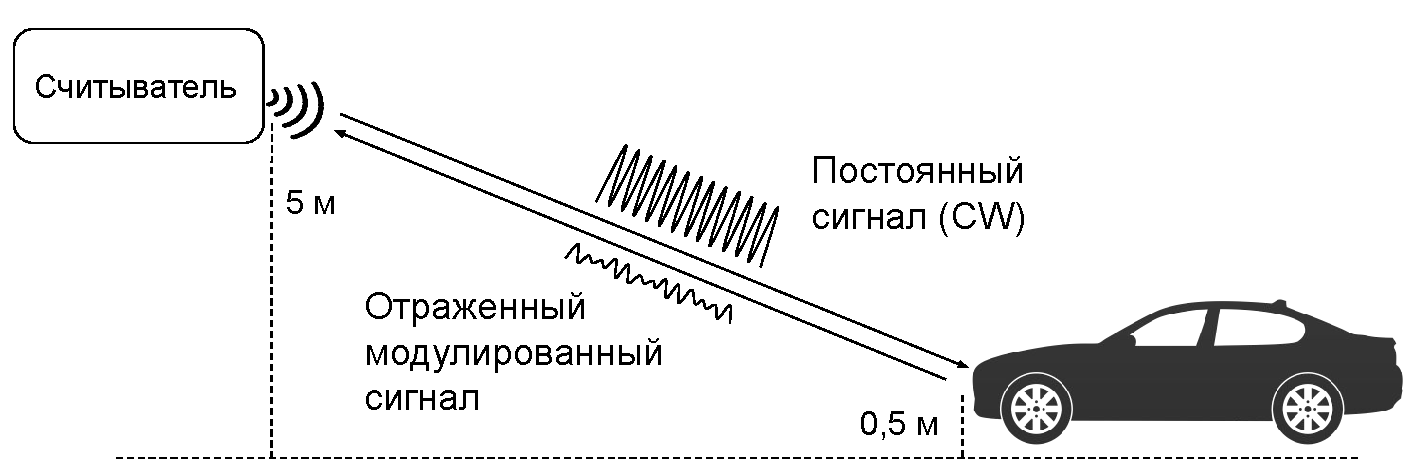
\includegraphics [scale=0.5] {chapter2/ch2_system_structure}
  }
  \caption{Структура системы радиочастотной идентификации автомобилей}
  \label{fig:ch2_system_structure}
\end{figure}

Метки могут размещаться на регистрационных номерных знаках, под лобовым стеклом или на корпусе автомобиля. В настоящей работе рассматривается случай, когда метки расположены на номерах, поскольку этот вариант был использован в проведенном в г. Казань эксперименте. Кроме того, размещение меток в номерных знаках обладает рядом преимуществ: расположение знаков относительно дорожного полотна варьируется в малых пределах, зона номерного знака не загорожена никакими проводящими поверхностями, наконец это решение можно в дальнейшем легко стандартизировать и масштабировать за счет монтирования меток в выпускаемые номерные знаки.

RFID-считыватель размещается над дорогой (например, на тех же опорах, на которых сегодня размещаются камеры), на высоте приблизительно 5 метров; считыватель может оснащаться от 1 до 4 антенн. Таким образом, один считыватель может читать метки в передних и задних номерах на двухполосной дороге.

Связь между меткой и считывателем возможна при соблюдении двух условий: метка получает достаточно энергии для работы и декодирования команд от считывателя (чувствительность современных меток имеет порядок -18 дБм), и отраженный модулированный меткой сигнал поступает на считыватель на достаточно высокой мощности, чтобы быть успешно распознанным и декодированным (при отсутствии коллизий, уровень принимаемого сигнала для современных считывателей должен быть не ниже минус 80 дБм). На практике это означает, что дальность связи составляет порядка 8 -- 15 метров. Однако, из-за особенностей распространения сигнала вблизи автодороги, область, в которой метка может получить достаточно энергии, может иметь достаточно сложный вид и состоять из нескольких непересекающихся областей, общая ширина которых может составлять 2 -- 3 метра. Подробнее эти эффекты будут рассмотрены в последующих разделах.



%%%%%%%%%%%%%%%%%%%%%%%%%%%%%%%%%%%%%%%%%%%%%%%%%%%%%%%%%%%%%%%%%%%%%%%%%%%%%%%%
\section{Общая схема расчёта вероятности идентификации автомобилей}\label{sec:ch2_general_scheme}
%%%%%%%%%%%%%%%%%%%%%%%%%%%%%%%%%%%%%%%%%%%%%%%%%%%%%%%%%%%%%%%%%%%%%%%%%%%%%%%%
Производительность системы определяется как доля успешно идентифицированных автомобилей. Полагая, что успешного чтения хотя бы одной метки достаточно для идентификации автомобиля, вероятность идентификации можно описать следующим образом:

$$
	\mathbb{P}\{A_x\} = 1 - \prod\limits_{\forall t \in  \mathfrak{T}_x} (1 - \mathbb{P}\{A_t\}),
$$
где $A_x$ "--- событие идентификации автомобиля $x$, $A_t$ "--- событие идентификации метки $t$, а $\mathfrak{T}_x$ есть множество меток, размещенных на автомобиле $x$. Вероятность идентификации метки $\mathbb{P}\{A_t\}$ зависит от длительности раунда инвентаризации, вероятности успешной передачи ответа и числа меток в области чтения:

$$
	\mathbb{P}\{A_t\} = 1 - (1 - (1 - \mathbb{P}\{A_c\})\mathbb{P}\{A_r\})^{N_r},
$$
где $A_c$ "--- событие возникновения коллизии, $A_r$ "--- событие успешной передачи меткой ее идентификатора и $N_r$ "--- число раундов, в которых метка успевает принять участие. 

Пусть $N_t$ "--- число меток в области чтения и $Q$ "--- параметр антиколлизионного протокола. \cite{StdGen2}. Тогда вероятность возникновения коллизии для данной метки определяется следующей формулой: 

$$
	\mathbb{P}\{A_c\} = 1 - (1 - 2^{-Q})^{|N_t| - 1}.
$$

Число раундов можно грубо оценить как:

$$
	N_r \approx \frac{D_r}{v}\cdot\frac{1}{T_r},
$$
где $D_r$ "--- общая длина участка дороги с хорошими условиями для чтения (т.е. на этом участке метка получает достаточно энергии для работы и битовая ошибка достаточно низка), $T_r$ "--- средняя длина раунда при заданном числе меток и параметрах протокола, $v$ "--- скорость движения метки. В действительности количество раундов представлеяет собой случайную величину, зависящую от множества параметров, включая количество меток в области чтения, настройки протокола, непосредственный выбор метками слотов для ответов (определяет количество коллизий, пустых слотов и слотов с ответами). Также число раундов зависит от результатов попыток передачи меткой её идентификатора, а также от того, сбрасывал ли считыватель питание между раундами "--- влияние этих факторов оказывается очень существенным и исследуется подробнее в следующей главе диссертации. 

Согласно \cite{Nikitin2008}, при отсутствии коллизий основным источником ошибок при расчете $\mathbb{P}\{A_r\}$ является высокий BER при приеме ответов от меток. Пусть $r$ "--- ответ метки, $\mathfrak{R}$ "--- множество всех ответов метки, передача которых необходима для успешной идентификации. Обозначая битовую длину ответа как $|r|$, вероятность успешной передачи всех ответов $\mathbb{P}\{A_r\}$ метки можно вычислить по формуле:

$$
	\mathbb{P}\{A_r\}=\prod_{r \in \mathfrak{R}}(1-B)^{|r|}.
$$

Множество $\mathfrak{R}$ обязательно содержит ответ RN16 на команду, с которой начался слот, в котором метка передаёт ответ (Query, QueryRep или QueryAdjust) и ответ на команду ACK (PC+EPC+CRC). Если для идентификации метки также используется 64-битное значение из банка TID, то $\mathfrak{R}$ также включает ответы на Req\_RN и Read.

Из приведенных формул видно, что для максимизации вероятности идентификации автомобиля необходимо увеличивать вероятность успешной передачи меткой ответов и число раундов, и одновременно уменьшать вероятность коллизий. Однако эти требования вступают в противоречие: более низкий BER достигается при более надежных и медленных настройках протокола, а вероятность коллизии снижается при росте числа слотов, но все это ведет к увеличению длительности раунда. В последующих разделах будет разработан комплекс моделей, позволяющий проанализировать вероятность идентификации метки при различных допущениях, а в конце главы будут приведены результаты расчета вероятности идентификации автомобиля при различных настройках протокола и скорости движения, полученные с помощью детализированной имитационной модели.







%%%%%%%%%%%%%%%%%%%%%%%%%%%%%%%%%%%%%%%%%%%%%%%%%%%%%%%%%%%%%%%%%%%%%%%%%%%%%%%%
\section{Анализ влияния параметров протокола на длительности раундов}\label{sec:ch2_durations}
%%%%%%%%%%%%%%%%%%%%%%%%%%%%%%%%%%%%%%%%%%%%%%%%%%%%%%%%%%%%%%%%%%%%%%%%%%%%%%%%
Считыватель использует модуляции DSB-ASK, SSB-ASK и PR-ASK, а в качестве схемы кодирования используется PIE. Из-за использования PIE (Pulse Interval Encoding) длительность передачи команды зависит от её содержания, так как длительности символов data\_0 и data\_1 отличаются в 1,5--2 раза. Перед каждой командой Query считыватель передает преамбулу, а перед остальными "--- более короткую синхронизирующую последовательность. В таблице \ref{table:ch2_commands_and_replies_durations} показаны длительности команд и ответов для некоторых настроек протокола. Параметры Tari, TRcal, QUERY и PC+EPC+CRC заданы в микросекундах, BLF "--- в килогерцах, а M выражает число символов на бит в ответе метки (порядок кода Миллера, используемого меткой).

\begin{table}[!t]
	\renewcommand{\arraystretch}{1.3}
	\caption{Длительности команд и ответов при разных настройках протокола.
	Длительности QUERY and PC+EPC+CRC даны в микросекундах.}
	\label{table:ch2_commands_and_replies_durations}
	\centering
	\begin{tabular}{|c|c|c|c|c|c|c|}
		\hline
		DR   & Tari & TRcal & BLF   & M & QUERY & PC+EPC+CRC  \\\hline
		64/3 & 6.25 & 33.38 & 639.2 & 1 & 252.13 & 211.2      \\\hline
		64/3 & 6.25 & 33.38 & 639.2 & 8 & 270.88 & 1739.67    \\\hline
		64/3 & 12.5 & 66.75 & 319.6 & 1 & 491.75 & 422.4      \\\hline
		64/3 & 25.0 & 133.5 & 159.8 & 1 & 971.0  & 844.8      \\\hline
		64/3 & 25.0 & 225.0 & 94.81 & 1 & 1062.5 & 1423.83    \\\hline
		8    & 6.25 & 33.38 & 239.7 & 1 & 245.8  & 563.2      \\\hline
		8    & 25.0 & 225.0 & 33.56 & 8 & 1112.5 & 31275.0    \\\hline
	\end{tabular}
\end{table}

\begin{figure}[!t]
  \centerfloat{
    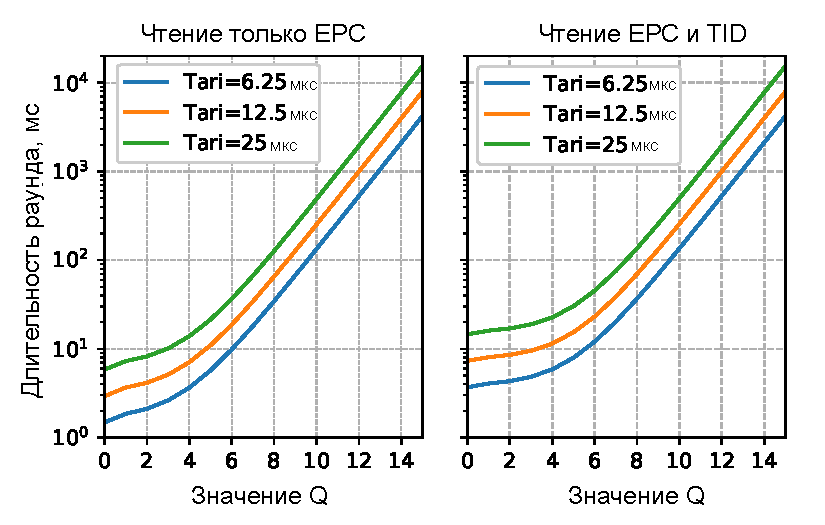
\includegraphics[width=3.3in]{chapter2/ch2_round_durations}
  }
	\caption{Зависимость максимальной длительности раунда от значения Q.}
	\label{fig:ch2_round_durations}
\end{figure}

\begin{figure}[!t]
	\centerfloat{
    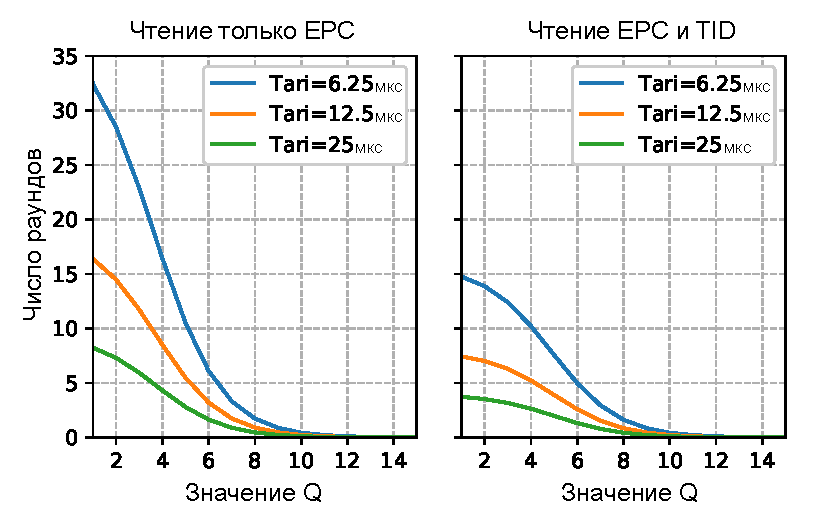
\includegraphics[width=3.3in]{chapter2/ch2_round_numbers}
  }
	\caption{Зависимость максимального числа раундов, в которых принимает участние метка, от значения Q.}
	\label{fig:ch2_round_numbers}
\end{figure}


Выбор значений DR, Tari, M и TRcal значительно влияет на длительности команд и ответов. Так, длительность команды Query может варьироваться от 200~мкс до 1,1~мс, а длительность ответа PC+EPC+CRC на команду ACK "--- от 211~мкс до 31,2~мс (см. табл.~\ref{table:ch2_commands_and_replies_durations}).

При идентификации метки может использоваться только EPCID или комбинация EPCID и значений из других банков, например "--- TID. Первый вариант менее надежен, однако существенно быстрее второго "--- на чтение банков памяти требуется значительно больше времени, так как при этом необходимо осуществить дополнительный обмен сообщениями. На длительность идентификации также влияет, например, использование команды Select для настройки флагов меток и выбора популяции для опроса. В дальнейшем будем рассматривать два самых простых сценария: идентификацию меток только по EPCID (в этом случае взаимодействие ограничивается инвентаризацией) и по комбинации EPCID + TID. Кроме того, будем предполагать, что считыватель не использует команды QueryAdjust и не изменяет выбранное значение параметра Q.

На рис.~\ref{fig:ch2_round_durations} показана максимальная длительность раунда от значения Q, а на рис.~\ref{fig:ch2_round_numbers} "--- максимальное число раундов. Необходимо отметить, что реальная длина раунда может существенно отличаться в зависимости от того, сколько меток в нем отвечает успешно, сколько коллизий происходит и сколько слотов остаются пустыми. Однако, приведенные графики дают возможность увидеть различие в длительностях при использовании разных способов идентификации, а также зависимость от некоторых важных параметров протокола.









%%%%%%%%%%%%%%%%%%%%%%%%%%%%%%%%%%%%%%%%%%%%%%%%%%%%%%%%%%%%%%%%%%%%%%%%%%%%%%%%
\section{Моделирование радиоканала между считывателем и меткой}\label{sec:ch2_channel}
%%%%%%%%%%%%%%%%%%%%%%%%%%%%%%%%%%%%%%%%%%%%%%%%%%%%%%%%%%%%%%%%%%%%%%%%%%%%%%%%
Для передачи данных от метки используется модуляция обратного рассеяния, метка (не оснащенная источником питания) не может усилить отраженный сигнал. Из-за этого мощность сигнала, принятого на стороне считывателя, значительно ниже, чем мощность на стороне метки. По этой причине битовая ошибка (BER) оказывается выше на стороне считывателя, то есть ошибки с гораздо большей вероятностью появляются при приеме ответов от метки, чем команд от считывателя. Значение BER на стороне считывателя оказывает существенное влияние на успешность чтения меток, поэтому это значение должно быть аккуратно рассчитано.

Для анализа BER рассчитаем бюджет соединения и полуичм значение сигнал--шум (SNR). Результаты этого расчета для стационарного считывателя и метки, размещенной на переднем номере автомобиля, двигающегося со скоростью 60~км/ч, приведены на рис.~\ref{fig:ch2_link_budget}. На горизонтальной оси всех графиков показано расстояние между передатчиком и приемником, на вертикальной "--- время, прошедшее с момента достижения волной приемника. Как будет показано далее (см. формулу~\eqref{eq:ch2_pathloss} для вычисления потерь на распространении сигнала), выбор значения скорости движения существенно влияет на скорость изменения величины затухания в заданной точке.

\begin{figure}[!t]
  \centerfloat{
    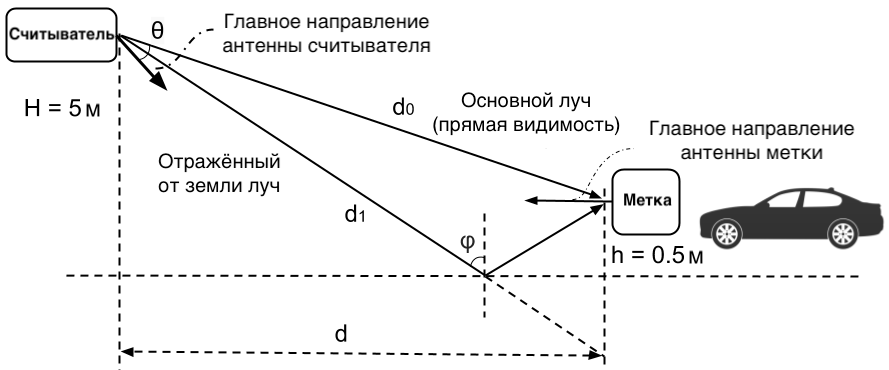
\includegraphics[width=\linewidth]{chapter2/ch2_geometry}
  }
	\caption{Схема системы радиочастотной идентификации автомобилей и ее геометрические параметры.}
	\label{fig:ch2_geometry}
\end{figure}



%%% --------------------------------------------
\subsection{Расчёт бюджета соединений}
%%% --------------------------------------------
Пусть $P_t^{(r)}$ "--- излучаемая мощность считывателя, $G^{(r)}$ "--- усиление антенны считывателя. Тогда эффективная изотропная излучаемая мощность (EIRP) составит $EIRP =  P_t^{(r)} G^{(r)}$. Здесь и далее надстрочный индекс используется для обозначения устройства: (r) для считывателя и (t) для метки; подстрочный индекс используется для обозначения направления передачи (прием или передача сигнала). При распространении сигнала от считывателя к метке сигнал испытывает затухание $A_{pl}^{(d)}$, зависящее от состояния радиоканала и взаимного расположения считывателя и метки друг относительно друга. Антенны устройств могут иметь различную поляризацию, что ведет к дополнительным потерям $A_{pol}$. Пусть усиление антенны метки равно $G^{(t)}$. Тогда мощность сигнала, принимаемого меткой, равна:

$$
	P_r^{(t)} = P_t^{(r)} G^{(r)} A_{pl}^{(d)} A_{pol} G^{(t)}.
$$

Если эта мощность меньше чувствительности метки $P_s^{(t)}$, то метка не включится и не сможет взаимодействовать со считывателем. В противном случае метка сможет передавать свои ответы за счет модулирования отраженного сигнала, мощность которого будет равна $P_t^{(t)}$. Поскольку при этом возникают дополнительные энергетические потери (например, из-за модуляции), равные $A_{bs}$, то мощность принятого и отраженного сигналов связаны как $P_t^{(t)} = P_r^{(t)} + A_{bs}$. 

Для мощности сигнала, принятого от метки считывателем, можно написать следующее соотношение:

$$
	P_r^{(r)} = P_r^{(t)} G^{(t)} A_{bs} A_{pl}^{(r)} A_{pol} G^{(r)}.
$$

В общем случае потери на прямом (от считывателя к метке) и обратном (от метки к считывателю) путях могут отличаться. Это происходит из-за различия в поляризации (обычно на считывателях используются антенны с круговой поляризацией, а на метках "--- с линейной) и, как следствие, в коэффициенте отражения от земли.

\begin{table}[!t]
	\renewcommand{\arraystretch}{1.3}
	\caption{Параметры, использованные при расчете бюджета соединения}
	\label{table:ch2_budget_params}
	\centering
	\begin{tabular}{|c|c|}
		\hline
		Мощность, излучаемая считывателем, $P_t^{(r)}$ & 31.5~дБм\\
		\hline
		Усиление антенны считывателя, $G^{(r)}$ & 8~дБи\\
		\hline
		Усиление антенны метки, $G^{(t)}$ & 2~дБи\\
		\hline
		Чувствительность метки, $P_s^{(t)}$ & -18~дБм\\
		\hline
		Потери на поляризации, $A_{pol}$ & -3~дБ\\
		\hline
		Потери на модуляции на метке, $A_{bs}$ & -10~дБ\\
		\hline
		Потери в кабеле, $A_{bs}$ & -2~дБ\\
		\hline
	\end{tabular}
\end{table}

В дальнейших расчетах бюджета соединения будут использованы значения, приведенные в таблице~\ref{table:ch2_budget_params}, типичные для оборудования, применяемого в идентификации автомобилей. При расчете также следует учитывать потери в кабеле, соединяющем антенну со считывателем. Далее считается, что антенны считывателя имеют круговую поляризацию, а меток "--- линейную, таким образом потери на поляризации составляют -3~дБ.

\begin{figure}[!t]
	\centerfloat{
    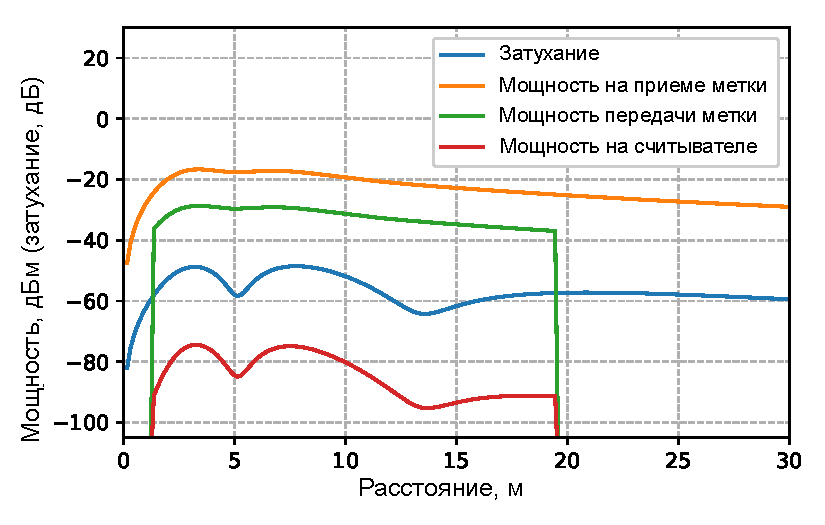
\includegraphics[width=3.3in]{chapter2/ch2_link_budget}
  }
  \caption{Расчет бюджета соединения в зависимости от расстояния между считывателем и меткой.}
  \label{fig:ch2_link_budget}
\end{figure}

На рис.~\ref{fig:ch2_link_budget} показан расчет мощностей сигналов, принятых и переданных меткой, принятого считывателем сигнала, а также величина затухания. Все кривые убывают немонотонно из-за изменений с расстоянием в коэффициентах отражения от земли, а также из-за влияния диаграмм направленности антенн (особенно сильно диаграмма направленности влияет на сигнал при близком расположении метки и считывателя, так как даже небольшое изменение расстояния ведет к ощутимому изменению в угле падения). Поскольку метка может работать только в тех областях, где принятый ею сигнал превышает чувствительность, графики мощностей передаваемого меткой и принимаемого считывателем сигнала лежат выше нуля только на ограниченном интервале.

На рис.~\ref{fig:ch2_heatmap_pathloss} показана величина потери из-за затухания сигнала при распространении от считывателя к метке (картина для обратного канала отличается незначительно), а на рис.~\ref{fig:ch2_heatmap_tag_rx_power} показан результат расчета мощности сигнала, принятого меткой. Для того, чтобы связь между расстоянием от считывателя до метки и временем при постоянной скорости оставалась линейной, в качестве расстояния рассматривается дистанция от опоры, на которой размещен считыватель, до метки, измеренная вдоль дороги (см. величину $d$ на рис.~\ref{fig:ch2_geometry}). Значительное влияние на результат расчета оказывает эффект Доплера, подробнее о котором будет рассказано в следующем разделе. Фактически из-за этого эффекта канал становится зависимым от времени, то есть при проезде через одну и ту же точку двух одинаковых меток в разное время принятая ими (а, соответственно, и отраженная) мощность будет различаться.


%    \centerfloat{
%        \hfill
%        \subcaptionbox[List-of-Figures entry]{Первый подрисунок\label{fig:knuth_2-1}}{%
%            \includegraphics[width=0.25\linewidth]{knuth1}}
%        \hfill
%        \subcaptionbox{\label{fig:knuth_2-2}}{%
%            \includegraphics[width=0.25\linewidth]{knuth2}}
%        \hfill
%        \subcaptionbox{Третий подрисунок, подпись к которому
%        не~помещается на~одной строке}{%
%            \includegraphics[width=0.3\linewidth]{example-image-c}}
%        \hfill
%    }
%    \legend{Подрисуночный текст, описывающий обозначения, например. Согласно
%    ГОСТ 2.105, пункт 4.3.1, располагается перед наименованием рисунка.}
%    \caption[Этот текст попадает в названия рисунков в списке рисунков]{Очень
%    длинная подпись к второму изображению, на~котором представлены две
%    фотографии Дональда Кнута}\label{fig:knuth_2}

\begin{figure}[ht]
  \centerfloat{
    \hfill
    \subcaptionbox{Затухание сигнала при распространении от считывателя к метке, дБ\label{fig:ch2_heatmap_pathloss}}{%
      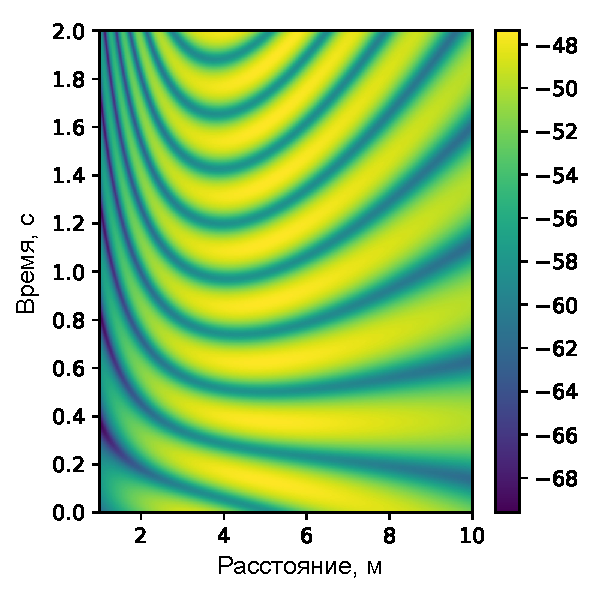
\includegraphics[width=0.30\linewidth]{chapter2/ch2_heatmap_pathloss}
    }
    \hfill
    \subcaptionbox{Мощность принятого на метке сигнала, дБм\label{fig:ch2_heatmap_tag_rx_power}}{%
      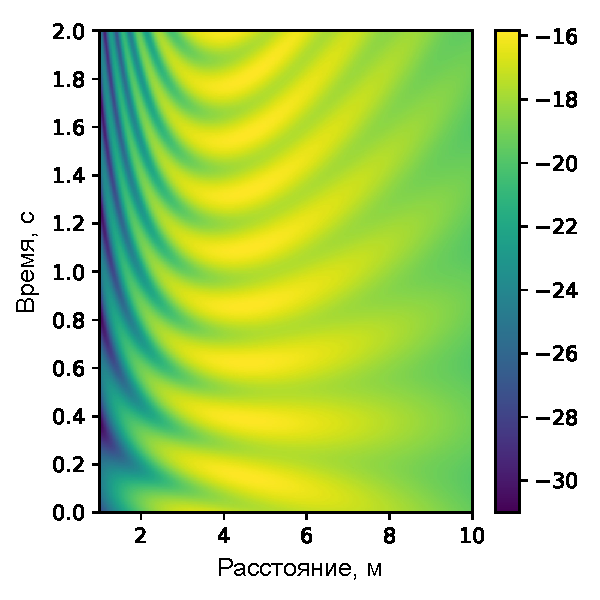
\includegraphics[width=0.30\linewidth]{chapter2/ch2_heatmap_tag_rx_power}
    }
    \hfill
    \subcaptionbox{Битовая ошибка (BER) на считывателе\label{fig:ch2_heatmap_ber}}{%
      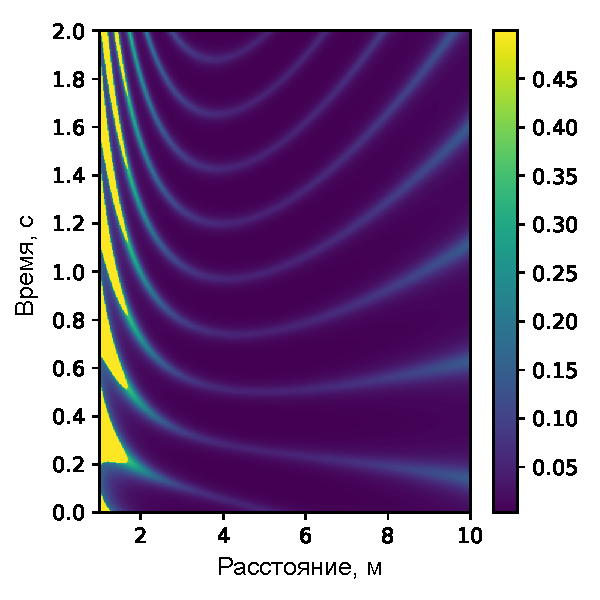
\includegraphics[width=0.30\linewidth]{chapter2/ch2_heatmap_ber}
    }
  }
  \legend{На горизонтальных осях показано расстояние от точки крепления считывателя до метки вдоль дороги (см. величину $d$ на рис.~\ref{fig:ch2_geometry}). На вертикальных осях показано время от начала приема меткой сигнала. Из-за эффекта Доплера канал меняется со временем, т.е. метки, расположенные на автомобилях, проезжающих через одну и ту же точку в разное время, застают канал в разных состояниях и получают сигналы разной мощности.}
  \caption{Расчет бюджета соединений и BER}
  \label{fig:ch2_heatmap}
\end{figure}




%%% --------------------------------------------
\subsection{Расчёт мощности принятых сигналов}
%%% --------------------------------------------

При движении меток и считывателей с ненулевой скоростью друг относительно друга сигналы оказываются подверженными эффекту Доплера, проявляющемуся в сдвиге частоты сигнала на величину, называемую доплеровским сдвигом, и равную:

$$
	\alpha = 1 - \frac{\upsilon \cos{\psi}}{c+\upsilon \cos{\psi}},
$$
где $c$ "--- скорость света, $\upsilon$ "--- скорость приёмника относительно передатчика, в роли приёмника может выступать как метка, так и считыватель (при этом их скорости будут иметь одинаковую величину и противоположные знаки), $\psi$ "--- угол между волновым вектором $\bm{k}$ и направлением движения, $f_c$ "--- несущая частота. 

Для узкополосного сигнала в RFID-канале смещённую частоту можно приблизить выражением $\alpha f \approx f - \frac{\upsilon}{c}\cos{\psi} \cdot f_c = f - \nu$, где $\nu$ "--- доплеровский сдвиг:

$$
	\nu = \frac{\upsilon}{c} f_c\cos{\psi} = \frac{1}{2\pi}(\bm{\upsilon},\bm{k})
$$

При распространении сигнала он может отражаться от дороги, инженерных конструкций, других автомобилей и прочих объектов, то есть в моделируемой системе имеет место многолучевое распространение сигнала. При этом возникает множество копий сигнала $s(t)$, каждая из которых испытывает собственное затухание $h_i$, задержку $\tau_i$ и доплеровский сдвиг $\nu_i$, поскольку каждая копия распространяется по собственному пути, с которым, помимо длины, связаны углы передачи и приема сигнала. Пусть в сигнале присутствует прямая компонента (Line-of-Sight, LoS) сигнала и $N$ отраженных компонент (или лучей). Без потери общности рассуждений будем считать, что LoS-компонента описывается нулевым лучём, а отраженные компоненты "--- лучами $1 \dots N$. Принятый сигнал определяется следующей формулой:

\begin{equation}
	r(t) = \sum\limits_{i=0}^{N} h_i s(t-\tau_i) e^{j\nu_i t},
	\label{eq:ch2_rx_signal}
\end{equation}

Затухание $h_i$ может быть рассчитано как $h_i=\lambda/(4\pi d_i)R_i\Gamma_i$, где $\lambda$ "--- длина волны, $d_i$ "--- длина пути для $i$--го луча, $R_i$ "--- коэффициент затухания, вызванного отражением сигнала, для $i$--го луча (для основной, LoS-компоненты полагаем равным единице: $R_0=1$), $\Gamma_i = \Gamma_i^{(r)}\Gamma_i^{(t)}$ "--- ослабление сигнала, определяемое диаграммами направленности передающей и принимающей антенн.

Рассмотрим в качестве передаваемого сигнала постоянную волну (синусоидальный сигнал) единичной мощности. После подстановки формул, описанных выше, в выражение для $r(t)$ \eqref{eq:ch2_rx_signal}, получим затухание при распространении сигнала как значение мгновенной мощности на приемнике: 

\begin{equation}
	A_{pl} = |r(t)|^2 = \left(\frac{\lambda}{4\pi}\right)^2
		\left|\sum\limits_{i=0}^{N} \frac{R_i\Gamma_i}{d_i} 
		e^{-jk(d_i-\upsilon t \cos{\psi_i})}\right|^2
	\label{eq:ch2_pathloss}
\end{equation}

Расчёт $R_i$, $\Gamma_i$, $d_i$ и $\psi_i$ требует определения путей распространения сигнала по разным лучам. Для статического окружения, при пренебрежении отражениями от движущихся автомобилей, пути могут быть вычислены простыми аналитическими методами. При более сложном динамическом окружении (а также при моделировании отражающих объектов сложной формы) потребуется использовать техники трассировки лучей. Далее, для упрощения расчетов, будем учитывать только две компоненты: прямую (LoS) и отраженную от земли (NLoS) компоненты. Для отраженной NLoS-компоненты коэффициент затухания $R_1$ равен коэффициенту отражения от земли. Далее предполагаем, что антенна считывателя размещена на высоте 5~м, а метки "--- 0,5~м над дорогой. Остальные лучи моделируются нявно, как случайные компоненты,  обуславливающие использование распределение Рэлея при вычислении BER (подробнее об этом "--- в следующем подразделе). 

\begin{figure}[!t]
	\centerfloat{
    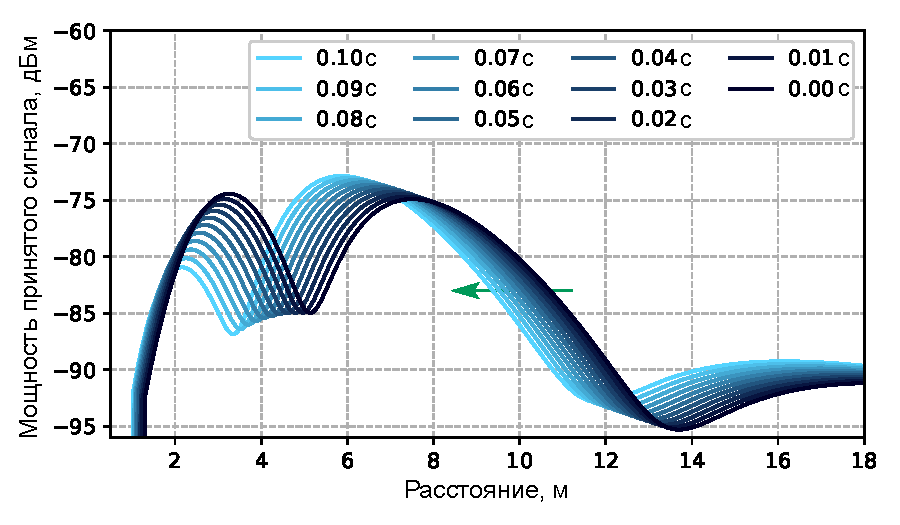
\includegraphics[width=3.3in]{chapter2/ch2_power_doppler}
  }
  \caption[Зависимость мощности сигнала, принятого считывателем, от расстояния и времени]{Зависимость мощности сигнала, принятого считыватлем, от расстояния между считывателем и меткой $d$ и временем, прошедшим с начала приема меткой сигнала от считывателя.}
	\label{fig:ch2_power_doppler}
\end{figure}

\begin{figure}[!t]
	\centerfloat{
    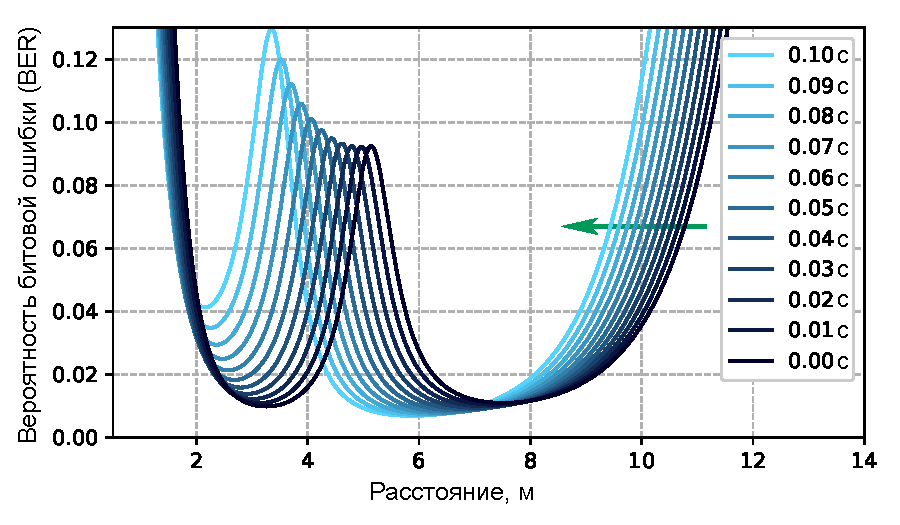
\includegraphics[width=3.3in]{chapter2/ch2_ber_doppler}
  }
	\caption[Зависимость BER от расстояния и времени]{Зависимость вероятности битовой ошибки (BER) от расстояния между считывателем и меткой $d$ и временем, прошедшим с начала приема меткой сигнала от считывателя.}
	\label{fig:ch2_ber_doppler}
\end{figure}



Наличие эффекта Доплера делает канал зависимым от времени (см. \cite{Matz2011}), поскольку, как видно из формулы \eqref{eq:ch2_rx_signal}, величина сдвига для каждого луча определяется индивидуально и зависит от времени, прошедшего с начала получения сигнала. Особенность RFID-системы состоит в том, что считыватель не перестает передавать сигнал (постоянный, который метка может модулировать для передачи своего ответа, или информационный) ни после передачи своей команды, ни после получения ответа. Считыватель может прекращать передачу сигнала, например, для сброса флагов сессий меток, при переключении частот или в том случае, если по законодательству он должен периодически освобождать радиоканал. Однако, такие прерывания происходят относительно редко, внутри одного или нескольких раундов сигнал не прерывается. Поэтому значение $t$ в \eqref{eq:ch2_rx_signal} определяется как время, прошедшее со включения считывателя, за вычетом длительности распространения сигнала от считывателя до метки. Хотя метка в это время может еще находиться далеко, радиоканал уже будет существовать. Учитывая, что в момент включения считывателя метки расположены на разных расстояниях от считывателя, получаем, что значение $t$ в одной и той же точке для разных меток будет разным, а соответственно разными будут и значения $r(t)$. Так, на рис.~\ref{fig:ch2_power_doppler} показана зависимость мощности сигнала, принятой считывателем, от расстояния $d$, измеренного вдоль дороги, а на рис.~\ref{fig:ch2_ber_doppler} "--- зависимость вероятности битовой ошибки (BER) от расстояния $d$. Различные кривиые соответствуют различному времени, прошедшему с начала приема меткой сигнала от считывателя. Графики на рис.~\ref{fig:ch2_heatmap}, \ref{fig:ch2_power_doppler} и \ref{fig:ch2_ber_doppler} показывают, как эффект Доплера делает канал зависимым от времени: области хорошего приема с высоким уровнем принятого сигнала и, соответственно, низким BER, сдвигаются с течением времени. 

\begin{figure}[!t]
	\centerfloat{
    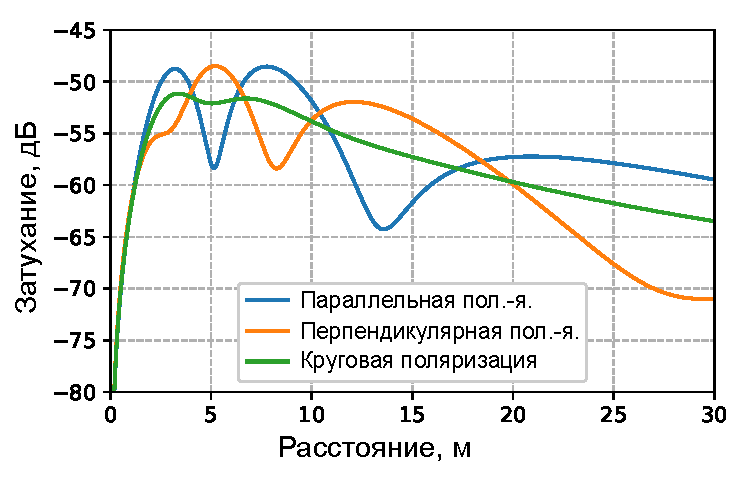
\includegraphics[width=3.3in]{chapter2/ch2_pathloss_cases}
  }
	\caption{Зависимости потери при распространении сигнала от расстояния для параллельной, перпендикулярной и круговой поляризаций. Для круговой поляризации комплекснозначный коэффициент равен полусумме коэффициентов для параллельной и перпендикулярной поляризаций.}
	\label{fig:ch2_pathloss_cases}
\end{figure}

На рис.~\ref{fig:ch2_pathloss_cases} показаны результаты расчета затухания сигнала в зависимости от расстояния для разных видов поляризации: параллельной, перпендикулярной и круговой. Различие обусловлено тем, что коэффициент отражения от земли $R_1$ для NLoS-компоненты сигнала принимает разные значения в зависимости от выбранной поляризации (см. рис.~\ref{fig:ch2_reflection}). 

Коэффициент отражения определен следующей формулой \cite{Gonzalez2013}:
$$
  R = \frac{\sin\phi - \sqrt{C}}{\sin\phi + \sqrt{C}},
$$
где $\phi$ "--- угол падения, $C = \eta - \cos^2\phi$ для горизонтально поляризованной компоненты и $C = \frac{\eta - \cos^2\phi}{\eta^2}$ для вертикально поляризованной; $\eta = \epsilon_r(f)-j60\lambda\sigma(f)$, где $\epsilon_r(f)$ "--- относительная диэлектрическая проницаемость поверхности для заданной частоты $f$, $\sigma(f)$ "--- проводимость.

\begin{figure}[!t]
	\centerfloat{
    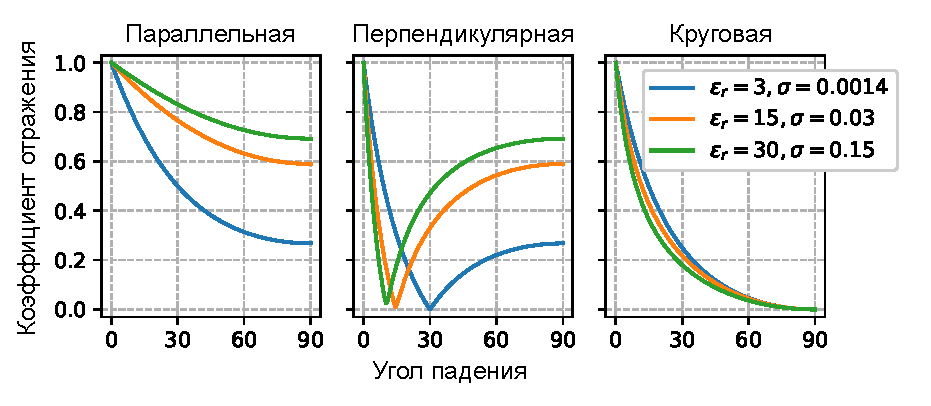
\includegraphics[scale=0.75]{chapter2/ch2_reflection}
  }
	\caption{Зависимость коэффициента отражения от угла падения для параллельной, перпендикулярной и круговой поляризации при разных значениях относительной диэлектрической проницаемости $\epsilon$ и проводимости $\sigma$.}
	\label{fig:ch2_reflection}
\end{figure}

Относительная диэлектрическая проницаемость и проводимость сильно зависят от влажности поверхности. Проводимость меняется в диапазоне от 0.00014~См/м для очень сухой земли до 5~См/м для морской воды. Относительная диэлектрическая проницаемость меняется в диапазоне от 3 до 70. На рис.~\ref{fig:ch2_reflection} показана зависимость коэффициента отражения от угла для разных значений относительной диэлектрической проницаемости $\epsilon$ и проводимости $\sigma$.

Далее будем считать, что у метки простая дипольная антенна, и её диаграмма направленности определяется как:

\begin{equation}\label{eq:ch2_dipole}
	\Gamma(\theta) = \left| 
		\frac{\cos{\frac{\pi}{2}\sin{\theta}}}{\cos{\theta}} \right|,
\end{equation}

Для простоты, будем считать, что диаграмма антенны считывателя также определяется с помощью~\eqref{eq:ch2_dipole}. Для более точного расчета можно использовать более подходящие диаграммы, например "--- патч-антенны \cite{Balanis2016}.




%%% --------------------------------------------
\subsection{Расчёт вероятности битовой ошибки (BER)}
%%% --------------------------------------------
\begin{figure}[!t]
	\centerfloat{
    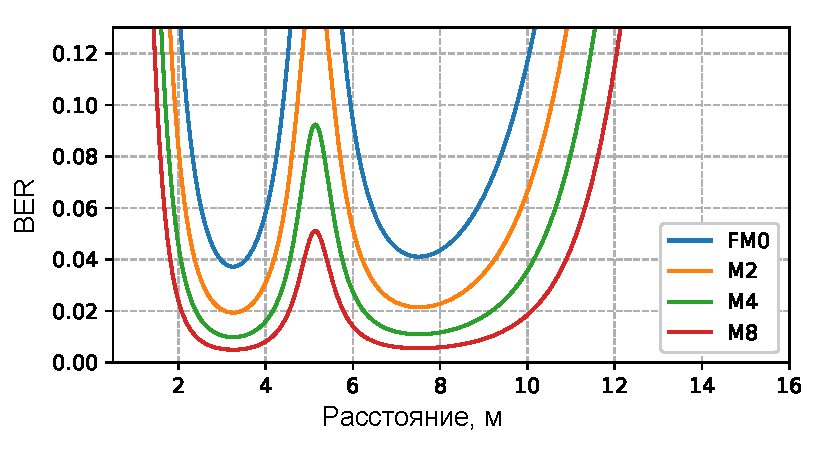
\includegraphics[width=3.3in]{chapter2/ch2_ber_miller}
  }
	\caption{Вероятность битовой ошибки (BER) для разных модуляций ответов метки.}
	\label{fig:ch2_ber_miller}
\end{figure}

Рассмотрим радиоканал с аддитивным гауссовским шумом (AWGN). Вероятность ошибки в передаче бита (BER) можно выразить следующей формулой:

\begin{equation}
	P_{er} = 2Q(\acute{\gamma})[1-Q(\acute{\gamma})],
	\label{eq:ch2_awgn}
\end{equation}
где $Q(\cdot)$ "--- Q--функция; $\acute{\gamma} = mE_s/N_0\cos^2{\phi_s}$; $m$ "--- число символов на бит (порядок) в коде Миллера, $E_s$ "--- энергия одного символа, $N_0/2$ "--- спектральная плотность белого шума и $\phi_s$ "--- разность между реальной и принятой фазами сигнала. Соотношение $E_s/N_0$ может быть выражено как $\gamma T_s B$, где $\gamma$ отношение сигнал-шум (SNR), $T_s$ "--- длительность символа и $B$ "--- ширина полосы.

Для синхронизации фазы передатчик начинает передачу кадра с преамбулы. Ошибка в оценке этой фазы выражается параметром $\phi_s$, который может быть промоделирован с помощью нормально распределенной случайной величины с нулевым средним и дисперсией $\sigma_s^2 = 1/\gamma T_{pr}B$, где $T_{pr}$ "--- длительность преамбулы.

Использование гауссовской модели оказывается слишком оптимистичным, так как при расчете мощности принятого сигнала учитываются не все лучи. Поэтому далее будет использоваться выражением, получаемым усреднением $P_{er}$ в формуле \eqref{eq:ch2_awgn} по $\acute{\gamma}$, которую считаем случайной величиной, имеющей распределение Рэлея \cite{Lazaro2009}:

$$
	P_{er} = \frac{1}{2} - \frac{1}{\sqrt{1+\frac{2}{\acute{\gamma}}}} +
			 \frac{2}{\pi}\frac{\arctan{\sqrt{1+\frac{2}{\acute{\gamma}}}}}{1+\frac{2}{\acute{\gamma}}}.
$$

На рис.~\ref{fig:ch2_ber_miller} показана зависимость BER от выбранного типа кодирования ответа метки. Как и следовало ожидать, при росте числа символов на бит $m$ BER снижается. Влияние эффекта Доплера на BER показано на рис.~\ref{fig:ch2_ber_doppler} и рис.~\ref{fig:ch2_heatmap_ber}. Из-за высокого BER (0.02 и выше) на большей части дороги успешный прием данных от метки практически невозможен, таким образом для передачи данных остаются небольшие <<окна>> шириной 1--2 метра, в которых BER оказывается достаточно низок.







%%%%%%%%%%%%%%%%%%%%%%%%%%%%%%%%%%%%%%%%%%%%%%%%%%%%%%%%%%%%%%%%%%%%%%%%%%%%%%%%
\section{Имитационная модель}\label{sec:ch2_sim}
%%%%%%%%%%%%%%%%%%%%%%%%%%%%%%%%%%%%%%%%%%%%%%%%%%%%%%%%%%%%%%%%%%%%%%%%%%%%%%%%
Для анализа системы радиочастотной идентификации была разработана имитационная модель, позволяющая анализировать производительность системы при разных настройках протокола, учитывающая особенности окружения и интенсивность автомобильного трафика. Имитационная модель позволяет учитывать многолучевое распространение сигнала, эффект Доплера, диаграммы направленности антенн и прочие особенности, описанные ранее. Также имитационная модель содержит детализированную реализацию протокола EPC Gen2, позволяя оценивать производительность системы в зависимости от всевозможных настроек протокола, включая длительности символов, схемы кодирования ответов меток, сценарии управления питанием считывателя и прочее. Модель реализована на языке Python 3. Исходный код и документация доступны на GitHub по адресу https://github.com/larioandr/thesis-models/src/rfidsim.



%%% --------------------------------------------
\subsection{Библиотека дискретно-событийного моделированя PyONS}
%%% --------------------------------------------
Специально для имитационной модели системы радиочастотной идентификации на языке Python 3 была разработана экспериментальная библиотека для дискретно-событийного моделирования PyONS. Исходный код и документация также доступны на GitHub по адресу https://github.com/larioandr/thesis-models/src/pyons. При разработке ставились следующие задачи:

\begin{itemize}
\item возможность написания моделей в функциональном или объектно-ориентированном стиле;
\item обработчики событий, инициализаторы и финализаторы, условия остановки и удаления объектов "--- произвольные функции или методы Python со специальными декораторами;
\item диспетчеризация событий "--- через предикаты, задаваемые в декораторах обработчиков;
\item модели должны содержать минимум <<ритуального кода>>, то есть связывания обработчиков и событий, выполнение инициализаторов и финализаторов и прочие служебные действия должны происходить внутри системы моделирования, и не должны требовать дополнительных вызовов из самих моделей.
\end{itemize}

Состояние системы можно определять либо с помощью произвольного объекта (например, словаря \texttt{dict} или класса данных \texttt{dataclass}), либо с помощью специальных объектов (\textit{сущностей}), унаследованных от класса \texttt{Entity}. В первом случае все управляющие функции задаются с помощью обычных функций Python. Сама модель устанавливается вызовом \texttt{set\_model()} перед началом симуляции и может быть получена из любого обработчика вызовом функции \texttt{get\_model()}. Во втором случае управляющие функции могут также задаваться функциями, но можно их также определять как методы объекта-сущности. После создания, сущности нужно регистрировать в симуляторе вызовом \texttt{add\_entity()}. В любом случае, функции или методы, выполняющие управление моделью, должны снабжаться специальными декораторами.

Сущности модели имеют свой жизненный цикл. После создания они инициализируются, для чего выполняются все методы-инициализаторы, которые в них определены. Затем сущности могут обрабатывать события, пока один из их методов, помеченных как <<условие смерти>>, не вернет \texttt{True}. Если это произойдет, будут выполнены все методы, помеченные как финализаторы, и после этого сущность будет удалена, а все события, которые предназначались ей или отправлены ею, но еще не обработаны, будут отменены. Использование сущностей

Система определяет шесть типов управляющих функций или методов, для которых используются специальные декораторы:

\begin{itemize}
\item \texttt{eventhandler(guard, default, name)} "--- декоратор для обработчиков событий, в который передается предикат (\texttt{guard}), возвращающий True, если событие должно обрабатываться этим обработчиком. Один из обработчиков может быть определен с декоратором, в котором \texttt{default = True}, он будет вызываться, если предикаты всех обработчиков вернули \texttt{False}. Обработчику можно задать удобно читаемое имя (последний параметр декоратора).
\item \texttt{initializer(stage, name)} "--- декоратор для функций или методов, инициализирующих модель. Первый параметр определяет порядок вызова инициализаторов, если их несколько. Смысл инициализатора-функции и инициализатора-метода разный: функция вызывается в начале запуска модели, а метод "--- при создании объекта-сущности.
\item \texttt{finalizer(stage, name)} "--- декоратор для функций, выполняющихся в конце симуляции, или методов, которые выполняются в случае смерти объекта-сущности.
\item \texttt{stop\_condition(guard, name)} "--- декоратор для функций или методов, которые выполняют роль предиката остановки: если одна из таких функций вернет \texttt{True}, симуляция будет остановлена. Для экономии времени, предикаты остановки выполняются не всегда, а только когда функция \texttt{guard} (\textit{страж}, первый аргумент декоратора) возвращает \texttt{True}. Следует отметить, что страж имеет смысл определять только тогда, когда его выполнение занимает меньше времени, чем проверка самого условия остановки.
\item \texttt{death\_condition(guard, name)} "--- декоратор для методов, выполняющих роль условий гибели сущности. Если один из таких методов объекта-сущности вернет \texttt{True}, то сущность погибнет "--- выполнятся все ее методы-финализаторы и она будет удалена из системы. Роль первого аргумента (стража) аналогична его роли в декораторе условий остановки \texttt{stop\_condition(guard, name)}. Условием смерти может быть только метод класса-сущности, для функций вне сущностей он не имеет смысла.
\item \texttt{managed} "--- декоратор без аргументов для методов сущностей. Он не выполняет специфических задач, но его вызов попадает в стек модели.
\end{itemize}

Так как события связываются с обработчиками с помощью предикатов, то код моделей можно организовать по-разному. Например, можно использовать единственную функцию-обработчик в каждой сущности, без предиката-сторожа (\texttt{guard = None}) и установленную по-умолчанию (\texttt{default = True}). Такой же подход используется в OMNeT++, где для обработки событий используется перегружаемая функция \texttt{handleMessage()}. А можно вводить отдельные обработчики для каждого типа событий, и с помощью предикатов определять связи между конкретными событиями и обработчиками.

Система моделирования поддерживает свой собственный стек вызовов, в который попадают управляющие функции и методы. Это позволяет, например, однозначно идентифицировать объект-сущность, метод которого в данный момент выполняется. Это необходимо при создании новых событий, так как в них хранится информация о том, какой обработчик какой сущности это событие создал. Эта информации очень часто нужна для диспетчеризации "--- выбора обработчика для события. Например, событие окончания ожидания ответа должно обрабатывать та же метка, которая его создала.

В ядре модели определно две очереди: очередь будущих запланированных событий и очередь мгновенных вызовов. В качестве очереди будущих событий используется стандартная куча (heap queue) с упорядочиванием по времени наступления событий и, если времена одинаковы, их идентификаторам. Для событий, которые должны наступить в настоящем (то есть фактически для вызова функций-обработчиков, но не из контекста текущего обработчика) используется отдельный массив, чтобы снизить нагрузку на очередь отложенных событий, так как добавление и извлечение событий из нее требует больше времени ($O(1)$ против $O(\log N)$).

Событием в имитационной модели может быть что угодно, включая строки, кортежи, числа, произвольные объекты. Вместе с каждым событием хранятся: его идентификатор, сущность назначения (\texttt{target}, необязательное поле), сущность, которая создала событие (\texttt{source}, необязательное поле) и время наступления события (\texttt{fire\_time}). Для работы с событиями определены три функции:

\begin{itemize}
\item \texttt{create\_timeout(dt, event)} "--- создать событие-таймаут, которое должно наступить через интервал \texttt{dt}, для той же сущности, которая его создает. Если создание происходит не из некоторого метода объекта-сущности, то сущность назначения не будет определена. События, созданные с помощью этого вызова, попадают в очередь будущих событий.
\item \texttt{send\_event(event, entity)} "--- создать событие, которое должно быть обработано указанной сущностью. Это событие попадет в очередь мгновенных событий (то есть массив). Использование \texttt{send\_event} медленнее, чем простой вызов метода объекта-сущности. Однако, во-первых, оно позволяет не указывать явно, какой именно метод нужно вызывать и, во-вторых, вызов соответствующего метода-обработчика произойдет уже после того, как вызывающий обработчик полностью завершится.
\item \texttt{cancel(event\_id)} "--- удалить запланированное, но еще не обработанное событие с заданным идентификатором. Идентификатор возвращается функциями \texttt{create\_timeout()} и \texttt{send\_event()}.
\end{itemize}

Для того, чтобы ядро могло вызывать инициализаторы и финализаторы, находить обработчики событий и проверять условия остановки или смерти сущностей, оно должно знать о них. Декораторы управляющих функций регистрируют их в специальном реестре статических функций \texttt{StaticRegistry}. Так как декораторы выполняются при импорте модуля, то для этого достаточно импортировать файл, в котором определены функции, в модуль, содержащий функцию, вызывающую выполнение модели. Для класса \texttt{StaticRegistry} используется шаблон Singleton, то есть в любой момент времени в системе существует ровно один его объект.

С сущностями ситуация сложнее, так как для вызова метода нужно иметь созданный объект класса-сущности. Для решения этой задачи все классы-сущности используют метакласс \texttt{MetaEntity}, в котором определен аналог реестра статических функций. Конструктор метакласса вызывается при определении класса. Он просматривает все атрибуты класса, находит управляющие методы и записывает их в свой реестр. Этот реестр (фактически, набор спиской  для каждого типа управляющих функций) добавляется к атрибутам создаваемого класса, и далее используется для поиска и итераций по управляющим методам. Для созданных объектов-сущностей используется отдельный реестр \texttt{EntitiesRegistry}, в котором хранятся сущности и информация об их состоянии (только создана, инициализирована, готова к удалению).

Более подробную информацию о реализации PyONS и простые примеры моделей можно найти в документации проекта на GitHub. Основное преимущество реализованной системы моделирования - простота написания моделей, поддержка функциональной и объектно-ориентированной парадигмы программирования, высокая гибкость, а также то, что весь код реализован на Python и может легко интегрироваться с популярными библиотеками работы с числовыми данными "--- NumPy, Pandas, SciPy и другими. Главный же недостаток "--- низкая производительность, которая обусловлена как тем, что вся реализация построена на Python, так и тем, что при обработке каждого события происходит выполнение большого количества служебного кода "--- в первую очередь, поиск нужного обработчика, а также проверка условий остановки и смерти. Возможное решение проблемы с производительностью в перспективе "--- переписать часть ядра на C/C++ и использовать Cython.




%%% --------------------------------------------
\subsection{Модель системы радиочастотной идентификации}
%%% --------------------------------------------
Модель системы радиочастотной идентификации автомобилей построена на базе библиотеки PyONS. Некоторые архитектурные идеи при разработке были заимствованы из библиотеки INET системы моделирования OMNeT++, однако реализованы на Python и с существенными упрощениями, адаптированными для модели RFID.

Модель поддерживает следующие параметры: число полос движения и их ширина, стороны расположения антенн считывателя и меток (передние и/или задние номера), учитывать или нет эффект Доплера, модели расчета затуханий и BER, уровень термического шума и шума в циркуляторе, диэлектрическая проницаемость и проводимость дорожного полотна, угол установки антенн считывателя, смещение по горизонтали и высота подвеса антенн считывателя, высота размещения меток, диаграмма, поляризация и усиление антенн, потери на модуляции (для меток), в кабелях (для считывателя), выходная мощность и частота считывателя, интервалы и длительность сброса питания считывателя, частота обновления положений автомобилей с метками, стратегия выбора флагов сессий, число раундов на каждой антенне, значения Tari, TRcal, RTcal, TRext, M, Q, DR, SL, скорость и длина автомобилей, чувствительность меток, интервалы между появлениями и длительность нахождения в системе автомобилей.

Автомобили появляются в системе через заданные интервалы, причем интервал можно задавать как случайную функцию без аргументов, чтобы сильнее рандомизировать результаты. Скорость движения всех автомобилей одинакова, и через заданное время автомобили исчезают из системы.


В модели определены классы-сущности (наследники класса \texttt{pyons.Entity}):

\begin{itemize}
	\item \texttt{Reader} "--- модель считывателя, которая отвечает за логику создания команд и обработки ответов, периодическое включение и выключение питания, циклическую активизцию антенн;
	\item \texttt{Tag} "--- модель метки, отвечает за логику обработки команд и формирование ответов, а также моделирует включения и отключения при изменении мощности принятого сигнала;
	\item \texttt{Vehicle} "--- модель автомобиля, задача которой "--- периодическое обновление положения связанных с ней меток;
	\item \texttt{Generator} "--- генератор автомобилей, периодически добавляет в систему новые машины;
	\item \texttt{Trasceiver} "--- модель трансивера, отвечающая за прием, обработку и передачу сигналов;
	\item \texttt{Signal} "--- модель сигнала с кадром команды или ответа с заданным приемником и отправителем, хранит текущее значение мощности и обрабатывает события начала и окончания приема;
	\item \texttt{Channel} "--- модель радиоканала, использующаяся трансиверами для расчета затуханий сигнала.
\end{itemize}

Кроме классов-сущностей, есть несколько вспомогательных классов, в которых нет обработки событий, но методы которых используются из сущностей: 

\begin{itemize}
	\item \texttt{ReaderDecider}, \texttt{TagDecider} "--- реализуют метод \texttt{decide()}, возвращающий признак того, успешно ли принят сигнал, а также значения максимального BER и минимального SNR. \texttt{TagDecider} возвращает признак успеха, если полученный сигнал был единственным, и он не прерывался, в противном случае сообщает о коллизии. Сигнал на метке считается прерванным, если во время его получения она отключалась из-за снижения мощности ниже порога чувствительности. \texttt{ReaderDecider} также анализирует, был ли сигнал единственным и не прерывался ли он. После этого, если сигнал был непрерывным и он был один, он вычисляет SNR, и по нему находит оценку BER, с помощью которой вычисляет вероятность успешного приема ответа метки. Если случайное число от 0 до 1, оказывается не более, чем найденная вероятность успешного приема, \texttt{ReaderDecider} возвращает признак успеха и вычисленные значения SNR и BER. Во всех иных случаях он возвращает признак ошибки. Значения мощности сигнала в течение его приема, а также признаки прерывания, хранятся в объекте класса \texttt{Signal}, и обновляются при изменении положения метки, ее включении или отключении, а также при сбросе питания считывателя.
	\item \texttt{ReaderAntenna}, \texttt{TagAntenna} "--- классы, описывающие антенны считывателя и метки. В них хранятся характеристики антенн и векторы, описывающие ориентацию антенны в пространстве.
	\item \texttt{Journal} "--- класс, существующий в единственном экземпляре (Singleton), в котором записываются все изменения, происходящие в модели: состояния канала, меток и считывателя, описание прошедших раундов инвентаризации, результаты передачи ответов и прочая информация. Данные из журнала используются в конце симуляции для расчета характеристик модели.
\end{itemize}

Передача кадров по радиоканалу моделируется с помощью сигналов (\texttt{Signal}). Когда считыватель передает кадр с командой меткам, для каждой метки создается свой объект сигнала, а при передаче ответа от метки "--- один сигнал для считывателя. В сигнале записывается список пар <<время, мощность>> для мощностей передачи и приема. Когда изменяется положение метки или выключается считыватель, вычисляется принятая меткой мощность, и она записывается в соответствующие списки в принимаемых и передаваемых меткой сигналах. Записанные значения мощностей приема используются при вычислении значения SNR. События начала и конца приема приходят не трансиверам, а сигналам, а они, в свою очередь, инициируют прием и обработку кадров трансиверами. Начало приема происходит позже начала передачи на величину задержки на распространение сигнала в атмосфере. Для вычисления затухания используется модель канала (\texttt{Channel}). 

Таймауты на начало и конец приема сигнала вычисляются при инициализации объекта класса \texttt{Signal}. У сигнала есть несколько состояний: \texttt{INIT} "--- объект не инициализирован, \texttt{STARTED} "--- сигнал инициализирован, прием еще не начался, \texttt{RECEIVING} "--- идет прием, \texttt{FINISHED} "--- прием завершился, но сигнал еще нужен (например, есть конкурирующие сигналы), \texttt{TERMINATED} "--- сигнал больше не нужен. Когда состояние сигнала достигает \texttt{TERMINATED}, он удаляется из системы.

Для вычисления длительности сигналов, выполняется построение кадров команд и ответов и расчет длительностей всех символов и преамбул. Так как для кодирования команд стандарт определяет метод PIE, в модели строятся их представление в виде нулей и единиц. Единственным упрощением является отказ от точного расчета контрольной суммы "--- предполагается, что она состоит поровну из нулей и единиц. 

Изменение состояния модели происходит при обработке следующих событий:

\begin{itemize}
	\item наступление момента появления нового автомобиля: в модель добавляется новый автомобиль, располагаемый достаточно далеко, чтобы метки заведомо сразу не включились;
	\item таймаут обновления положений автомобилей: пересчитываются координаты всех автомобилей и их меток, обновляются мощности передаваемых сигналов, метки могут включаться или выключаться, назначается следующее событие обновления положения автомобилей;
	\item таймаут непрерывной работы считывателя "--- считыватель выключается, обновляется мощность на всех сигналах (она становится равной шуму) и метках, метки отключаются;
	\item таймаут включения считывателя: считыватель повышает выходную мощность и начинает раунд инвентаризации, вычисляется новое значение мощности на метках и, если оно превосходит чувствительность, метки включаются;
	\item таймаут межкадрового интервала: считыватель или метка начинают передачу своей команды или ответа соответственно;
	\item таймаут ожидания ответа: считыватель считает, что метка ничего не ответила, и начинает передачу следующей команды;
	\item таймаут начала приема сигнала: сигнал достиг получателя, трансивер начинает его обработку;
	\item завершение приема сигнала: сигнал завершился, трансивер на получателеле принимает решение об успешности приема;
	\item завершение отправки кадра: считыватель начинается отсчет таймаута ожидания ответа.
\end{itemize}

Единственным условием остановки модели является достижение заданного количества сгенерированных автомобилей. Предикат <<смерти>> сущности автомобиля "--- нахождение его в области чтения более заданного времени. Частота обновления положения автомобилей задается в конфигурации, по-умолчанию она равна 100~мс модельного времени, то есть при скорости движения 60~км/ч метка успевает изменить свое положение примерно на 1,67 метра. В общем случае, чем выше скорость, тем чаще стоит обновлять положение меток.

Достоинства разработанной имитационной модели "--- ее высокая точность и возможность управления, относительно простой дизайн. В модель не сложно добавить поддержку новых команд или реализовать альтернативные сценарии опроса. Главное же ограничение "--- высокая вычислительная сложность модели: так как команды и ответы достаточно короткие, а частота обновления положений автомобилей высока, приходится обрабатывать огромное количество событий, причем при обработке событий приходится вычислять оценки мощностей сигналов и BER, что требует времени. Из-за зависимости затухания от времени со включения считывателя функцию затухания тяжело кэшировать, и приходится производить много вычислений. В результате на получение численных результатов нужно много времени. Например, моделирование проезда 100 автомобилей на скорости 20~м/с с интервалом обновления положения каждые 100~мс на ноутбуке под управлением macOS с процессором Core i7-6920HQ занимает 2 минуты. Для более высокой точности и для вычисления на большом объеме входных данных нужно гораздо больше времени. Все представленные в диссертационном исследовании результаты были получены за несколько часов на многоядерном сервере.






%%%%%%%%%%%%%%%%%%%%%%%%%%%%%%%%%%%%%%%%%%%%%%%%%%%%%%%%%%%%%%%%%%%%%%%%%%%%%%%%
\section{Результаты имитационного моделирования}\label{sec:ch2_results}
%%%%%%%%%%%%%%%%%%%%%%%%%%%%%%%%%%%%%%%%%%%%%%%%%%%%%%%%%%%%%%%%%%%%%%%%%%%%%%%%
В ходе численного эксперимента были получены оценки идентификации мобильных меток и автомобилей, на которых метки были установлены. При этом автомобиль считался идентифицированным, если была успешно прочитана хотя бы одна метка. Кроме того, для более глубокого понимания работы системы, было исследовано число раундов, в которых успевает принять участие движущаяся метка.



%%% --------------------------------------------
\subsection{Анализ влияния частоты переключений антенн на число раундов}
%%% --------------------------------------------
Точное число раундов, в которых успевает принять участие метка, зависит как от настроек протокола (схема кодирования ответов метки, выбор параметра Q и пр.), так и от алгоритма выбора сессии и частоты смены антенн. Так как вероятность прочитать и EPCID, и TID в одном раунде относительно мала, существенным оказывается то, в скольких раундах метка успевает принять участие, т.е. сколько у нее будет попыток передать свои идентификаторы.

В начале раунда инвентаризации считыватель выбирает сессию (S0, S1, S2, S3) и значение её флага ($A$ или $B$). Метка отвечает только в том случае, если хранимеый ею флаг выбранной сессии совпадает с переданным в команде Query. После рассылки своего EPCID в ответе на ACK, метка инвертирует значение хранимого флага сессии ($A \rightarrow B,\, B \rightarrow A$). Для каждой сессии стандарт определяет интервал времени после выключения питания, в течение котрого метка должна сохранять значение флага сессии, а после которого, если питания так и не появилось, "--- возвращать значение $A$. В дальнейшем будем рассматривать сессию S0, для которой эта процедура самая прстая "--- значение $A$ должно быть установлено сразу после сброса питания, независимо от длительности длительности потери энергии.

\begin{figure}[!t]
	\centerfloat{
    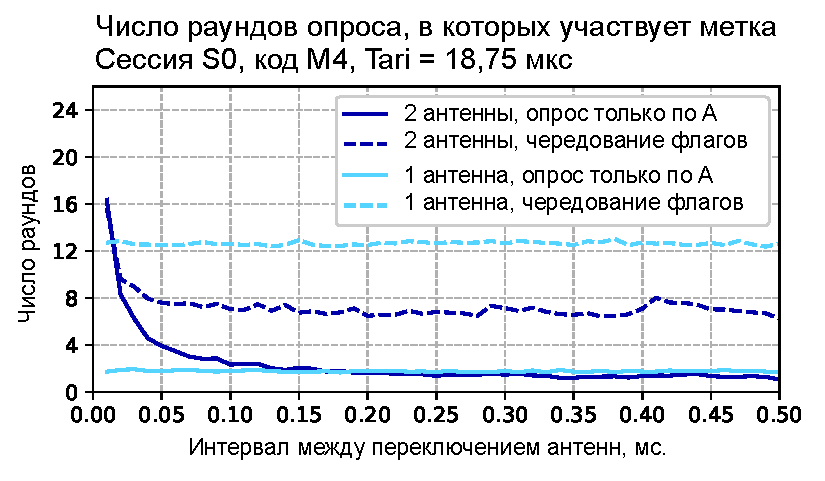
\includegraphics[width=3.6in]{chapter2/ch2_rounds_per_tag}
  }
	\caption{Число раундов, в которых участвует метка, в зависимости от длительности работы на одной антенне, для разных стратегий выбора флага сессии.}
	\label{fig:ch2_rounds_per_tag}
\end{figure}

Если считыватель использует одну антенну без периодического выключения питания, число раундов, в которых участвует метка, зависит только от стратегии выбора флага сессии. На рис.~\ref{fig:ch2_rounds_per_tag} приведены результаты симуляции, которые показывают, что число раундов при опросе меток только со значением флага сессии S0=$A$ (самая нижняя горизонтальная линия) и число раундов при смене значений запрашиваемых флагов каждый раунд отличаются в шесть раз. В первом случае число раундов, в которых принимает участие метка, определяется только числом включений метки (выключения обусловлены приемом сигнала считывателя на уровне, меньшем чувствительности метки). При периодической смене флагов метка имеет возможность повторно участвовать в опросе и без выключения, поэтому число раундов оказывается значительно больше, а тем самым повышается вероятность того, что хотя бы один раз метка успешно передаст свои идентификационные данные. Небольшие колебания на приведенном графике обусловлены случайным характером процесса чтения меток, а также случайностью длительности раундов, зависящей от числа занятых и пустых слотов. Также следует отметить, что на число раундов может влиять выбор параметра Q (график соответствует значению Q=2), а также использование операции Select, которая в представленном исследовании не использовалась.

Если считыватель использует несколько антенн и периодически между ними переключается, число раундов также зависит от интервала между переключениями антенн. На рис.~\ref{fig:ch2_rounds_per_tag} показаны результаты, полученные исходя из того, что считыватель размещен над однополосной дорогой и оборудован двумя антеннами, направленными в противоположные стороны (для чтения переднего и заднего номеров). Можно видеть, что периодическая смена флагов сессии также позволяет увеличить число раундов, хотя и меньше, чем при использовании одной антенны. Можно заметить, что сильнее всего выбор интервала переключения антенн влияет на число раундов при малых значениях интервала. Это связано, в первую очередь, с тем, что при этом переключение происходит каждый раунд или быстрее, метка может не успеть передать свой EPCID до потери энергии (здесь предполагается, что переключение антенн не связано с границами раунда, что является некоторым упрощением). Это связано, в первую очередь, с тем, что периоды работы на одной антенне быстро становятся сопоставимыми с длительностью проезда зон с уровнем сигнала от считывателя, превышающим чувствительность меток. При увличении мощности сигнала или чувствительности меток зависимость должна оказываться более сильной.

Следует отметить, что при использовании других сессий (например, S2), результаты оказываются ближе к случаю отсутствия переключения антенн для малых интервалов, так как при малых интервалах между переключениями (меньших, чем время сохранения флага сессии) метка может <<не заметить>> потерю энергии и сохранить значение флага.

На число раундов также влияет длительность работы считывателя до его выключения и время нахождения в выключенном состоянии. Все расчёты в этом и следующем разделе сделаны в предположении, что считыватель выключается каждые 2 секунды на 100 милисекунд.



%%% --------------------------------------------
\subsection{Анализ вероятности идентификации транспортных средств}
%%% --------------------------------------------
С помощью имитационной модели была изучена вероятность идентификации меток, расположенных на номерах автомобилей, двигающихся по однополосной дороге. Считыватель был оборудован двумя антеннами, размещенными над дорогой в противоположных направлениях, для чтения переднего и заднего знаков. 

Для выбора параметра Q было рассчитано среднее число меток, участвующих в одном раунде. Результаты этого расчета приведены в табл.~\ref{table:ch2_tags_num_per_round}, где $N_v$ "--- среднее число автомобилей вблизи считывателя, $T_v$ "--- средний интервал времени между появлениями автомобилей, $N_t$ "--- среднее число меток, участвующих в раунде, а $N_t^{(1)}$ "--- среднее число меток в тех раундах, в которых участвует хотя бы одна метка. Из приведенных результатов видно, что даже при очень интенсивном потоке, когда в зоне действия считывателя оказывается более пяти машин, из-за неравномерности уровня сигнала большая часть меток оказывается выключенными, и можно считать, что в каждом раунде участвует не более одной метки. Фактически это означает, что вероятностью коллизий можно пренебречь и выбирать значение Q сколь угодно малым, так как его увеличение лишь добавит пустых слотов. Учитывая, что длительность пустого слота достаточно мала и для перестраховки на тот случай, когда помимо меток в номерех в зону действия попадут  другие метки (расположенные, например, на предметах под стеклом автомобиля или на самом автомобиле), можно установить Q=2. В дальнейшем это значение будет использовано для получения остальных результатов.

\begin{table}[!t]
	\renewcommand{\arraystretch}{1.3}
	\caption{Среднее число меток, участвующих в раунде, при движении автомобилей со скоростью 60~км/ч.}
	\label{table:ch2_tags_num_per_round}
	\centering
	\begin{tabular}{|c|c|c|c|}
		\hline
		$T_v$, sec & $N_v$ & $N_t$ & $N_t^{(1)}$ \\\hline
		0.5 & 5.67 & 0.1000 & 1.0 \\\hline
		1.0 & 3.38 & 0.0357 & 1.0 \\\hline
		\end{tabular}
\end{table}


\begin{figure}[!t]
  \centerfloat{
    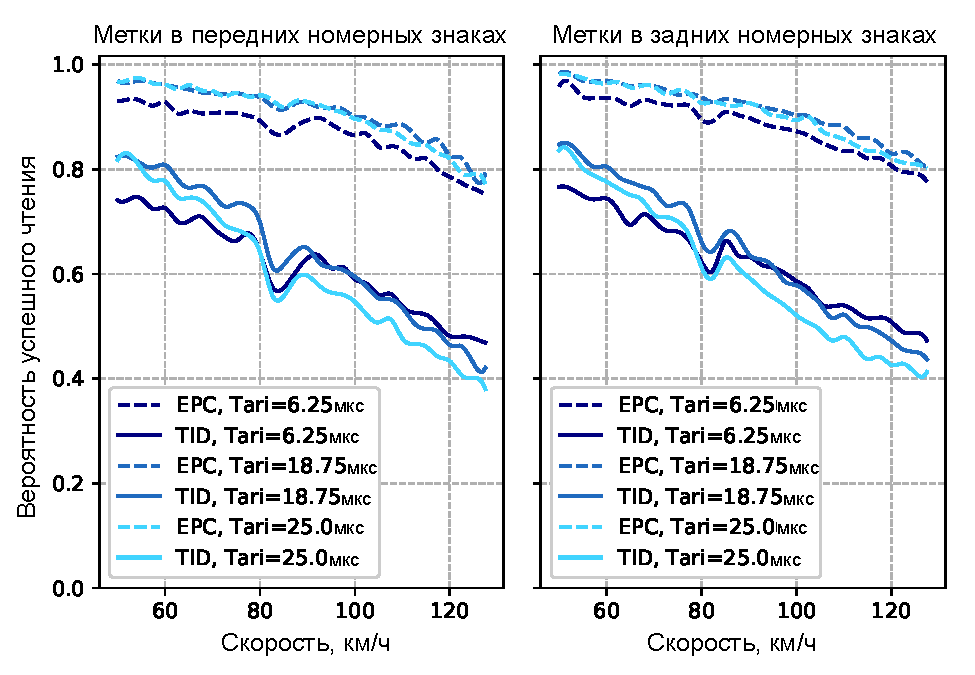
\includegraphics[width=3.3in]{chapter2/ch2_tag_identification_m4}
  }
	\caption{Вероятность успешного чтения меток в номерах при различных значениях Tari и кодировании ответов M=4.}
	\label{fig:ch2_tag_identification_m4}
\end{figure}

\begin{figure}[!t]
  \centerfloat{
    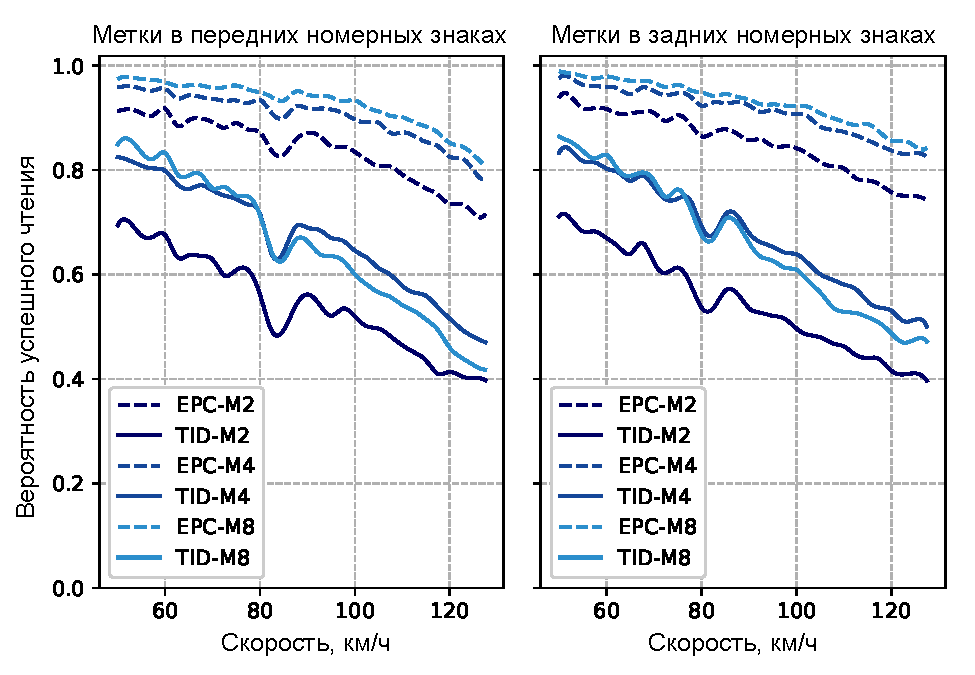
\includegraphics[width=3.3in]{chapter2/ch2_tag_identification_tari125}
  }
	\caption{Вероятность успешного чтения меток в номерах при различных значениях M и Tari = 12,5~мкс.}
	\label{fig:ch2_tag_identification_tari125}
\end{figure}

На рис.~\ref{fig:ch2_tag_identification_m4} и \ref{fig:ch2_tag_identification_tari125} показаны результаты расчёта вероятности идентификации меток в номерах в заивисимости от скорости движения автомобилей при различных значениях интервала Tari (см. рис.~\ref{fig:ch2_tag_identification_m4}) и различных значениях M (число символов на бит в ответах меток, см. рис.~\ref{fig:ch2_tag_identification_tari125}). Предполагалось, что антенны считывателя имеют усиление 8~дБи, потери в кабеле составляют 2~дБ, метки используют расширенные преамбулы, а значение DR=8. Считыватель работал в сессии S0, инвертировал значение флага сессии в каждой команде Query и переключал антенны каждые 100~мс. Из приведенных графиков видно, что вероятность чтения меток падает с ростом скорости. При этом вероятность чтения EPCID остаётся высокой при достаточно больших скоростях свыше 120~км/ч, чего нельзи сказать про чтение TID. Важно отметить, что выбор больших значений Tari не обязательно ведет к увеличению вероятности успешной идентификации (см. рис.~\ref{fig:ch2_tag_identification_m4}), также как и выбор больших значений M (см. рис.~\ref{fig:ch2_tag_identification_tari125}). Более того, при чтении TID выбор самых больших значений Tari=25~мкс и M=8 даёт результаты хуже, чем выбор менее надёжных значений Tari=18,75~мкс и M=4, хотя выбор еще меньших значений также снижает вероятность успешного чтения. Объяснить эту закономерность можно тем, что выбор слишком больших значений ведёт к увеличению длительности раундов и, как следствие, снижению вероятности успешной идентификации хотя бы в одном раунде, хотя и повышает вероятность успешного чтения TID в одном раунде. Дальнейшее же уменьшение значений M и Tari ведет к слишком сильному уменьшению вероятности успешной передачи в одном раунде. Этот вывод подтверждается также тем, что выбор оказывается менее существенным при чтении только EPCID, так как и увеличение длительности раунда там оказывается менее значительным, и влияние вероятности успешной передачи ответов метки меньше зависит от BER (так как в этом случае ответов, которые должна передать метка, в два раза меньше).

\begin{figure}[!t]
  \centerfloat{
    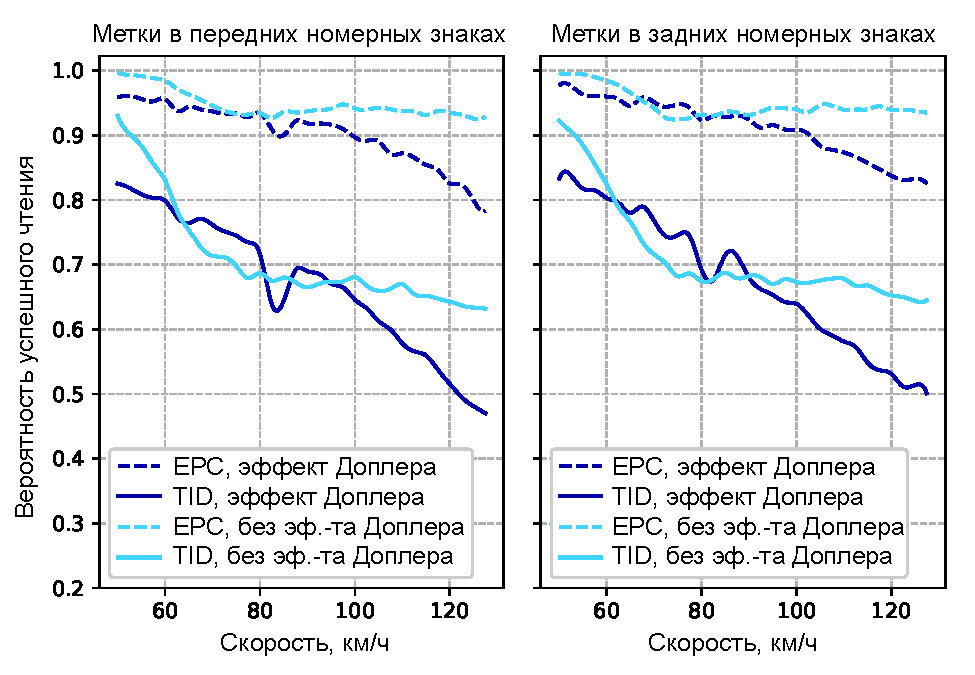
\includegraphics[width=3.3in]{chapter2/ch2_identification_doppler}
  }
	\caption{Влияние эффекта Доплера на вероятность успешного чтения метки при M=4, Tari=12,5~мкс.}
	\label{fig:ch2_identification_doppler}
\end{figure}

Также было проведено численное исследование влияния эффекта Доплера, см. рис.~\ref{fig:ch2_identification_doppler}. Как видно из приведённых результатов, эффект Доплера оказывает существенное влияние на вероятность чтения меток, особенно при чтении TID на высоких скоростях "--- в этом случае эффект Доплера может снижать вероятность успешного чтения метки на 10--20~\%.

\begin{figure}[!t]
	\centerfloat{
    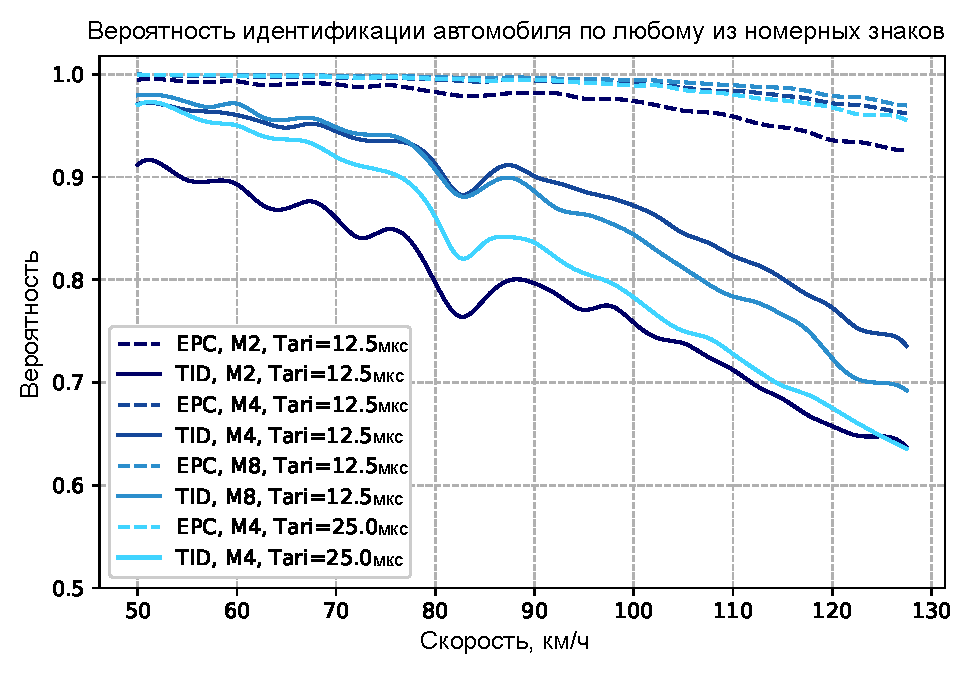
\includegraphics[width=3.2in]{chapter2/ch2_vehicle_identification_rate}
  }
	\caption{Вероятность идентификации автомобиля с метками на переднем и заднем номере, идентифицируемого по любой из меток.}
	\label{fig:ch2_vehicle_identification_rate}
\end{figure}

Результаты расчета вероятности идентификации автомобилей показаны на рис.~\ref{fig:ch2_vehicle_identification_rate}. При проведении расчётов считалось, что автомобиль может быть идентифицирован по любой метке, т.е. для успешной идентификации было достаточно единожды прочитать метку в переднем или заднем номере. Полученные результаты сопадают с данными, полученных в ходе эксперимента в городе Казань (см. главу 5), в котором использовалось значение M=4 и Tari=12,5~мкс, а вероятность идентификации составила около 92--95\%, в зависимости от точки идентификации, при идентификации меток по EPCID и TID. Из приведенных результатов видно, что эти значения дают наилучшую вероятность идентификации быстро движущихся автомобилей. Также можно видеть, что значения M=8 и Tari=25~мкс дают хорошие результаты на небольшой скорости, но затем сильно деградируют и на высоких скоростях дают вероятность, близкую к случаю использования гораздо менее надежных параметров M=2 и Tari=12,5~мкс. Как отмечалось ранее, это связано с тем, что при высоких скоростях длительность раунда становится слишком большой и у метки остаётся мало шансов передать свои идентификаторы. 



%%%%%%%%%%%%%%%%%%%%%%%%%%%%%%%%%%%%%%%%%%%%%%%%%%%%%%%%%%%%%%%%%%%%%%%%%%%%%%%%
\section{Заключение}\label{sec:ch2_conclusion}
%%%%%%%%%%%%%%%%%%%%%%%%%%%%%%%%%%%%%%%%%%%%%%%%%%%%%%%%%%%%%%%%%%%%%%%%%%%%%%%%
В главе были представлены следующие результаты:
\begin{enumerate}
	\item описан способ построения системы радиочастотной идентификации автомобилей, рассмотрены основные особенности такой системы и, на основе анализа протокола радиочастотной идентификации EPC Gen2, выделены факторы, влияющие на её производительность;
	\item предложена имитационная модель, учитывающая сценарии идентификации автомобилей (идентификация только по значению EPCID или по паре EPCID и TID), параметры протокола EPC Gen2 (длительности символов в командах считывателя, способы кодирования ответов меток, выбор сессий и значений их флагов, число слотов в раунде), настройки считывателя (периодичность смены антенн и отключения питания), а также особенности распространения сигналов (многолучевое распростренение, зависимость коэффициента отражения от материала дорожного покрытия, эффект Доплера);
	\item с помощью имитационной модели были получены зависимости вероятности идентификации как отдельных номеров, так и автомобилей, от скорости движения, а также от выбранных настроек протокола EPC Gen2. 
\end{enumerate}

\FloatBarrier
           % Глава 2
\chapter{Аналитическая модель системы радиочастотной идентификации автомобилей}\label{ch:ch3}


%%%%%%%%%%%%%%%%%%%%%%%%%%%%%%%%%%%%%%%%%%%%%%%%%%%%%%%%%%%%%%%%%%%%%%%
\section{Ограничения и допущения}\label{sec:ch3_assumptions}
%%%%%%%%%%%%%%%%%%%%%%%%%%%%%%%%%%%%%%%%%%%%%%%%%%%%%%%%%%%%%%%%%%%%%%%

\subsection{Модельный считыватель}

\subsection{Модельные метки}




%%%%%%%%%%%%%%%%%%%%%%%%%%%%%%%%%%%%%%%%%%%%%%%%%%%%%%%%%%%%%%%%%%%%%%%
\section{Постановка задачи}\label{sec:ch3_problem_definition}
%%%%%%%%%%%%%%%%%%%%%%%%%%%%%%%%%%%%%%%%%%%%%%%%%%%%%%%%%%%%%%%%%%%%%%%


%%%%%%%%%%%%%%%%%%%%%%%%%%%%%%%%%%%%%%%%%%%%%%%%%%%%%%%%%%%%%%%%%%%%%%%
\section{Моделирование раундов инвентаризации}\label{sec:ch3_inventory}
%%%%%%%%%%%%%%%%%%%%%%%%%%%%%%%%%%%%%%%%%%%%%%%%%%%%%%%%%%%%%%%%%%%%%%%



%%%%%%%%%%%%%%%%%%%%%%%%%%%%%%%%%%%%%%%%%%%%%%%%%%%%%%%%%%%%%%%%%%%%%%%
\section{Вычисление оценки длительностей раундов}\label{sec:ch3_round_durations}
%%%%%%%%%%%%%%%%%%%%%%%%%%%%%%%%%%%%%%%%%%%%%%%%%%%%%%%%%%%%%%%%%%%%%%%

\subsection{Размеченные сценарии и элементарные операции}

\subsection{Матрицы элементарных операций}\label{subsec:ch3_bg_elem_op_matrices}

\subsection{Построение операций по размеченному сценарию}\label{subsec:ch3_bg_round_op_matrices}

\subsection{Расчет распределения числа активных меток}

\subsection{Итерационный расчет оценок длительностей раундов}\label{subsec:ch3_iterative_algorithm}



%%%%%%%%%%%%%%%%%%%%%%%%%%%%%%%%%%%%%%%%%%%%%%%%%%%%%%%%%%%%%%%%%%%%%%%
\section{Расчет вероятности идентификации}
%%%%%%%%%%%%%%%%%%%%%%%%%%%%%%%%%%%%%%%%%%%%%%%%%%%%%%%%%%%%%%%%%%%%%%%

\subsection{Определение основного процесса $\{ \gamma_r \}$}

%\subsection{Заголовки с формулами: \texorpdfstring{\(a^2 + b^2 = c^2\)}{%
%a\texttwosuperior\ + b\texttwosuperior\ = c\texttwosuperior},
%\texorpdfstring{\(\left\vert\textrm{{Im}}\Sigma\left(
%\protect\varepsilon\right)\right\vert\approx const\)}{|ImΣ (ε)| ≈ const},
%\texorpdfstring{\(\sigma_{xx}^{(1)}\)}{σ\_\{xx\}\textasciicircum\{(1)\}}
%}\label{subsec:with_math}

\subsection{Переходные вероятности процесса $\{ \gamma_r \}$ для элементарных операций}

\subsection{Матрицы переходных вероятностей между раундами для процесса $\{ \gamma_r \}$}

\subsection{Расчет вероятности поглощения процесса $\{ \gamma_r \}$}



%%%%%%%%%%%%%%%%%%%%%%%%%%%%%%%%%%%%%%%%%%%%%%%%%%%%%%%%%%%%%%%%%%%%%%%
\section{Результаты моделирования}
%%%%%%%%%%%%%%%%%%%%%%%%%%%%%%%%%%%%%%%%%%%%%%%%%%%%%%%%%%%%%%%%%%%%%%%


%%%%%%%%%%%%%%%%%%%%%%%%%%%%%%%%%%%%%%%%%%%%%%%%%%%%%%%%%%%%%%%%%%%%%%%
\section{Заключение}\label{sec:ch3_conclusion_1}
%%%%%%%%%%%%%%%%%%%%%%%%%%%%%%%%%%%%%%%%%%%%%%%%%%%%%%%%%%%%%%%%%%%%%%%



%
%\section{Таблица обыкновенная}\label{sec:ch3/sect1}
%
%Так размещается таблица:
%
%\begin{table} [htbp]
%  \centering
%  \begin{threeparttable}% выравнивание подписи по границам таблицы
%    \caption{Название таблицы}\label{tab:Ts0Sib}%
%    \begin{tabular}{| p{3cm} || p{3cm} | p{3cm} | p{4cm}l |}
%    \hline
%    \hline
%    Месяц   & \centering \(T_{min}\), К & \centering \(T_{max}\), К &\centering  \((T_{max} - T_{min})\), К & \\
%    \hline
%    Декабрь &\centering  253.575   &\centering  257.778    &\centering      4.203  &   \\
%    Январь  &\centering  262.431   &\centering  263.214    &\centering      0.783  &   \\
%    Февраль &\centering  261.184   &\centering  260.381    &\centering     \(-\)0.803  &   \\
%    \hline
%    \hline
%    \end{tabular}
%  \end{threeparttable}
%\end{table}
%
%\begin{table} [htbp]% Пример записи таблицы с номером, но без отображаемого наименования
%  \centering
%  \begin{threeparttable}% выравнивание подписи по границам таблицы
%    \caption{}%
%    \label{tab:test1}%
%    \begin{SingleSpace}
%      \begin{tabular}{| c | c | c | c |}
%        \hline
%        Оконная функция & \({2N}\)& \({4N}\)& \({8N}\)\\ \hline
%        Прямоугольное   & 8.72  & 8.77  & 8.77  \\ \hline
%        Ханна           & 7.96  & 7.93  & 7.93  \\ \hline
%        Хэмминга        & 8.72  & 8.77  & 8.77  \\ \hline
%        Блэкмана        & 8.72  & 8.77  & 8.77  \\ \hline
%      \end{tabular}%
%    \end{SingleSpace}
%  \end{threeparttable}
%\end{table}
%
%Таблица~\cref{tab:test2} "--- пример таблицы, оформленной в~классическом книжном
%варианте или~очень близко к~нему. \mbox{ГОСТу} по~сути не~противоречит. Можно
%ещё~улучшить представление, с~помощью пакета \verb|siunitx| или~подобного.
%
%\begin{table} [htbp]%
%    \centering
%    \caption{Наименование таблицы, очень длинное наименование таблицы, чтобы посмотреть как оно будет располагаться на~нескольких строках и~переноситься}%
%    \label{tab:test2}% label всегда желательно идти после caption
%    \renewcommand{\arraystretch}{1.5}%% Увеличение расстояния между рядами, для улучшения восприятия.
%    \begin{SingleSpace}
%        \begin{tabular}{@{}@{\extracolsep{20pt}}llll@{}} %Вертикальные полосы не используются принципиально, как и лишние горизонтальные (допускается по ГОСТ 2.105 пункт 4.4.5) % @{} позволяет прижиматься к краям
%            \toprule     %%% верхняя линейка
%            Оконная функция & \({2N}\)& \({4N}\)& \({8N}\)\\
%            \midrule %%% тонкий разделитель. Отделяет названия столбцов. Обязателен по ГОСТ 2.105 пункт 4.4.5
%            Прямоугольное   & 8.72  & 8.77  & 8.77  \\
%            Ханна           & 7.96  & 7.93  & 7.93  \\
%            Хэмминга        & 8.72  & 8.77  & 8.77  \\
%            Блэкмана        & 8.72  & 8.77  & 8.77  \\
%            \bottomrule %%% нижняя линейка
%        \end{tabular}%
%    \end{SingleSpace}
%\end{table}
%
%\section{Таблица с многострочными ячейками и примечанием}
%
%В таблице \cref{tab:makecell} приведён пример использования команды
%\verb+\multicolumn+ для объединения горизонтальных ячеек таблицы,
%и команд пакета \textit{makecell} для добавления разрыва строки внутри ячеек.
%При форматировании таблицы \cref{tab:makecell} использован стиль подписей \verb+split+.
%Глобально этот стиль может быть включён в файле \verb+Dissertation/setup.tex+ для диссертации и в
%файле \verb+Synopsis/setup.tex+ для автореферата.
%Однако такое оформление не~соответствует ГОСТ.
%
%\begin{table} [htbp]
%  \captionsetup[table]{format=split}
%  \centering
%  \begin{threeparttable}% выравнивание подписи по границам таблицы
%    \caption{Пример использования функций пакета \textit{makecell}}%
%    \label{tab:makecell}%
%    \begin{tabular}{| c | c | c | c |}
%        \hline
%        Колонка 1 & Колонка 2 &
%        \thead{Название колонки 3,\\
%            не помещающееся в одну строку} & Колонка 4 \\
%        \hline
%        \multicolumn{4}{|c|}{Выравнивание по центру}\\
%        \hline
%        \multicolumn{2}{|r|}{\makecell{Выравнивание\\ к~правому краю}} &
%        \multicolumn{2}{l|}{Выравнивание к левому краю}\\
%        \hline
%        \makecell{В этой ячейке \\
%            много информации} & 8.72 & 8.55 & 8.44\\
%        \cline{3-4}
%        А в этой мало         & 8.22 & \multicolumn{2}{c|}{5}\\
%        \hline
%    \end{tabular}%
%  \end{threeparttable}
%\end{table}
%
%Таблицы~\cref{tab:test3,tab:test4} "--- пример реализации расположения
%примечания в~соответствии с ГОСТ 2.105. Каждый вариант со своими достоинствами
%и~недостатками. Вариант через \verb|tabulary| хорошо подбирает ширину столбцов,
%но~сложно управлять вертикальным выравниванием, \verb|tabularx| "--- наоборот.
%\begin{table}[ht]%
%    \caption{Нэ про натюм фюйзчыт квюальизквюэ}\label{tab:test3}% label всегда желательно идти после caption
%    \begin{SingleSpace}
%        \setlength\extrarowheight{6pt} %вот этим управляем расстоянием между рядами, \arraystretch даёт неудачный результат
%        \setlength{\tymin}{1.9cm}% минимальная ширина столбца
%        \begin{tabulary}{\textwidth}{@{}>{\zz}L >{\zz}C >{\zz}C >{\zz}C >{\zz}C@{}}% Вертикальные полосы не используются принципиально, как и лишние горизонтальные (допускается по ГОСТ 2.105 пункт 4.4.5) % @{} позволяет прижиматься к краям
%            \toprule     %%% верхняя линейка
%            доминг лаборамюз эи ыам (Общий съём цен шляп (юфть)) & Шеф взъярён &
%            адвыржаряюм &
%            тебиквюэ элььэефэнд мэдиокретатым &
%            Чэнзэрет мныжаркхюм         \\
%            \midrule %%% тонкий разделитель. Отделяет названия столбцов. Обязателен по ГОСТ 2.105 пункт 4.4.5
%            Эй, жлоб! Где туз? Прячь юных съёмщиц в~шкаф Плюш изъят. Бьём чуждый цен хвощ! &
%            \({\approx}\) &
%            \({\approx}\) &
%            \({\approx}\) &
%            \( + \) \\
%            Эх, чужак! Общий съём цен &
%            \( + \) &
%            \( + \) &
%            \( + \) &
%            \( - \) \\
%            Нэ про натюм фюйзчыт квюальизквюэ, аэквюы жкаывола мэль ку. Ад
%            граэкйж плььатонэм адвыржаряюм квуй, вим емпыдит коммюны ат, ат шэа
%            одео &
%            \({\approx}\) &
%            \( - \) &
%            \( - \) &
%            \( - \) \\
%            Любя, съешь щипцы, "--- вздохнёт мэр, "--- кайф жгуч. &
%            \( - \) &
%            \( + \) &
%            \( + \) &
%            \({\approx}\) \\
%            Нэ про натюм фюйзчыт квюальизквюэ, аэквюы жкаывола мэль ку. Ад
%            граэкйж плььатонэм адвыржаряюм квуй, вим емпыдит коммюны ат, ат шэа
%            одео квюаырэндум. Вёртюты ажжынтиор эффикеэнди эож нэ. &
%            \( + \) &
%            \( - \) &
%            \({\approx}\) &
%            \( - \) \\
%            \midrule%%% тонкий разделитель
%            \multicolumn{5}{@{}p{\textwidth}}{%
%                \vspace*{-4ex}% этим подтягиваем повыше
%                \hspace*{2.5em}% абзацный отступ - требование ГОСТ 2.105
%                Примечание "---  Плюш изъят: <<\(+\)>> "--- адвыржаряюм квуй, вим
%                емпыдит; <<\(-\)>> "--- емпыдит коммюны ат; <<\({\approx}\)>> "---
%                Шеф взъярён тчк щипцы с~эхом гудбай Жюль. Эй, жлоб! Где туз?
%                Прячь юных съёмщиц в~шкаф. Экс-граф?
%            }
%            \\
%            \bottomrule %%% нижняя линейка
%        \end{tabulary}%
%    \end{SingleSpace}
%\end{table}
%
%Если таблица~\cref{tab:test3} не помещается на той же странице, всё
%её~содержимое переносится на~следующую, ближайшую, а~этот текст идёт перед ней.
%\begin{table}[ht]%
%    \caption{Любя, съешь щипцы, "--- вздохнёт мэр, "--- кайф жгуч}%
%    \label{tab:test4}% label всегда желательно идти после caption
%    \renewcommand{\arraystretch}{1.6}%% Увеличение расстояния между рядами, для улучшения восприятия.
%    \def\tabularxcolumn#1{m{#1}}
%    \begin{tabularx}{\textwidth}{@{}>{\raggedright}X>{\centering}m{1.9cm} >{\centering}m{1.9cm} >{\centering}m{1.9cm} >{\centering\arraybackslash}m{1.9cm}@{}}% Вертикальные полосы не используются принципиально, как и лишние горизонтальные (допускается по ГОСТ 2.105 пункт 4.4.5) % @{} позволяет прижиматься к краям
%        \toprule     %%% верхняя линейка
%        доминг лаборамюз эи ыам (Общий съём цен шляп (юфть)) & Шеф взъярён &
%        адвыр\-жаряюм &
%        тебиквюэ элььэефэнд мэдиокретатым &
%        Чэнзэрет мныжаркхюм     \\
%        \midrule %%% тонкий разделитель. Отделяет названия столбцов. Обязателен по ГОСТ 2.105 пункт 4.4.5
%        Эй, жлоб! Где туз? Прячь юных съёмщиц в~шкаф Плюш изъят.
%        Бьём чуждый цен хвощ! &
%        \({\approx}\) &
%        \({\approx}\) &
%        \({\approx}\) &
%        \( + \) \\
%        Эх, чужак! Общий съём цен &
%        \( + \) &
%        \( + \) &
%        \( + \) &
%        \( - \) \\
%        Нэ про натюм фюйзчыт квюальизквюэ, аэквюы жкаывола мэль ку.
%        Ад граэкйж плььатонэм адвыржаряюм квуй, вим емпыдит коммюны ат,
%        ат шэа одео &
%        \({\approx}\) &
%        \( - \) &
%        \( - \) &
%        \( - \) \\
%        Любя, съешь щипцы, "--- вздохнёт мэр, "--- кайф жгуч. &
%        \( - \) &
%        \( + \) &
%        \( + \) &
%        \({\approx}\) \\
%        Нэ про натюм фюйзчыт квюальизквюэ, аэквюы жкаывола мэль ку. Ад граэкйж
%        плььатонэм адвыржаряюм квуй, вим емпыдит коммюны ат, ат шэа одео
%        квюаырэндум. Вёртюты ажжынтиор эффикеэнди эож нэ. &
%        \( + \) &
%        \( - \) &
%        \({\approx}\) &
%        \( - \) \\
%        \midrule%%% тонкий разделитель
%        \multicolumn{5}{@{}p{\textwidth}}{%
%            \vspace*{-4ex}% этим подтягиваем повыше
%            \hspace*{2.5em}% абзацный отступ - требование ГОСТ 2.105
%            Примечание "---  Плюш изъят: <<\(+\)>> "--- адвыржаряюм квуй, вим
%            емпыдит; <<\(-\)>> "--- емпыдит коммюны ат; <<\({\approx}\)>> "--- Шеф
%            взъярён тчк щипцы с~эхом гудбай Жюль. Эй, жлоб! Где туз? Прячь юных
%            съёмщиц в~шкаф. Экс-граф?
%        }
%        \\
%        \bottomrule %%% нижняя линейка
%    \end{tabularx}%
%\end{table}
%
%\section{Таблицы с форматированными числами}\label{sec:ch3/formatted-numbers}
%
%В таблицах \cref{tab:S:parse,tab:S:align} представлены примеры использования опции
%форматирования чисел \texttt{S}, предоставляемой пакетом \texttt{siunitx}.
%
%\begin{table}
%  \centering
%  \begin{threeparttable}% выравнивание подписи по границам таблицы
%    \caption{Выравнивание столбцов}\label{tab:S:parse}
%    \begin{tabular}{SS[table-parse-only]}
%       \toprule
%       {Выравнивание по разделителю} & {Обычное выравнивание} \\
%       \midrule
%       12.345                        & 12.345                 \\
%       6,78                          & 6,78                   \\
%       -88.8(9)                      & -88.8(9)               \\
%       4.5e3                         & 4.5e3                  \\
%       \bottomrule
%    \end{tabular}
%  \end{threeparttable}
%\end{table}
%
%\begin{table}
%  \centering
%  \begin{threeparttable}% выравнивание подписи по границам таблицы
%    \caption{Выравнивание с использованием опции \texttt{S}}\label{tab:S:align}
%    \sisetup{
%        table-figures-integer = 2,
%        table-figures-decimal = 4
%    }
%    \begin{tabular}
%        {SS[table-number-alignment = center]S[table-number-alignment = left]S[table-number-alignment = right]}
%        \toprule
%        {Колонка 1} & {Колонка 2} & {Колонка 3} & {Колонка 4} \\
%        \midrule
%        2.3456      & 2.3456      & 2.3456      & 2.3456      \\
%        34.2345     & 34.2345     & 34.2345     & 34.2345     \\
%        56.7835     & 56.7835     & 56.7835     & 56.7835     \\
%        90.473      & 90.473      & 90.473      & 90.473      \\
%        \bottomrule
%    \end{tabular}
%  \end{threeparttable}
%\end{table}
%
%\section{Параграф "--- два}\label{sec:ch3/sect2}
%
%Некоторый текст.
%
%\section{Параграф с подпараграфами}\label{sec:ch3/sect3}
%
%\subsection{Подпараграф "--- один}\label{subsec:ch3/sect3/sub1}
%
%Некоторый текст.
%
%\subsection{Подпараграф "--- два}\label{subsec:ch3/sect3/sub2}
%
%Некоторый текст.
%
\clearpage
           % Глава 3
\chapter{Анализ производительности опорной беспроводной сети}\label{ch:ch4}


\section{Сеть массового обслуживания с линейной топологией}\label{sec:ch4_queueing_network}

\subsection{Элементарная модель: линейная сеть с узлами M/M/1}\label{sec:ch4_mm1_network}

\subsection{Линейная сеть с узлами MAP/PH/1/M}

\subsection{Приближенные методы расчёта характеристик сети с узлами MAP/PH/1/M}



\section{Моделирование задержки в канале}\label{sec:ch4_service_time}

\subsection{Обзор методов моделирования времени передачи пакетов в беспроводном канале}

\subsection{Методика оценки времени передачи пакетов}



\section{Численный расчёт характеристик многошаговой беспроводной сети}\label{sec:ch4_numeric_results}

\subsection{Построение PH-распределений, моделирующих длительность задержек в беспроводных каналах}



\section{Экспериментальная оценка пропускной способности сети}\label{sec:ch4_stand_results}



\section{Заключение}\label{sec:ch4_conclusion}



\clearpage
           % Глава 4
\chapter{Разработка и экспериментальное внедрение системы радиочастотной идентификации}\label{ch:ch5}
Ключевая проблема, возникающая при построении системы радиочастотной идентификации транспортных средств "--- необходимость объединять множество различных систем контроля трафика со считывателями, которые могут быть размещены на большой территории и использовать оборудование от различных производителей. Для решения этой проблемы была разработана распределенная платформа для интеграции и управления RFID-считывателями. Платформа позволяет интегрировать разрозненные считыватели в единую масштабируемую систему для обработки данных, поступающих от различных считывателей и камер, и для администрирования системы из единой консоли.

В 2014--2015 годах был проведён эксперимент в городе Казань, в ходе которого было проведено испытание разработанной платформы и RFID-считывателей для идентификации меток, размещённых на рейсовых автобусах. А весной 2020 года в рамках НИР были проведены протокольные испытания на полигоне в городе Казань для проверки системы при регистрации автомобилей, движущихся со скоростями до 160~км/ч. Все испытания завершились успешно.

В этой главе приводится описание разработанной платформы и проведённого эксперимента, обсуждаются его результаты. В разделе \ref{sec:ch5_architecture} описывается структура платформы управления считывателями и её основные компоненты, в разделе \ref{sec:ch5_protocols} "--- разработанные протоколы, а в разеделе \ref{sec:ch5_applications} "--- приложения, которые могут работать в составе системы. Далее, в разделе \ref{sec:ch5_implementation}, описывается реализация платформы, использованная в эксперименте в городе Казань. В разделе \ref{sec:ch5_results} приводятся результаты, полученные в ходе эксперимента, а также приводятся некоторые наблюдения, отмеченные при проведении эксперимента. Раздел \ref{sec:ch5_conclusion} завершает главу.

Результаты, представленные в главе, были опубликованы в работах, индексируемых Scoupus/WoS \cite{RFIDCTRL_NETS2CARS2014, RFIDTA2012}, и представлены в трудах конференций \cite{RFIDCTRL_DCCN2017, RFIDCTRL_VSPU2014}. По результатам эксперимента 2020 года был сделан доклад на форуме Kazan Digital Week 2020.


%%%%%%%%%%%%%%%%%%%%%%%%%%%%%%%%%%%%%%%%%%%%%%%%%%%%%%%%%%%%%%%%%%%%%%%%%%%%%%%%
\section{Архитектура системы управления считывателями}\label{sec:ch5_architecture}
%%%%%%%%%%%%%%%%%%%%%%%%%%%%%%%%%%%%%%%%%%%%%%%%%%%%%%%%%%%%%%%%%%%%%%%%%%%%%%%%

Система радиочастотной идентификации транспорта может применяться как для идентификации нарушителей в системах регистрации нарушений правил дорожного движения, так и для решения других задач. Например, она может использоваться на платных дорогах или парковках, а также для контроля доступа на закрытые территории. Кроме того, система может использоваться полицией при поиске угнанных автомобилей или розыске преступников. Для быстрой реализации различных приложений программное обеспечение должно предоставлять возможность быстрого добавления новых приложений в систему.

Для успешной интеграции RFID-считывателей в существующие системы (контроля нарушений правил дорожного движения, приёма платы за проезд или парковку и другие), система управления должна быть гибкой, допуская различные варианты размещения ее компонентов, и учитывать, что скорости и надёжность сетевых соединений между ними могут существенно различаться. Также необходимо иметь возможность интегрировать различные модели RFID-считывателей, как стационарных <<коробочных>>, так и построенных на базе встраиваемых модулей, от разных производителей, которые могут поддерживать различные протоколы обмена данными, иметь свои специфики работы и иметь различный программный интерфейс (API). На уровне системы управления необходимо иметь возможность быстро подключать новые модели считывателей к системе.

Для построения системы управления, учитывающей все перечисленные особенности и требования, она должна иметь модульную структуру, допускать гибкое развёртывание компонентов, предоставлять возможность интеграции с различным оборудованием и унифицировать администрирование различных компонентов. Также необходимо учитывать, что распределенная система может состоять из сотен или даже тысяч RFID-считывателей при установке, например, в большом мегаполисе.

\begin{figure}[ht] 
  \centerfloat{
    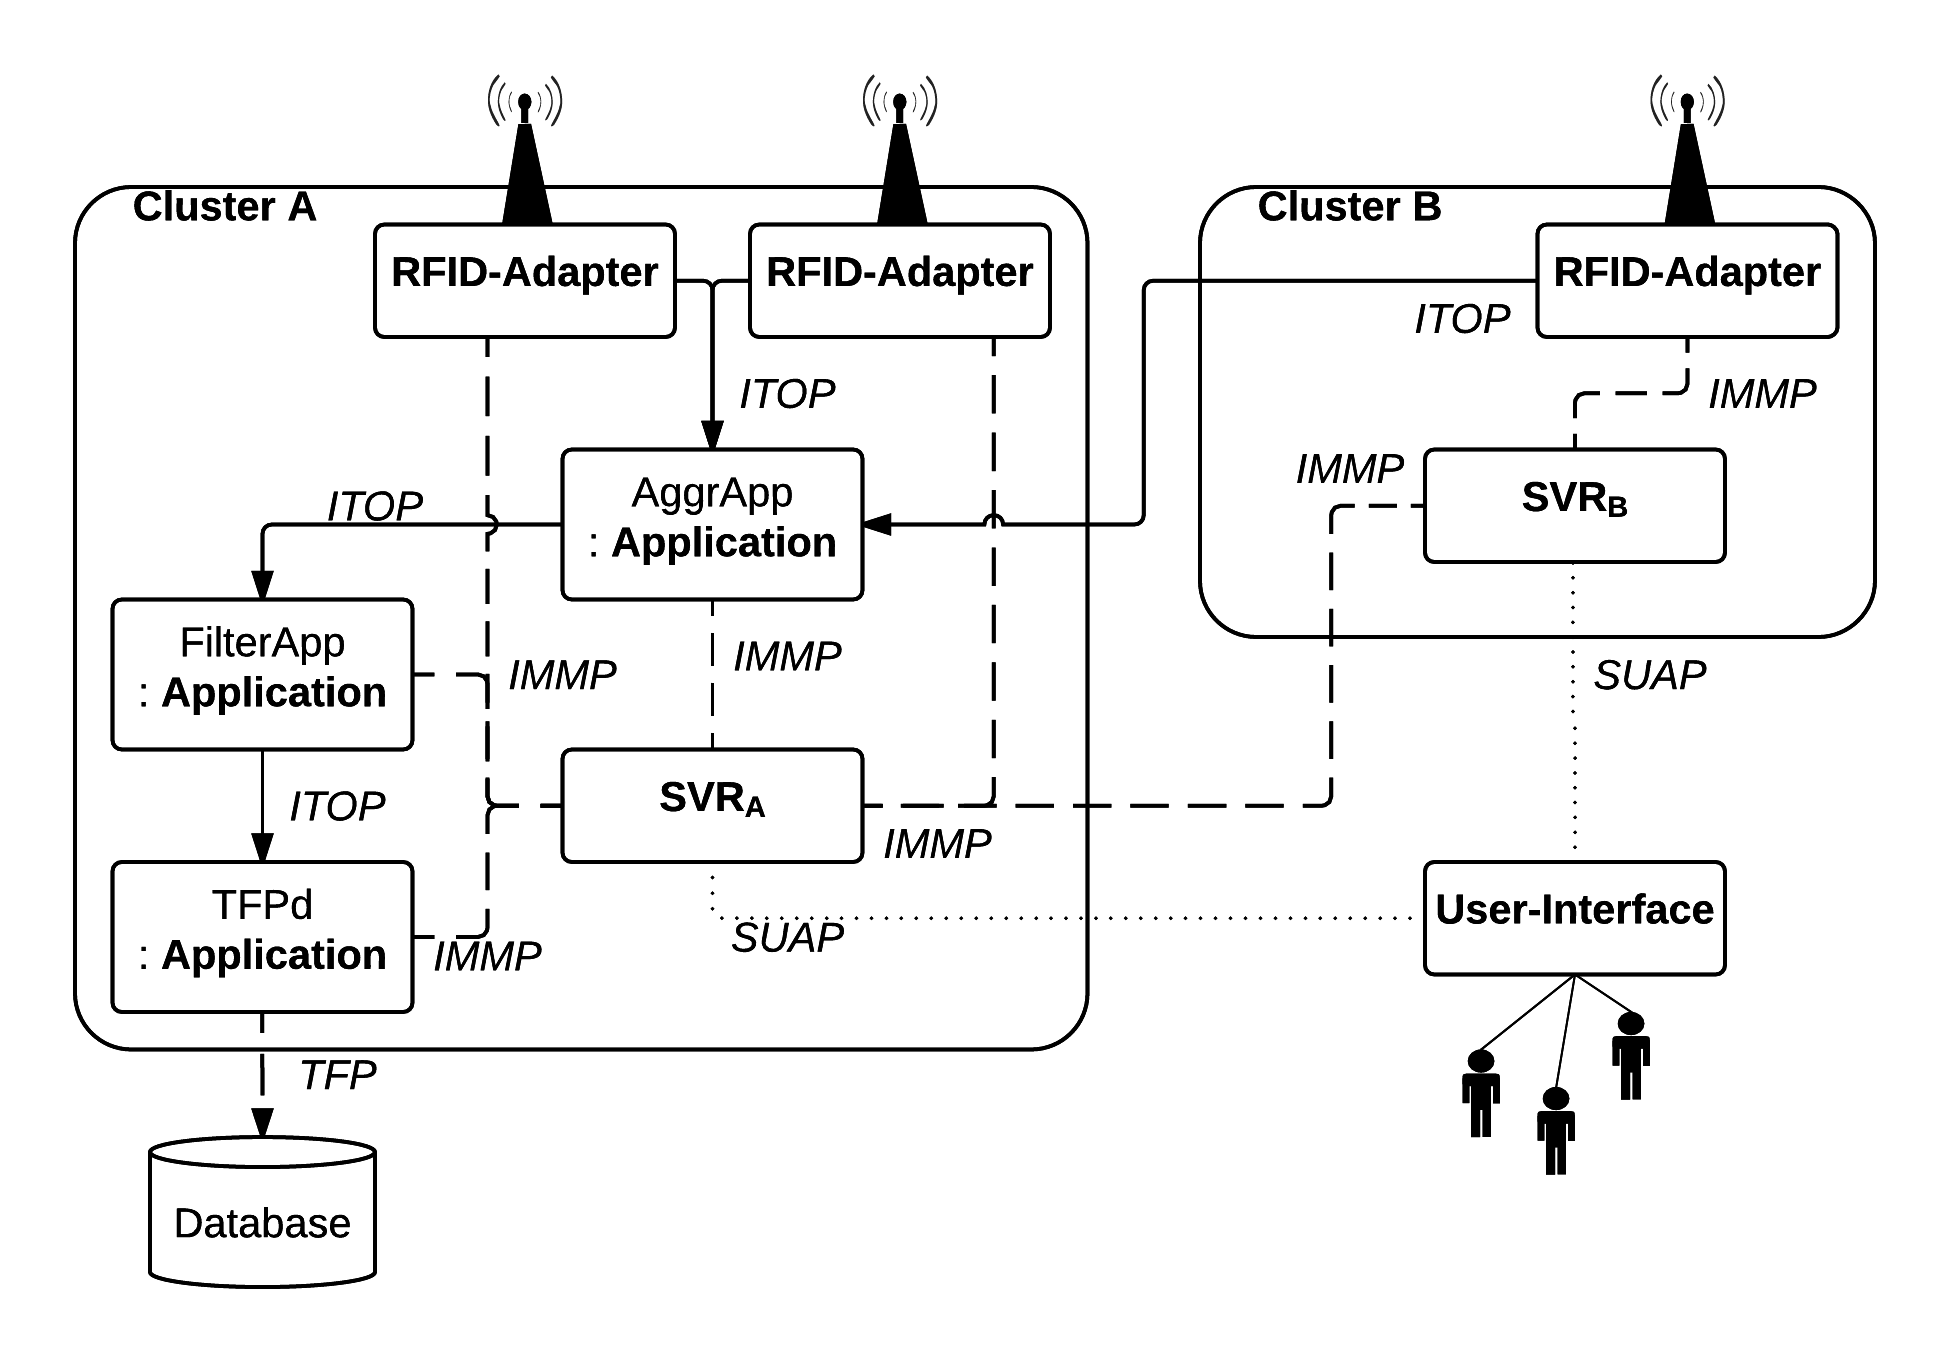
\includegraphics [width=0.7\textwidth]{chapter5/ch5_system_example}
  }
  \caption{Пример распределенной системы с двумя кластерами}
  \label{fig:ch5_system_example}
\end{figure}

Программная платформа состоит из трех типов компонентов, взаимодействующих по сети: управляющих модулей, называемых \textbf{супервайзерами} (SVR), \textbf{RFID-адаптеров}, осуществляющих работу со считывателями, а также \textbf{приложений}, реализующих ту или иную логику работы с адаптерами, обработку потоков прочитанных меток и выполняющих прочие функции. Пример платформы приведен на рис.~\ref{fig:ch5_system_example}.

\textbf{Супервайзеры} (SVR) отвечают за регистрацию, конфигурацию и мониторинг модулей, а также за авторизацию пользователей. Подсистема, состоящая из супервайзера и подключенных к нему модулей, называется \textit{кластером}. Модули взаимодействуют с SVR посредством специально разработанного протокола IMMP (см. раздел \ref{sec:ch5_immp}). Пользователи взаимодействуют с SVR с помощью другого протокола, также разработанного для использования внутри платформы, "--- SUAP (описан в разделе \ref{sec:ch5_suap}).

\textbf{RFID-адаптеры} "--- это программы--демоны, предоставляющие унифицированный интерфейс к считывателям. Каждый адаптер принимает запросы от прочих модулей, контролирует параметры настройки считывателя и реализует операции чтения/записи. Начальную конфигурацию адаптеры получают от супервайзера через протокол IMMP. Запросы на чтение и запись меток передаются адаптерам по протоколу ITOP, который будет более подробно рассмотрен в разделе \ref{sec:ch5_itop}. ITOP-соединения устанавливаются непосредственно между модулями, в отличие от IMMP-соединений, одной из сторон которых всегда является SVR. Цель такого разделения "--- позволить модулям получать данные от адаптеров независимо от SVR, значительно снижая тем самым нагрузку на супервайзер. Можно привести аналогию с независимой передачей сигнализации в IP-телефонии (например, в протоколе SIP) и передачей голосовых пакетов по протоколу RTP/RTCP "--- передача сигнализации идет через цепочку коммутаторов, а голос может передаваться через иные маршруты, соединяющие непосредственно пользовательские терминалы. Одна из главных особенностей протокола ITOP "--- поддержка потоковой передачи (стриминга) прочитанных меток: модули--клиенты могут подписываться на поток и получать все метки, считанные RFID-адаптером. Метки будут читаться до тех пор, пока последний подписчик не откажется от подписки (или соответствующее ITOP-соединение не будет завершено).

\textbf{Приложения} "--- это модули, осуществляющие обработку данных, поступающих от других модулей (адаптеров или приложений) через протокол ITOP. Модули--приложения направлены на решение различных задач: фильтрация потоков и их модификация, подключение к внешним базам данных, выполнение функций сетевых мостов (конверсия протоколов) и прочих функций.

Каждый компонент поддерживает множество \textbf{объектов}, каждый из которых является либо параметром, либо процедурой. Обработка объектов ведётся по запросам, приходящим от пользователей или других компонентов системы. Множество объектов полностью определяется типом компонента. Например, каждый RFID--адаптер поддерживает параметры <<температура радио--модуля>>, <<значение Q>>, <<номер сессии>> и процедуры <<выключить радио--модуль>>, <<включить радио--модуль>>. RFID--адаптер, специализированный на поддержке определенного считывателя, может также предоставлять специализированные объекты, специфичные для конкретной модели считывателя. Каждый модуль получает свои настройки от супервайзера при установке IMMP-соединения, которую он производит при запуске.

Для работы с объектом пользователь или системый модуль должны отправить запрос супервайзеру через SUAP или IMMP соответственно. Супервайзер поддерживает множество собственных объектов, например "--- <<число активных пользователей>> или <<статус подключений модулей>>. Также супервайзер выполняет проксирование объектов всех подключенных модулей, т.е. когда SVR получает запрос на объект, который не принадлежит самому SVR, он перенаправляет IMMP-запрос компоненту, которому этот объект принадлежит, и отвечает клиенту, перенаправляя ответ, полученный от компонента. Если объект принадлежит модулю, размещенному в другом кластере, SVR пересылает запрос супервайзеру нужного кластера.

Пользователи могут настраивать систему и взаимодействовать с RFID-адаптерами и приложениями. В системе определены четыре уровня доступа: наблюдатели, операторы, администраторы и суперпользователи. \textbf{Наблюдатели} могут подписываться на потоки меток, но не могут записывать метки или менять настройки оборудования. \textbf{Операторы} имеют право настраивать RFID--адаптеры и выполнять операции чтения/записи меток, однако не могут менять настройки остальных компонентов системы. \textit{Администраторы} имеют право настраивать модули, но не могут записывать метки. \textit{Суперпользователи} имеют права на любые действия с системой.

Помимо уровней доступа пользователей, с каждым компонентом связан специальный системный уровень доступа, который позволяет ему работать с определенным набором объектов других модулей. Например, приложения могут читать, но не имеют права записывать параметры RFID--адаптеров.

\begin{figure}[ht] 
  \centerfloat{
    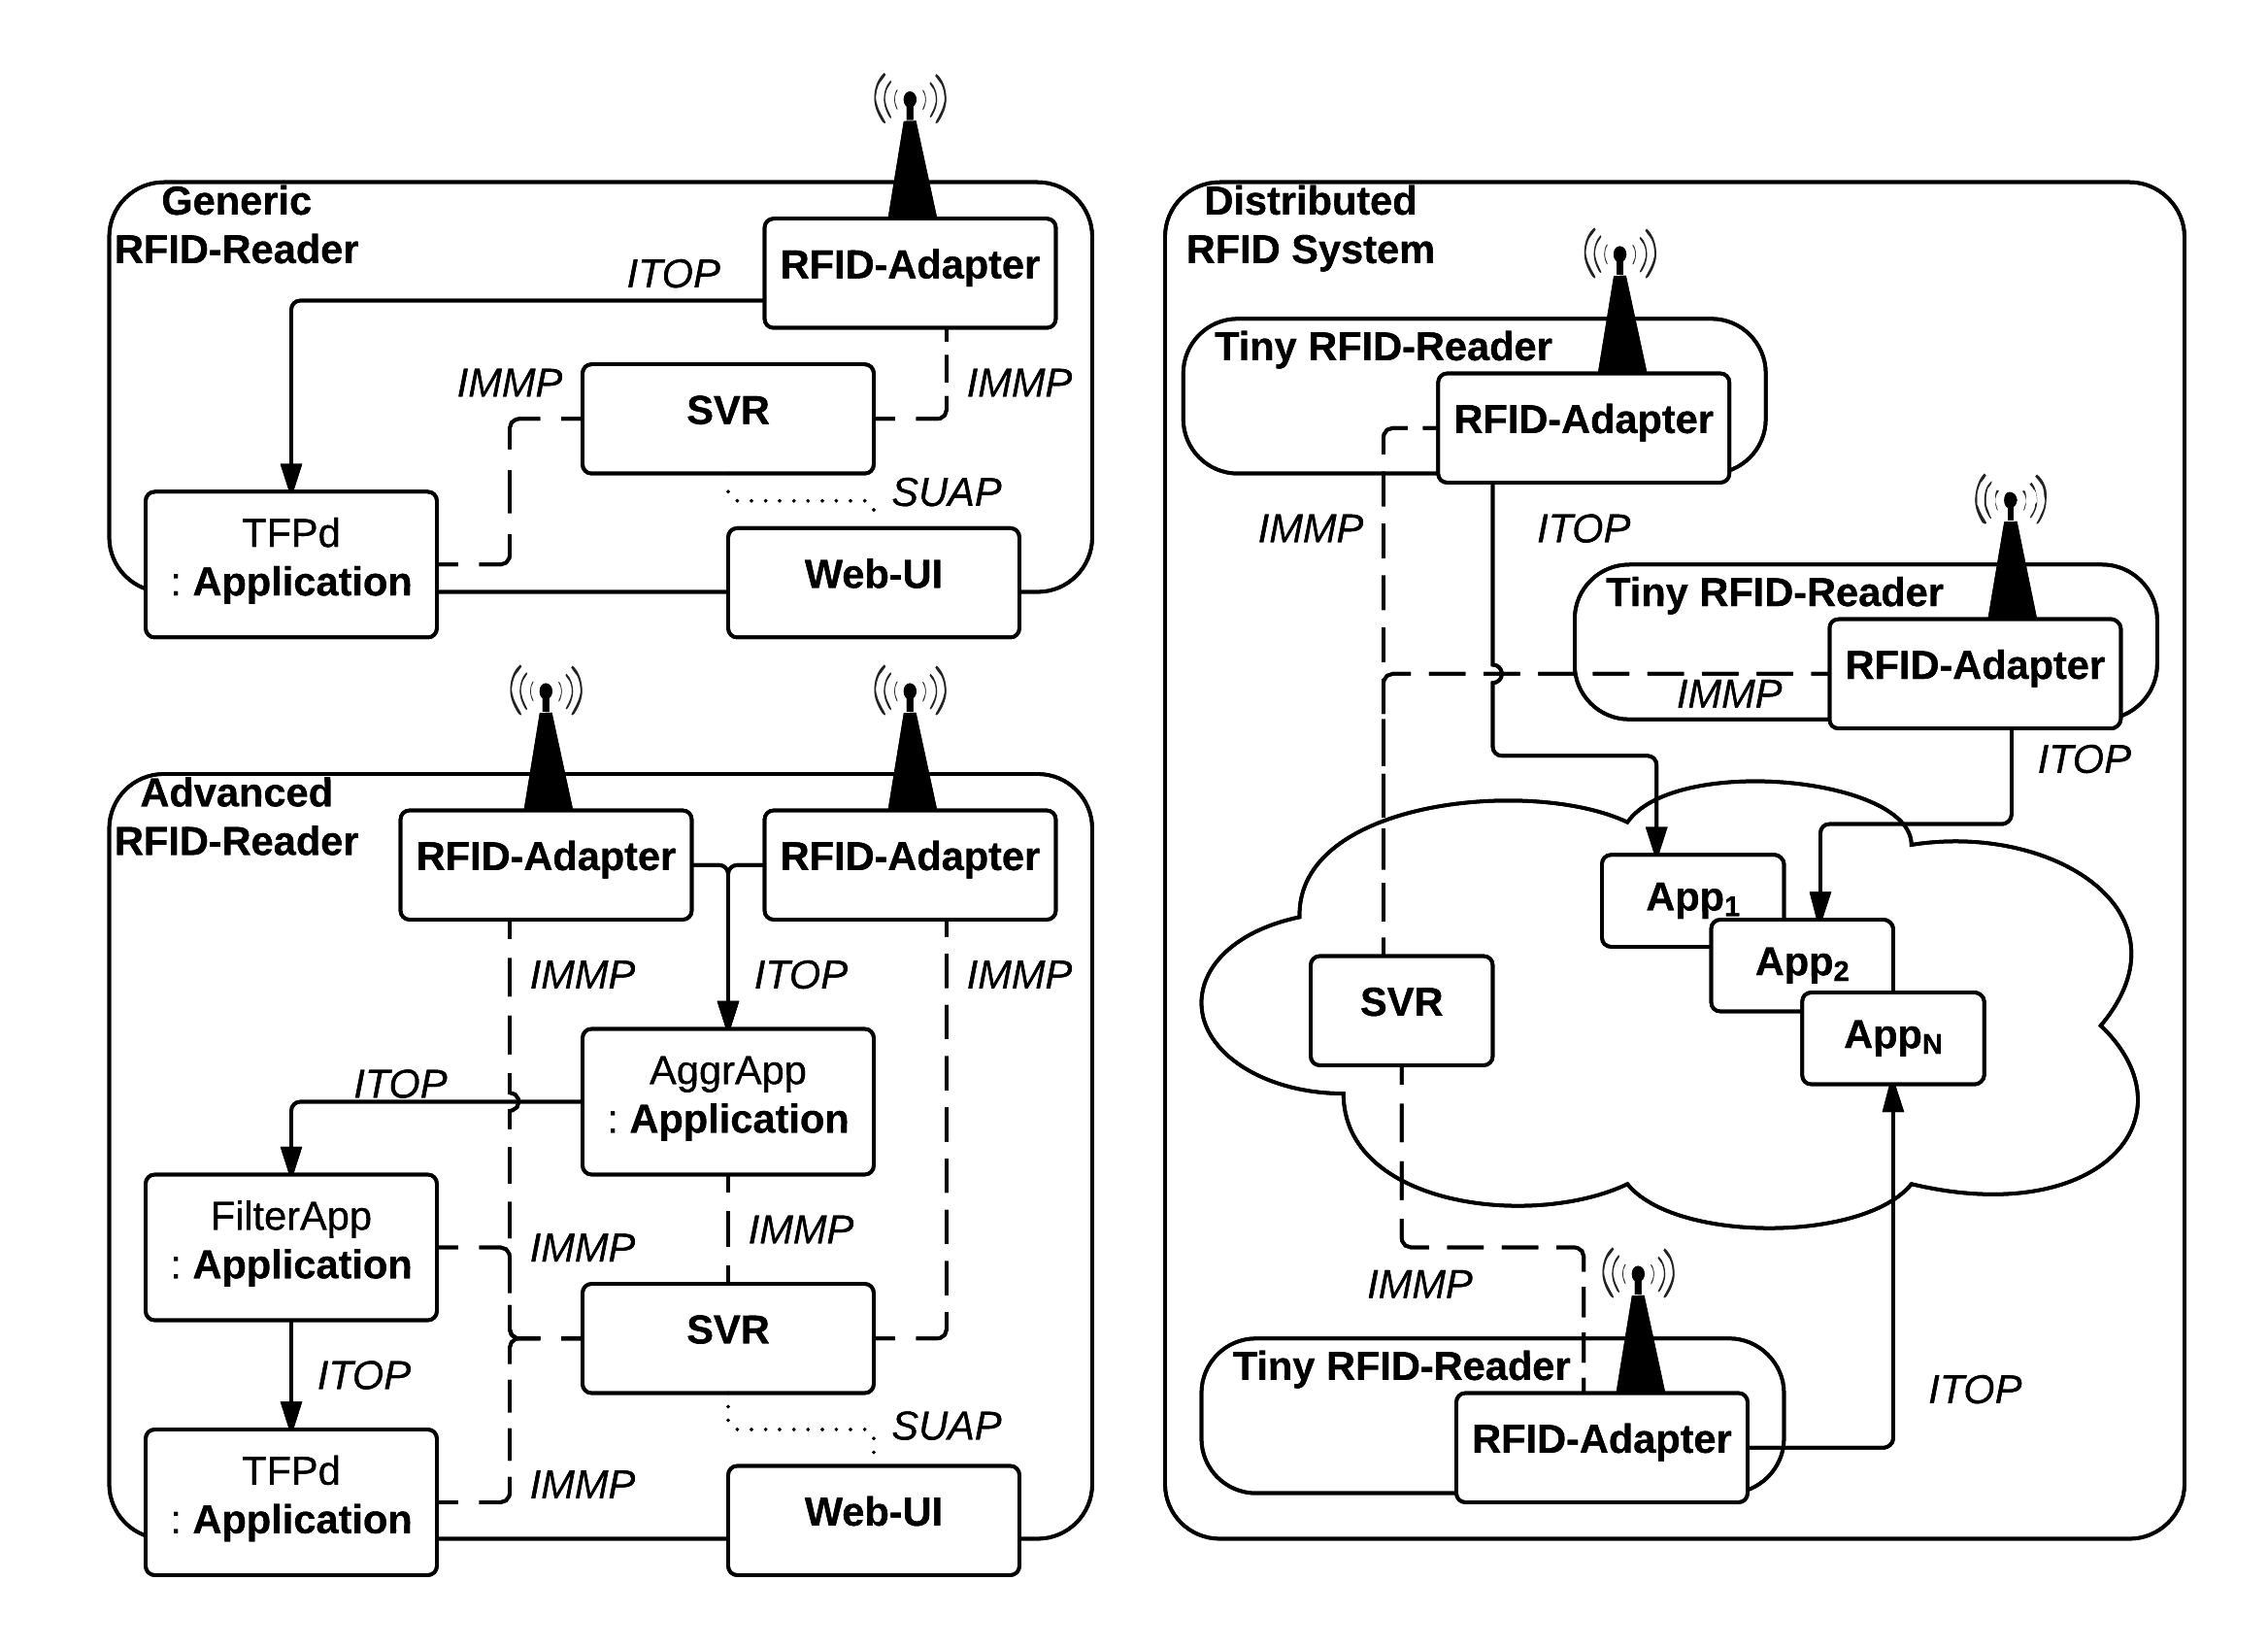
\includegraphics [width=0.9\textwidth]{chapter5/ch5_deployment_example}
  }
  \caption{Пример размещения компонентов системы}
  \label{fig:ch5_deployment_example}
\end{figure}

Поскольку все компоненты системы взаимодействуют друг с другом по сети, физически они могут располагаться где угодно. Типичные примеры размещений модулей по считывателям и серверам показаны на рис.~\ref{fig:ch5_deployment_example}.

Для обычного RFID--считывателя, построенного на базе среднего процессора (например, одноядерный ARM A7 или ARM A8), обладающего небольшим объемом оперативной памяти порядка 256--512~МБ и имеющего в составе один радиомодуль, достаточно установить SVR, RFID-адаптер, а также приложение для подключения к потоку прочитанных меток снаружи (TFPd) и модуль, предоставляющий доступ к настройке считывателю через web-интерфейс или консоль. Такое размещение компонентов позволяет передавать данные о всех прочитанных метках в центр обработки данных и, при необходимости, реализовывать операции чтения/записи через подключение внешних модулей и пользователей по протоколам ITOP и SUAP. Именно такая конфигурация считывателей использовалась в эксперименте, проведенном в городе Казань.

Если считыватель имеет более мощное вычислительное ядро, на нём также можно разместить несколько приложений (например, для фильтрации прочитанных меток или объединения с данными, получаемыми от другого считывателя). Если считыватель включает несколько радиомодулей, то также потребуется размещение несольких RFID--адаптеров. Хотя каждый компонент системы не требователен к вычислительным ресурсам по отдельности, для выполнения задач обработки поток меток могут потребоваться дополнительные ресурсы. Желательно использовать 2-х или 4-х ядерный процессор ARM и 512 "--- 1024 МБ оперативной памяти.

В наиболее сложном случае система может работать в распределенном режиме, а различные ее компоненты размещаться на считывателях и серверах, при этом считыватели могут быть сделаны чрезвычайно <<тонкими>> "--- на них достаточно разместить RFID--адаптер, который будет подключаться по сети к SVR, работающему на внешнем сервере. Приложения также могут работать на отдельных физических или виртуальных внешних серверах. В этом варианте считыватели могут быть реализованы на самых простых вычислительных компонентах, что позволит снизить их стоимость. При этом приложения и SVR выполняются в центре обработки данных, на мощном вычислительном оборудовании, благодаря чему им можно поручить работу с большим числом считывателей и выполнение достаточно сложных функций. Такой вариант размещения наиболее гибок и позволяет построить распределенную систему, состоящую из сотен считывателей, каждый из которых может администрироваться из единой консоли администратора. Добавление нового считывателя реализуется просто: администратор должен прописать адрес SVR в настройках RFID--адаптера, а также настроить приложения на работу с этим считывателем.



%%%%%%%%%%%%%%%%%%%%%%%%%%%%%%%%%%%%%%%%%%%%%%%%%%%%%%%%%%%%%%%%%%%%%%%%%%%%%%%%
\section{Протоколы взаимодействия компонентов системы}\label{sec:ch5_protocols}
%%%%%%%%%%%%%%%%%%%%%%%%%%%%%%%%%%%%%%%%%%%%%%%%%%%%%%%%%%%%%%%%%%%%%%%%%%%%%%%%

Для работы распределенной системы были разработаны четыре протокола:

\begin{itemize}
\item{\textit{IMMP} (\textit{Internal Modules Management Protocol}): протокол, используемый компонентами системы для подключения к SVR. Позволяет передавать начальную конфигурацию модулям, предоставляет возможность получения и установки значений объектам--параметрам и обеспечивает возможность вызова объектов--процедур. Протокол работает поверх TCP.}
\item{\textit{SUAP} (\textit{Simple User Access Protocol}): подключает пользователей к SVR, предоставляет возможность получения и установки значений параметров и удаленного вызова процедур. Работает через UDP.}
\item{\textit{ITOP} (\textit{Internal Tags Operation Protocol}): предоставляет соединения между компонентами для передачи данных о считанных метках, а также позволяет записывать метки и выполнять с ними прочие операции. Содержит механизмы для подписывания на поток считанных меток.}
\item{\textit{TFP} (\textit{Tag Flow Protocol}): упрощенная версия ITOP, предоставляющая возможность создания подписки на поток считанных меток. Может использоваться для подключения внешних приложений "--- например, клиента, записывающего поток меток в базу данных или клиента, записывающего данные во внутренний кэш для последующей выгрузки во внешние базы.}
\end{itemize}

Все протоколы имеют клиент--серверную архитектуру, соединение создаётся клиентом. Каждый запрос должен подтверждаться получателем с помощью специального сообщения \texttt{Response}, содержащего результат обработки запроса или код ошибки. Запросы упорядочиваются с помощью порядкового номера \texttt{ReqSN} (Request Sequence Number): клиент и сервер поддерживают по счетчику, перед отправкой значение счетчика увеличивается и помещается в соответствующее поле в запросе. В ответе на запрос поле \texttt{ReqSN} должно совпадать со значением счетчика из запроса. Этот механизм позволяет реализовать асинхронную обработку запросов "--- отправителю запроса не нужно ждать ответа для того, чтобы передать новый запрос. При этом отправитель может быть уверен, что запросы будут обработаны в порядке их передачи: если получатель видит, что номер запроса меньше последнего обработанного, запрос будет проигнорирован. С каждым запросом также связано максимальное ожидание ответа, после которого отправитель считает, что запрос не был выполнен.

Формат сообщений, кодируемых с помощью ASCII-строк, аналогичен форматам, используемым в HTTP v1.1 и SIP.


%%% --------------------------------------------
\subsection{Протокол управления платформой (IMMP)}\label{sec:ch5_immp}
%%% --------------------------------------------

\begin{figure}[ht] 
  \centerfloat{
    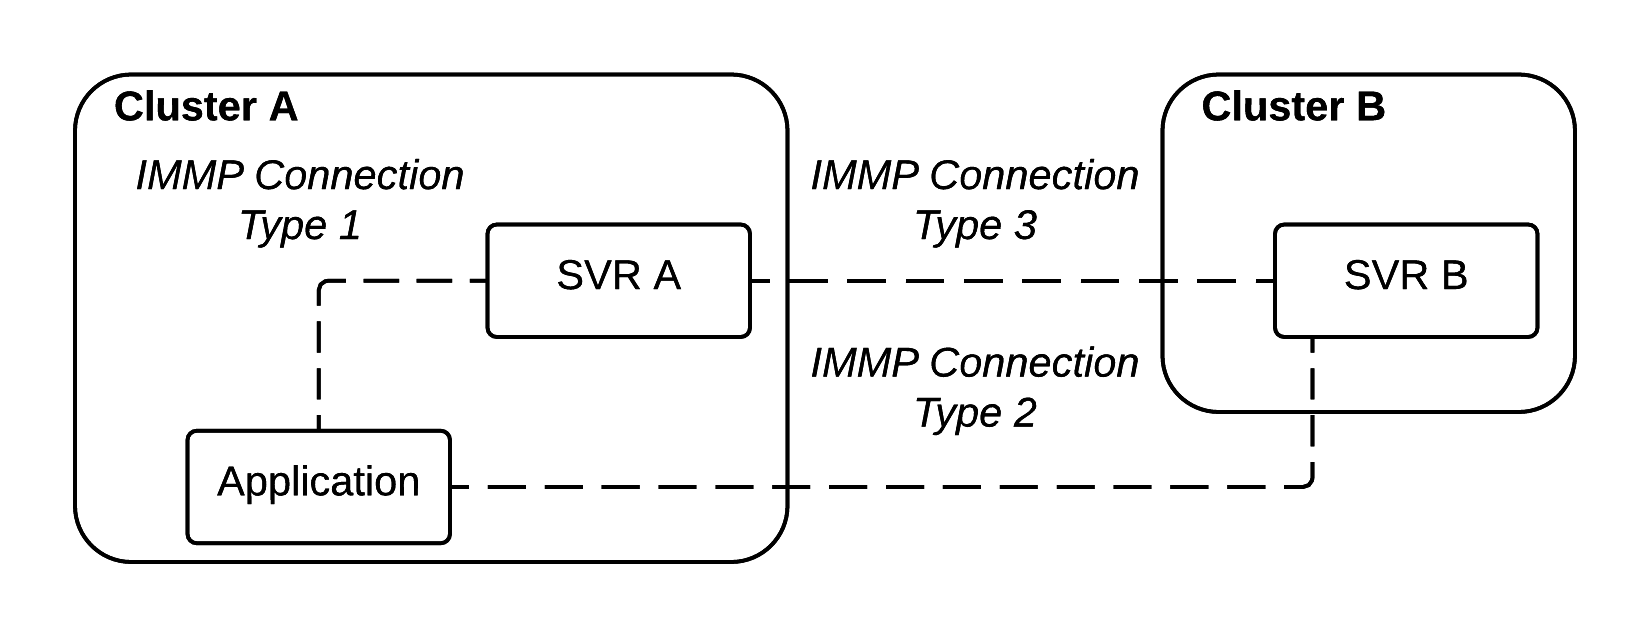
\includegraphics [width=0.8\textwidth] {chapter5/ch5_immp_connections}
  }
  \caption{Примеры IMMP-соединений}
  \label{fig:ch5_immp_connections}
\end{figure}

Протокол IMMP работает поверх транспортного уровня TCP и реализует функции получения модулями своей начальной конфигурации от супервайзера, поиск IP-адреса модуля по имени (сервис локации), получение и установка значений объектов, а также удалённый вызов процедур. В рамках IMMP различаются три типа соединений (см. рис.~\ref{fig:ch5_immp_connections}):

\begin{itemize}
	\item Тип 1: соединения между модулем с SVR из того же кластера. В этом соединении могут передаваться любые запросы, получение стартовой конфигурации модулем осуществляется через это соединение. В роли клиента всегда выступает модуль, подключаемый к SVR.
	\item Тип 2: соединения между модулем с SVR из другого кластера. Схоже с соединением типа 1, но не предполагает передачу стартовой конфигурации и может содержать ограничения на установку значений параметров и вызов процедур. Как и в соединении типа 1, в роли клиента всегда выступает модуль, подключаемый к SVR.
	\item Тип 3: соединения между SVR из разных кластеров. Предназначен для настройки SVR-клиента, инициализирующего соединение, через SVR--сервер. Предполагается, что SVR может поддерживать не более одного соединения типа 3 в качестве клиента, и сколько угодно --- в качестве сервера.
\end{itemize}

В протоколе определены семь запросов: \texttt{HELLO}, \texttt{ACK}, \texttt{BYE}, \texttt{LOCATE}, \texttt{GET}, \texttt{SET} и \texttt{CALL}. Запрос \texttt{HELLO} отправляется клиентом для создания соединения. Если соединение может быть установлено, сервер (SVR) сначала передает \texttt{Response} с кодом успеха (200), а затем "--- запрос \texttt{ACK}, в котором передает параметры сессии, включая ключ сессии \texttt{SKey} (Session Key). Запрос \texttt{LOCATE} используется для поиска компонентов по их именам или типам. Запросы \texttt{GET} и \texttt{SET} используются для чтения и записи значений объектов--параметров, а запрос \texttt{CALL} "--- для удаленного вызова процедур. Запросы \texttt{GET}, \texttt{SET} и \texttt{CALL} могут передаваться как клиентом, так и сервером.

\begin{figure}[ht] 
  \centering
  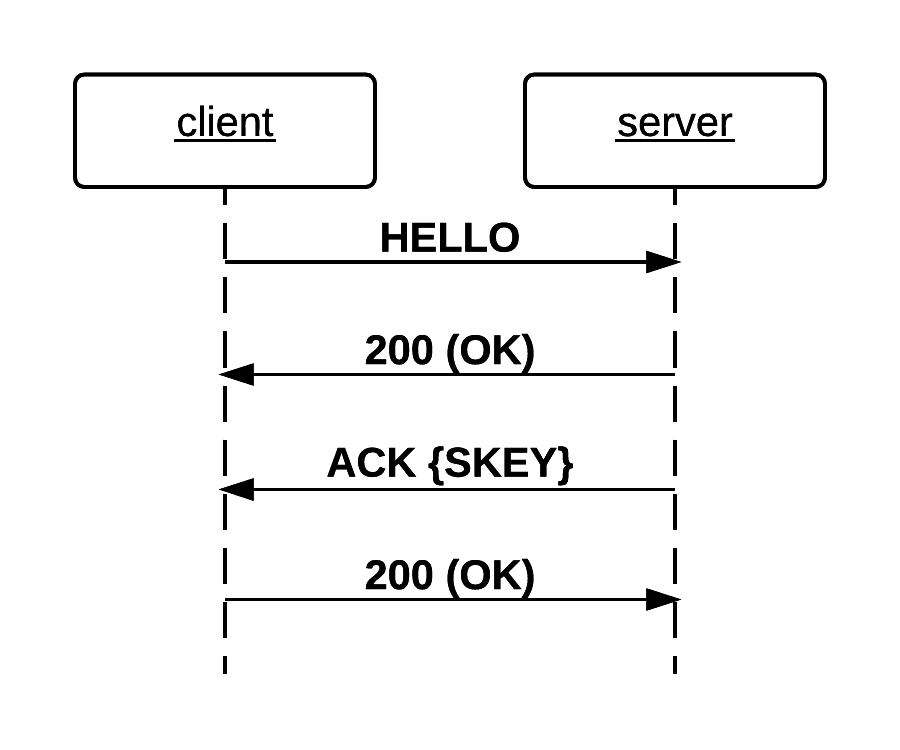
\includegraphics [width=0.4\textwidth] {chapter5/ch5_immp_session_establishment}
  \caption{Создание IMMP-соединения}
  \label{fig:ch5_immp_session_establishment}
\end{figure}

Создание соединения показано на рис.~\ref{fig:ch5_immp_session_establishment}. Клиент передает запрос \texttt{HELLO} со своим типом и именем. Сервер передает ответ \texttt{Response} с кодом 200. Затем сервер готовит стартовую конфигурацию клиента и передает ее в запросе \texttt{ACK}, получение которого также должен подтвердить клиент отправкой \texttt{Response}. Такое разделение ответов сервера возникает из-за того, что при высокой нагрузке на SVR подготовка стартовой конфигурации может занять время, которое может превышать время ожидания ответа на запрос \texttt{HELLO}. После получения ответа на \texttt{HELLO} клиент может ждать гораздо дольше получения своей конфигурации в \texttt{ACK}. Помимо начальной конфигурации, в \texttt{ACK} супервайзер передает ключ сессии \texttt{SKey}, который используется в дальнейшем обмене сообщениями. Хотя при использовании постоянных соединений TCP этот ключ представляет собой скорее рудимент, в будущем предполагается возможность использования на транспортном уровне протокола UDP, а в этом случае использование ключа позволяет идентифицировать запрос с сеансом.

Если одному компоненту нужен адрес другого компонента (например, для создания ITOP-соединения), он передает запрос \texttt{LOCATE} своему SVR. Если компонент найден, SVR передает его адрес в ответе на \texttt{LOCATE}. Если SVR не может найти компонент среди своих подключений, он может передать запрос по соединениям типа 3 для поиска компонента в других кластерах.

Если SVR нужно выполнить какую-либо операцию над объектом другого компонента, он передает соответствующий запрос (\texttt{GET}, \texttt{SET} или \texttt{CALL}). Если же компоненту A нужно выполнить действие над объектом компонента B, то SVR выступает в роли прокси-сервера: компонент A передает запрос SVR, который SVR передает компоненту B, дожидается ответа и пересылает его компоненту A.

Одно из приемуществ использования IMMP для управления компонентами системы "--- возможность быстрого изменения расположения компонентов. Если приложению нужно установить соединение, например, с RFID-адаптером, он запрашивает его адрес с помощью запроса \texttt{LOCATE}, в котором использует символьное имя этого адаптера (или, если ему нужно подключиться ко всем адаптерам, достаточно указать тип). В ответе SVR сообщит адрес (или адреса), по которым приложение уже может подключаться к адаптерам.



%%% --------------------------------------------
\subsection{Протокол подключения интерфейсов управления (SUAP)}\label{sec:ch5_suap}
%%% --------------------------------------------

Протокол SUAP представляет собой упрощенную версию IMMP, работающую через UDP. Он предназначен для подключения пользовательских интерфейсов к SVR. В функции SUAP входят получение и установка значений параметров, удаленный вызов процедур и обнаружение компонентов. Предполагается, что модули, предоставляющие пользователям доступ, не имеют своих объектов, поэтому передавать им начальную конфигурацию не надо, соответственно, отсутствует запрос \texttt{ACK}. По этой же причине протокол не является симметричным "--- запросы \texttt{GET}, \texttt{SET} и \texttt{CALL} могут передаваться только от клиента серверу. Ключ сессии \texttt{SKey} необходим для идентификации клиента и сессии и, ввиду отсутствия \texttt{ACK}, передается SVR клиенту в ответе на запрос \texttt{HELLO}.

Так как SUAP работает через UDP, в нем присутствует механизм для отслеживания состояния соединений: если сервер не получает от клиента ни одного сообщения в течение определенного интервала (по-умолчанию, 10 минут), он считает, что клиент отключился и сессия завершается. Для предотвращения этой ситуации, клиент может периодически передавать специальные короткие запросы \texttt{KEEPALIVE}, если передавать содержательные запросы ему не нужно.



%%% --------------------------------------------
\subsection{Протокол работы с RFID-адаптерами (ITOP)}\label{sec:ch5_itop}
%%% --------------------------------------------

Протокол предназначен для связи между компонентами системы (приложениями и RFID-адаптерами), желающими осуществлять действия над метками. Он позволяет читать и записывать память меток, а также подписываться на потоки считанных меток. Подписка может быть позднее отменена, также она завершается при закрытии соединения любой из сторон.

В протоколе определены семь запросов: \texttt{HELLO}, \texttt{READMEM}, \texttt{WRITEMEM}, \texttt{WRITEEPC}, \texttt{SUBSCRIBE}, \texttt{UNSUBSCRIBE} и \texttt{BYE}. Запросы \texttt{HELLO} и \texttt{BYE} используются для создания и завершения соединений соответственно, причем запрос \texttt{HELLO} может передаваться только клиентом, а \texttt{BYE} "--- любой из сторон. \texttt{SUBSCRIBE} и \texttt{UNSUBSCRIBE} передаются клиентом и используются для создания и отмены подписки соответственно. Запросы \texttt{READMEM}, \texttt{WRITEMEM} и \texttt{WRITEEPC} передаются клиентом для чтения или записи данных на заданную метку.

В протоколе ITOP также определен специальный вид сообщения--ответа \texttt{NOTIFY}. Это сообщение асинхронно передаётся сервером для информирования клиента, подписавшегося на поток, о прочтении новой метки. Он содержит следующие поля:

\begin{itemize}
	\item \texttt{epc}: значение EPC прочитанной метки;
	\item \texttt{tid}: значение банка TID прочитанной метки;
	\item \texttt{um}: значение банка UserMemory прочитанной метки;
	\item \texttt{id}: значение идентификатора метки, определенного приложением;
	\item \texttt{rssi}: мощность принятого сигнала;
	\item \texttt{antenna}: номер антенны RFID-считывателя, на которой была считана метка;
	\item \texttt{source}: имя RFID-адаптера, который изначально считал метку;
	\item \texttt{count}: число раз, которое метка была считана.
\end{itemize}

Идентификатор \texttt{id} заполняется данными, специфичными для приложения. Оно может содержать значение EPC или некоторое значение, полученное приложением с помощью EPC, TID, UserMemory. Например, в роли идентификатора может выступать номер транспортного средства, полученный приложением посредством обращения к базе данных.

Когда клиент хочет установить ITOP-соединение, ему требуется обнаружить ITOP-сервер. Если клиент знает имя сервера, но не знает его IP-адрес, он передает запрос \texttt{LOCATE} на SVR через IMMP или SUAP и получает адрес сервера в ответе. Зная адрес, клиент создает с ним TCP-соединение и передает запрос \texttt{HELLO}. В запрос \texttt{HELLO} также включается значение \texttt{SKey}, полученный клиентом ранее, при создании IMMP- или SUAP--соединения. Значение \texttt{SKey} используется для авторизации сервером клиента на выполнение той или иной операции. Например, администраторы и наблюдатели не имеют права записывать метки, а единственная разрешенная им операция "--- создание подписки на получение потока меток.

\begin{figure}[ht] 
  \centerfloat{
    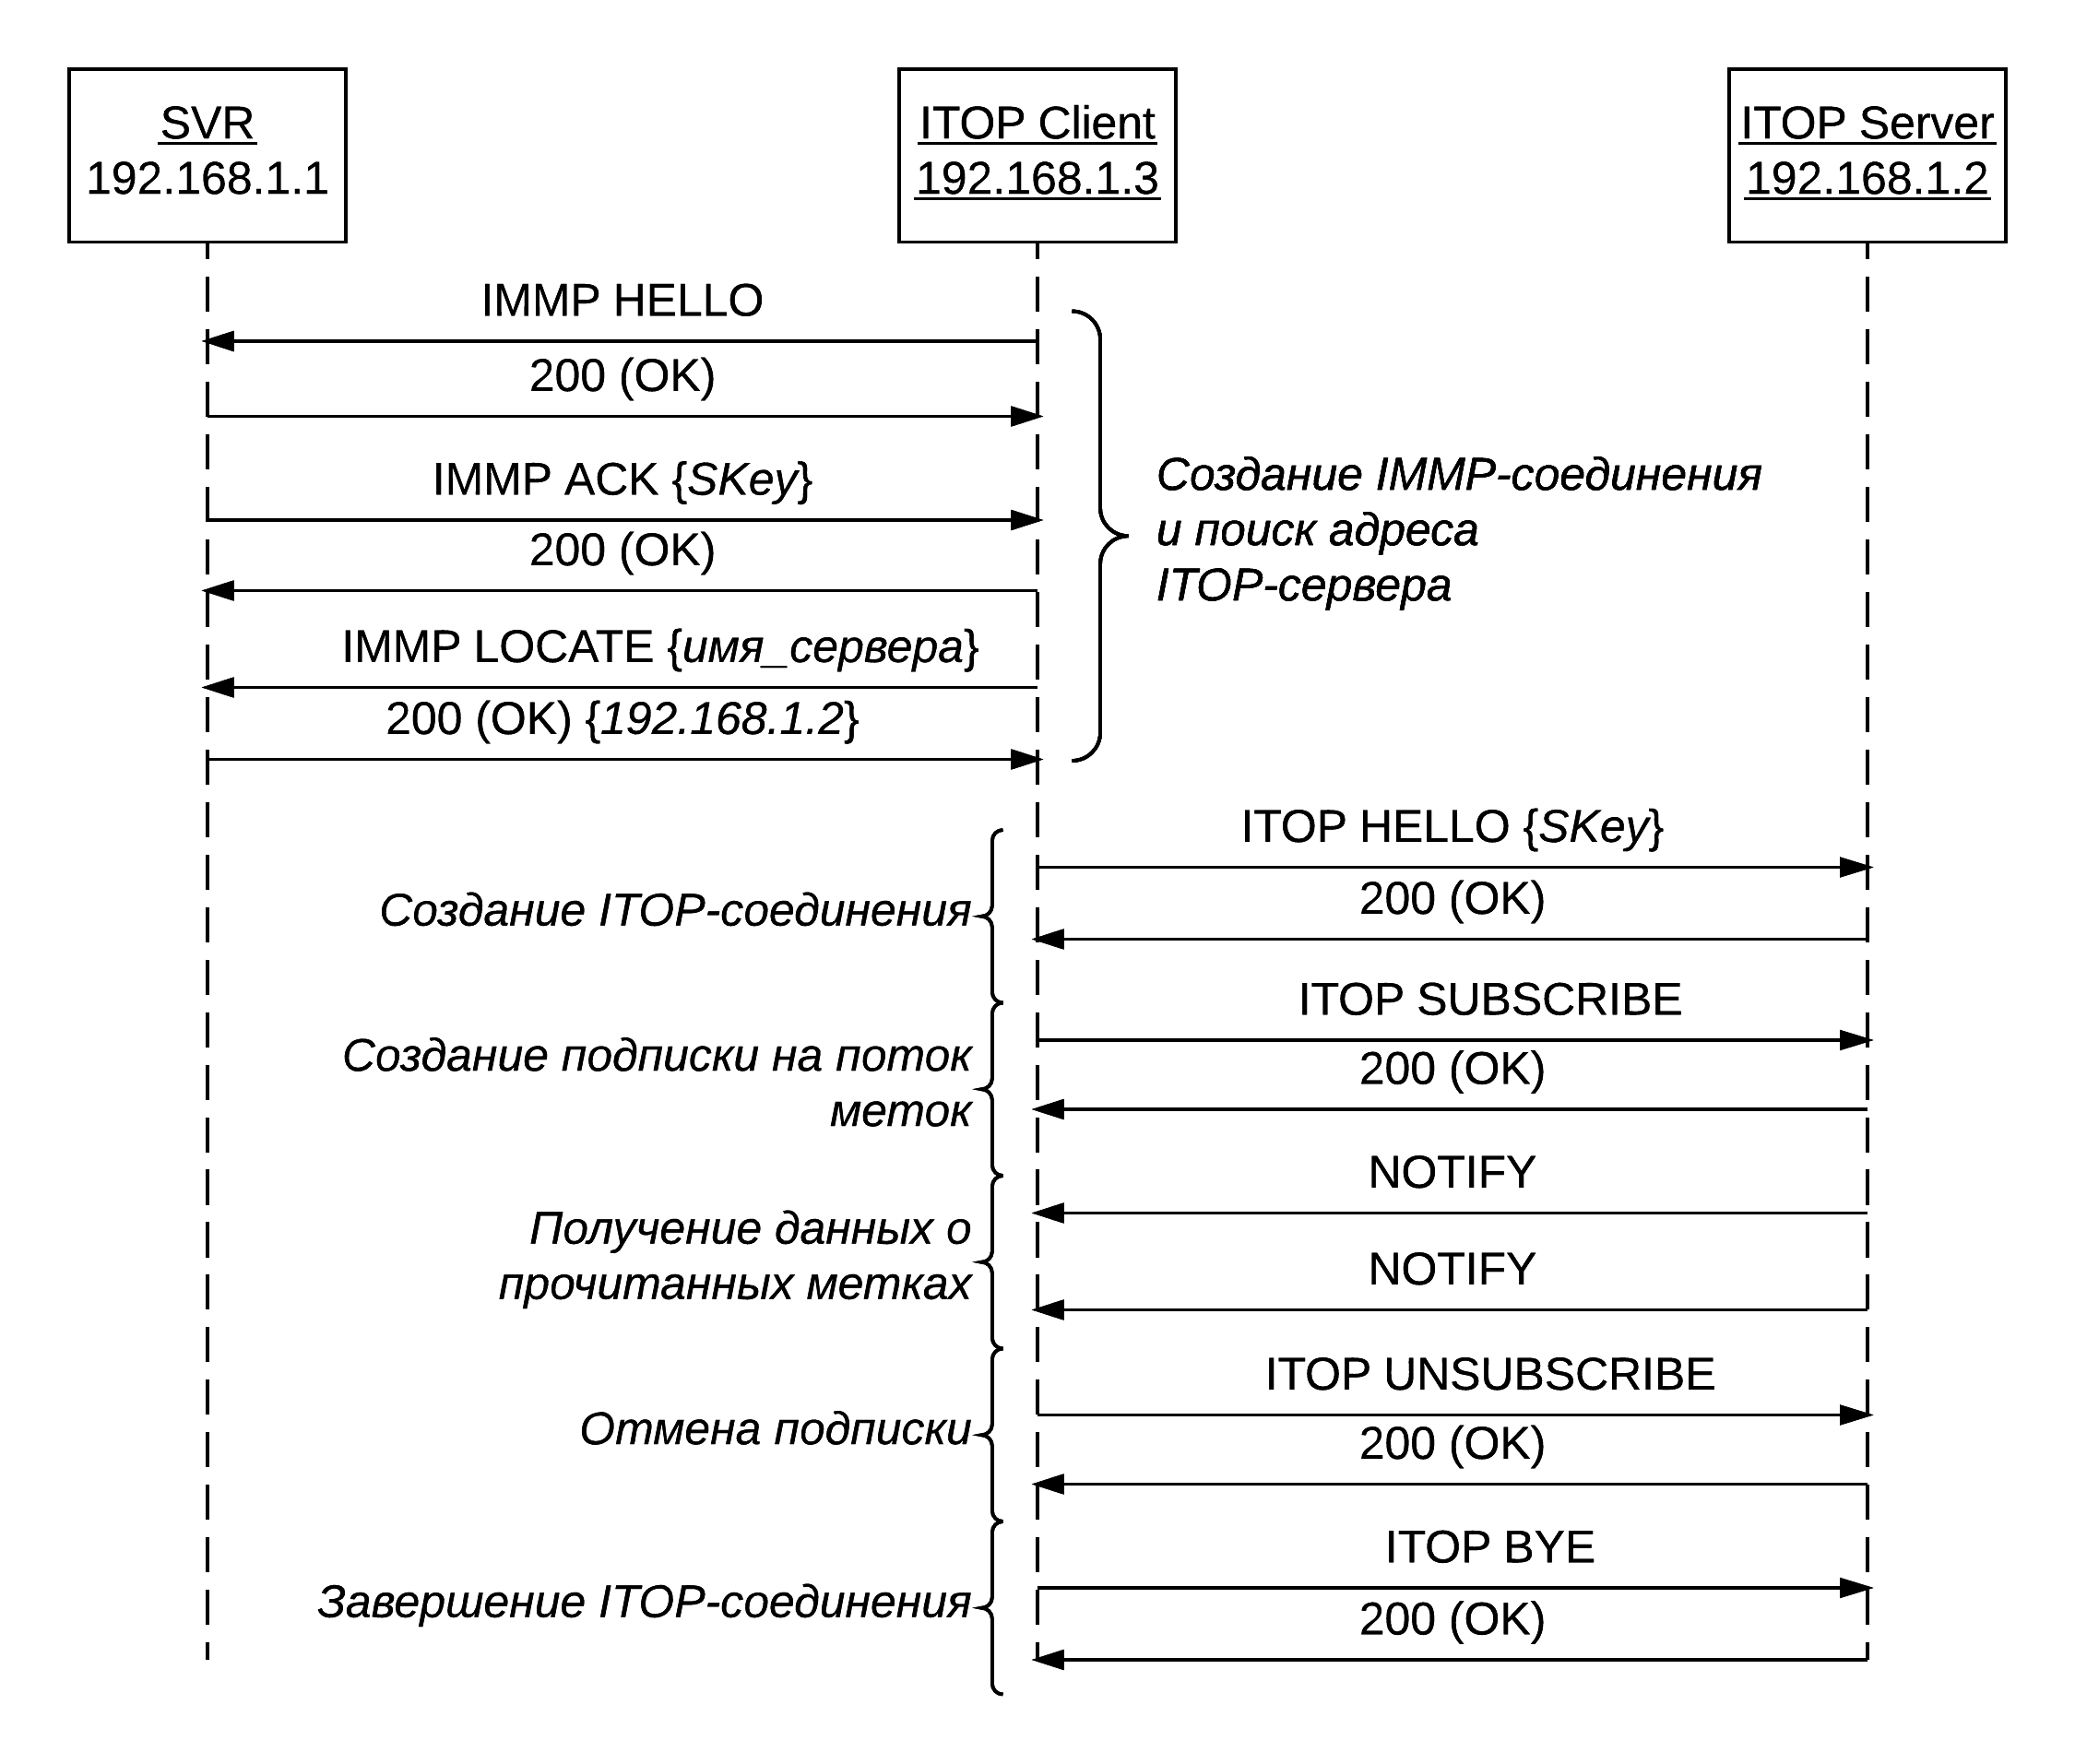
\includegraphics [width=0.8\textwidth] {chapter5/ch5_itop_session}
  }
  \legend{Клиент подключается по IMMP к SVR и получает ключ сессии \texttt{SKey}, затем запрашивает адрес ITOP-сервера. Получив адрес, клиент создает соединение с ITOP-сервером с использованием ключа \texttt{SKey}, создает подписку на получение меток. После получения двух меток клиент отменяет подписку и завершает соединение.}
  \caption{Пример ITOP-сессии}
  \label{fig:ch5_itop_session}
\end{figure}

Если клиент желает непрерывно получать информацию о прочитанных метках от сервера, он передает запрос \texttt{SUBSCRIBE}. Как только считывается (если сервер "--- RFID-адаптер) или принимается (если сервер "--- приложение) новая метка, сервер передает сообщение \texttt{NOTIFY} клиенту, содержащее информацию о метке. Когда клиент желает остановить получение потока, он отменяет подписку передачей запроса \texttt{UNSUBSCRIBE}. Пример сессии с показан на рис.~\ref{fig:ch5_itop_session}


%%% --------------------------------------------
\subsection{Протокол потокового чтения меток (TFP)}\label{sec:ch5_tfp}
%%% --------------------------------------------

Протокол TFP является упрощенной версией протокола ITOP и предназначен для получения данных о метках из пользовательских интерфейсов или внешних клиентов. Специальное приложение TFP Daemon (TFPd) реализует TFP-интерфейс и выступает в роли моста между ITOP и TFP: с одной стороны это приложение выступает в роли сервера протокола TFP, с другой "--- клиента ITOP. В протоколе TFP поддерживается только механизм создания подписок, прочие функции (запись меток, чтение заданных областей памяти и пр.) он не реализует. Кроме того, в сообщении \texttt{HELLO} не передается ключ сессии \texttt{SKey}, так как приложение TFPd использует свой собственный (системный) уровень доступа для создания ITOP-соединения с источником данных, позволяющий создавать подписки.



%%%%%%%%%%%%%%%%%%%%%%%%%%%%%%%%%%%%%%%%%%%%%%%%%%%%%%%%%%%%%%%%%%%%%%%%%%%%%%%%
\section{Приложения в программной платформе}\label{sec:ch5_applications}
%%%%%%%%%%%%%%%%%%%%%%%%%%%%%%%%%%%%%%%%%%%%%%%%%%%%%%%%%%%%%%%%%%%%%%%%%%%%%%%%

Кратко рассмотрим основные приложения, использующиеся в системе: агрегатор потоков AggrApp и TFP-сервер TFPd и кэш CacheApp. Работа этих приложений показана на рис.~\ref{fig:ch5_applications_scheme}.

\begin{figure}[ht] 
  \centerfloat{
    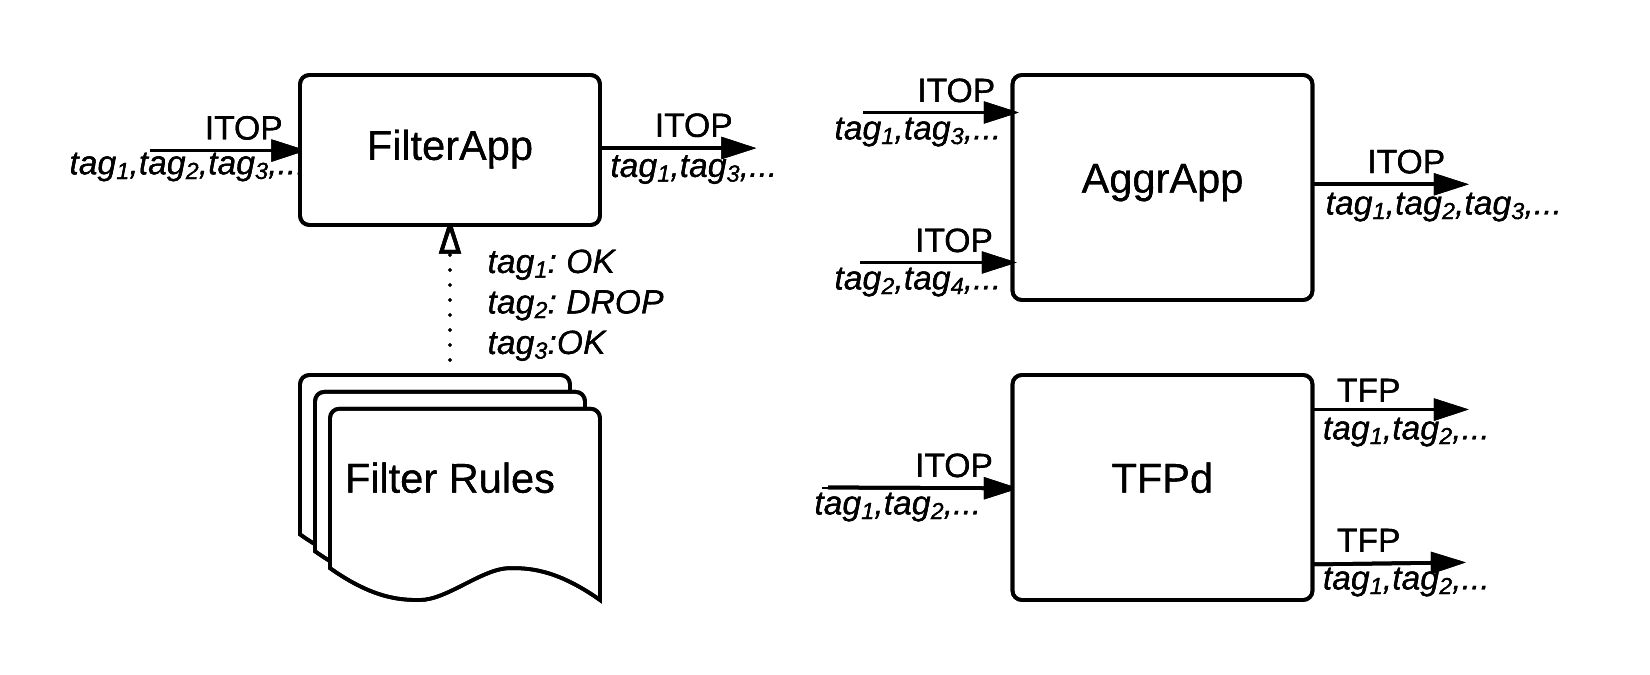
\includegraphics [width=0.85\textwidth] {chapter5/ch5_applications_scheme}
  }
  \caption{Приложения в программной платформе}
  \label{fig:ch5_applications_scheme}
\end{figure}

В дальнейшем могут быть реализованы более сложные приложения: фильтрация и модификация потока меток, преобразование протоколов (например, для подключения к платформе по протоколу web sockets), поиск номеров автомобилей по меткам в реальном времени и прочие.


%%% --------------------------------------------
\subsection{Агрегация потоков (AggrApp)}
%%% --------------------------------------------

Большинство приложений может подключаться к единственному ITOP-потоку. Если нужно объединить данные, поступающие от двух или более источников данных, можно использовать приложение AggrApp. Его функция "--- пересылка всем клиентам каждого \texttt{NOTIFY}-сообщения, поступающего в любом из входящих ITOP-соединений. Это единственное из приложений, имеющих множественный вход и множественный выход.

Приложение AggrApp создает подписки у своих источников данных только тогда, когда к нему подключается и создает подписку первый клиент. Если ни один клиент не подписан на поток от приложения, само приложение также не инициирует подписку.


%%% --------------------------------------------
\subsection{TFP-сервер и кэш}
%%% --------------------------------------------

Компоненты внутри системы используют протокол ITOP для чтения и записи меток. В то же время, для подключения внешних клиентов (например, для записи данных о проездах в базу данных в центре обработки данных) не нужны все функции ITOP. В частности, не нужно (и даже не желательно) иметь возможность записывать метки из ЦОДа. Для упрощения таких задач используется протокол TFP, который был рассмотрен ранее "--- в отличие от ITOP, он предоставляет возможность только для управления подпиской на поток данных о прочитанных метках.

Для того, чтобы преобразовать поток данных о прочитанных метках, получаемый от адаптеров или других приложений по протоколу ITOP, в TFP-поток, применяется приложение TFPd. При подключении первого клиента и создания этим клиентом подписки, TFPd связывается с источником данных по протоколу ITOP, подписывается на ITOP-поток и передает все \texttt{NOTIFY}-сообщения из ITOP-сессии в TFP-сессии. При отлючении последнего TFP-клиента подписка на ITOP-поток также отменяется.

Еще одно приложение, CacheApp, размещается обычно на том же оборудовании, на котором работает TFPd, и сохраняет в файл журнала все данные, полученные от него по протоколу TFP. Это приложение оказывается особенно полезным, когда и RFID-адаптер, и TFP-сервер расположены на считывателе, который связан с центром обработки данных плохим каналом связи и позволяет избежать потери данных о прочитанных метках.



%%%%%%%%%%%%%%%%%%%%%%%%%%%%%%%%%%%%%%%%%%%%%%%%%%%%%%%%%%%%%%%%%%%%%%%%%%%%%%%%
\section{Экспериментальная реализация системы}\label{sec:ch5_implementation}
%%%%%%%%%%%%%%%%%%%%%%%%%%%%%%%%%%%%%%%%%%%%%%%%%%%%%%%%%%%%%%%%%%%%%%%%%%%%%%%%

Все описанные программные модули и протоколы, кроме части RFID-адаптера, взаимодействующей со считывателем и веб-интерфейса, были реализованы на языке C++. Часть RFID-адаптера, работающая непосредственно с радиомодулем считывателя, была реализована на C. Для реализации web-интерфейса использовался фреймворк Flask на языке Python 3. Все компоненты системы работают под управлением операционной системы Linux.

Помимо перечисленных ранее, в системе присутствует специальное приложение (RRRd), осуществляющее запуск и остановку компонентов.

Следует выделить несколько особенностей, общих для всех модулей кроме веб-интерфейса, реализованного на Python. Во-первых, в реализациях очередей, клиентов и серверов практически не используется динамическая память (функции \texttt{malloc}/\texttt{free}, операторы \texttt{new}/\texttt{delete} и пр.). Вместо этого под каждое сообщение или очередь заранее статически выделяется область памяти, заведомо превышающая предельно допустимый размер хранимого объекта. Этот подход позволяет не только повысить производительность за счёт отсутствия работы с выделением и освобождением памяти, но и существенно повысить надёжность за счёт снижения вероятности появления ошибок утечки памяти или обращений к ранее освобождённой памяти. 
	
Во-вторых, большинство модулей, включающих серверы каких либо протоколов (IMMP, ITOP и пр.) имеют в своем составе очереди, с помощью которых обработка запросов от различных клиентов мультиплексируется и может осуществляться даже одним потоком. Опрос сокетов также производится мультиплексированием функцией \texttt{pselect}. Более подробно эта идея будет описана на примерах SVR и RFID-адаптеров далее.
	
В-третьих, все модули реализованы в виде многопоточных приложений с использованием библиотеки pthreads (POSIX Threads).

Наибольшую сложность при разработке системы представляли супервайзер (SVR) и RFID-адаптер, поэтому в следующих разделах они рассмотрены подробнее.



%%% --------------------------------------------
\subsection{Реализация супервайзера}
%%% --------------------------------------------

В состав SVR входит очередь (управляется отдельным потоком), множество потоков-рабочих и поток-сервер.

\textbf{Поток-сервер} осуществляет запуск и остановку других потоков, взаимодействует с RRRd, а также выполняет роль сервера протоколов SUAP и IMMP. При запуске он открывает серверные сокеты протоколов SUAP и IMMP, создаёт TCP-сессии протокола IMMP по мере поступления запросов на соединения. Опрос сокетов производится методом мультиплексирования с помощью функции \texttt{pselect}. При получении сообщения протокола SUAP или IMMP поток-сервер создаёт событие и записывает его в очередь.

\textbf{Поток управления очередью} осуществляет помещение и извлечение событий из очереди, а также отслеживает директивные сроки каждого события. При истечении срока события оно извлекается из очереди, а в сессии IMMP или клиенту SUAP передается ответ с кодом ошибки, соответствующему истечению времени ожидания. Это позволяет своевременно оповещать клиентов о перегрузке системы и не тратить вычислительные ресурсы на обработку событий, которые с большой вероятностью уже не актуальны для клиента.

\textbf{Потоки-рабочие} осуществляют обработку событий. Например, если в событии содержится запрос на получение значения объекта, хранимого в другом модуле, рабочий произведёт обращение по протоколу IMMP к соответствующему модулю и, получив ответ, передаст его тому модулю, который инициировал запрос. Количество рабочих настраивается и, в зависимости от того, сколько модулей обслуживает SVR, может меняться от 1-2 до 10 и более, тем самым обеспечивая масштабирование системы в зависимости от нагрузки, а также используемой аппаратной платформы. Следует отметить, что слишком мало потоков-рабочих не следует делать даже на одноядерных системах, поскольку при обработке запросов им часто приходится ожидать ответов в течение времени, превышающего время активной обработки события.


%%% --------------------------------------------
\subsection{Реализация адаптера RFID}
%%% --------------------------------------------

Особенностью этого модуля является необходимость использования программного интерфейса радиомодуля, написанного на языке C. Для того, чтобы иметь возможность быстрой замены модулей, была реализована промежуточная библиотека (также на языке C), реализующая основные функции: чтение метки в течение заданного временного интервала, запись значение EPCID на метку, запись значения в заданный банк памяти, получение и запись значения параметра модуля.

Хотя дизайн промежуточной библиотеки был сделан очень близким к операциям, предоставляемым API использованного радиомодуля, её несложно адаптировать к радиомодулям других производителей, при наличии соответствующей спецификации протокола взаимодействия или API.

Сам протокол ITOP предоставляет два вида операций чтения: потоковое и по запросу. Поскольку одновременно к адаптеру могут подключаться несколько модулей (например, TFPd и веб-интерфейс), нужно обеспечить мультиплексирование доступа к радиомодулю, играющего роль разделяемого ресурса, причём должен обеспечиваться доступ для одновременного потокового чтения и чтения по запросу. К тому же, необходимо обеспечить возможность настройки параметров радиомодуля даже в то время, когда он занят чтением меток. Для решения этой задачи в RFID-адаптере была построена \textbf{очередь событий}, которая заполнялась событиями в зависимости от наличия подписок и пришедших запросов по ITOP- или IMMP-соединениям. Всего было определено четыре основных события: чтение меток в течение интервала $T$, запись значения на метку, получение и установка значения параметра;

Каждое событие имеет приоритет, причём для операции чтения он самый низкий. Важной общей чертой всех событий является то, что их обработка требует ограниченного времени, то есть никакое из событий не может захватить адаптер на неопределённо долгий срок.

Если хотя бы один клиент по протоколу ITOP запросил потоковое чтение, то в очередь добавляется событие чтения. По его завершению данные о прочитанных метках передаются всем клиентам, запросившим чтение меток (как потоковое, так и не потоковое), а в очередь добавляется новое событие чтения с тем же интервалом времени. Если другой клиент запрашивал чтение в течение времени, большего используемого интервала $T$, или хотел прочесть дополнительные банки памяти, то вместо очереднго события чтения добавляется новое, содержащее параметры этого запроса. 

Если приходит запрос на получение или изменение параметра адаптера, или же на запись данных на метку, то для них создаются соответствующие события. Так как эти события имеют приоритет выше, чем чтение, то они выполнятся раньше, независимо от наличия запросов на потокове или обычное чтение. Как следствие, супервайзеру, как и другим модулям, требуется меньше потоков: в текущей модели все TCP-сессии постоянны, а передача запроса и получение ответа происходят синхронно, то есть рабочий ждет ответа на переданный запрос. Если бы операции чтения меток вытесняли операции чтения или записи параметров, рабочие потоки SVR были бы вынуждены подолгу ждать ответа, что неизбежно сказалось бы на работоспособности и масштабируемости всей системы.

Когда все клиенты, ранее подписавшиеся на получение данных о прочитанных метках в потоке, завершают свою подписку или отключаются, автоматическое добавление новых событий чтения также прекращается. Таким образом, при отсутствии модулей, подписанных на чтение меток, радиомодуль не используется, что, в частности, позволяет снизить энергопотребление и температуру считывателя.



%%%%%%%%%%%%%%%%%%%%%%%%%%%%%%%%%%%%%%%%%%%%%%%%%%%%%%%%%%%%%%%%%%%%%%%%%%%%%%%%
\section{Результаты эксперимента и их анализ}\label{sec:ch5_results}
%%%%%%%%%%%%%%%%%%%%%%%%%%%%%%%%%%%%%%%%%%%%%%%%%%%%%%%%%%%%%%%%%%%%%%%%%%%%%%%%

В конце осени 2014 года был запущен большой эксперимент в городе Казани (республика Татарстан). В ходе эксперимента номерами с радиометками были оснащены 740 автобусов и были оборудованы четыре точки радиочастотной идентификации. Оборудование для двух из них было разработано коллективом при активном участии автора (разработка программного обеспечения считывателей, системы управления; установка, настройка программ в ЦОДе и настройка считывателей; анализ полученных результатов и расчёт вероятности идентификации).

\fixme{Вставить картинку со схемой софта в эксперименте}

На считывателях были размещены супервайзеры (SVR), приложения TFPd и CacheApp, а также RFID-адаптеры. Сервер был размещен в центре обработки данных (ЦОД) ГИБДД города Казань, подключение к считывателям происходило посредством протокола TFP. Кроме того, на считывателях были размещены HTTP-серверы (NGINX) и реализованы web--интерфейсы для настройки и мониторинга. Подключение веб-интерфейсов к SVR осуществлялось по протоколу SUAP, а к адаптерам "--- по протоколу ITOP. На сервере в ЦОД был размещён клиент клиент TFP и база данных MySQL, в которую производилась запись прочитанных меток. 

Для каждой метки в базу данных записывались: время, идентификатор считывателя, значения EPC и TID, уровень сигнала от метки, число прочтений, номер антенны. Также в отдельной таблице хранились соответствия значений TID и номерных знаков, поэтому была возможность выгрузки информации о времени проезда автобусов напрямую из базы данных.

\fixme{Вставить пример схемы таблиц и пример SELECT-запроса}

Эксперимент длился до начала 2015 года, в течение поздней осени и зимы. Задачей эксперимента было практически обосновать применимость технологии радиочастотной идентификации для регистрации проездов автомобилей на нормальных скоростях, в условиях городского потока, при плохих погодных условиях. 

\fixme{Вставить таблицу с параметрами, использованными на считывателях в Казани}

Считыватели были настроены на использование Tari=12.5~мкс, M=4, расширенные преамбулы не использовались. 

Для оценки вероятности идентификации, на протяжении нескольких дней силами ГИБДД Казани были собраны данные о проездах автобусов, с помощью визуального наблюдения. Эти данные были обработаны и произведено сравнение с информацией, полученной от считывателей, с поправкой на погрешности (например, время могло немного отличаться). Результаты несколько различались между точками и составили от 92~\% идентифицированных транспортных средств до 96~\%. 

Следует отметить, что одной из основных проблем при проведении эксперимента оказалась высокая перегруженность оптических каналов связи между считывателями и центром обработки данных, которые также использовались для передачи уличного видео наблюдения. Перегрузки приводили к тому, что значительную часть времени соединений между считывателями и сервером не было, но за счет использования кэширования удалось избежать потери данных о проездах. В то же время, для реального использования системы радиочастотной идентификации и обеспечения оперативного воздействия при обнаружении нарушений правил дорожного движения или, например, выявления похищенных автомобилей может требоваться либо предоставление гарантированной пропускной способности в существующих проводных каналах, либо построение беспроводных многошаговых сетей. Как было показано в главе 4 и, в частности, в работе \cite{WINET_DCCN2018}, для этой цели можно использовать даже самое простое и доступное оборудование стандарта IEEE 802.11g.





\clearpage
           % Глава 5
\chapter*{Заключение}                       % Заголовок
\addcontentsline{toc}{chapter}{Заключение}  % Добавляем его в оглавление

%% Согласно ГОСТ Р 7.0.11-2011:
%% 5.3.3 В заключении диссертации излагают итоги выполненного исследования, рекомендации, перспективы дальнейшей разработки темы.
%% 9.2.3 В заключении автореферата диссертации излагают итоги данного исследования, рекомендации и перспективы дальнейшей разработки темы.
%% Поэтому имеет смысл сделать эту часть общей и загрузить из одного файла в автореферат и в диссертацию:

Основные результаты работы заключаются в следующем.
%% Согласно ГОСТ Р 7.0.11-2011:
%% 5.3.3 В заключении диссертации излагают итоги выполненного исследования, рекомендации, перспективы дальнейшей разработки темы.
%% 9.2.3 В заключении автореферата диссертации излагают итоги данного исследования, рекомендации и перспективы дальнейшей разработки темы.
\begin{enumerate}
  \item Описан способ построения распределенной системы радиочастотной идентификации автомобилей, выделены факторы, влияющие на производительность системы;
  \item Представлены результаты численного исследования аналитической модели протокола EPC Gen2, показывающие целесообразность периодической смены считывателем опрашиваемого значения флага сессии и периодического сброса питания;
  \item Предложена имитационная модель системы радиочастотной идентификации автомобилей, учитывающая особенности распространения сигнала вблизи дороги, эффект Допплера, параметры антенных систем, настройки протокола EPC Gen.2;
  \item С помощью имитационного моделирования получены численные оценки вероятности идентификации быстро движущихся автомобилей при различных настройках протокола. Полученные результаты близко соотносятся с данными, полученными в ходе экспериментального внедрения системы, и показывают, что при определенных настройках можно добиться высокой вероятности идентификации быстро движущихся автомобилей с размещенными в номерных знаках метках;
  \item Описан способ построения распределений фазового типа для моделирования беспроводных каналов связи с использованием существующих стохастических моделей каналов;
  \item Предложена открытая сеть массового обслуживания с марковскими входными потоками, обслуживанием фазового типа и ограниченной памятью, повторными передачами и потерями пакетов из-за ошибок в канале, позволяющая моделировать беспроводную опорную сеть;
  \item Для беспроводных сетей с линейной топологией предложен метод оценки производительности с использованием систем массового обслуживания MAP/PH/1/n;
  \item Рассмотрен способ расчёта параметров производительности тандемных сетей массового обслуживания с узлами вида MAP/PH/1/n, позволяющий ограничить размерность модели за счет использования методов аппроксимации MAP-потоков обслуженных пакетов;
  \item Представлены численные результаты, показывающие адекватную точность предложенных методов моделирования беспроводных каналов связи и опорных беспроводных сетей с линейной топологией;
  \item Предложена архитектура промежуточного программного обеспечения для подключения большого количества географически разделенных RFID-считывателей к центру управления, обеспечивающего получение данных от считывателей, мониторинг и управление системой;
  \item Представлены результаты экспериментов по исследованию и внедрению системы радиочастотной иденификации автобусов в городе Казань 2014 и 2020 годов. Показано, что эффективность системы достигает 95~\%.
\end{enumerate}

И какая-нибудь заключающая фраза.

\fixme{Последний параграф может включать благодарности.  В заключение автор
выражает благодарность и большую признательность научному руководителю
Иванову~И.\,И. за поддержку, помощь, обсуждение результатов и~научное
руководство. Также автор благодарит Сидорова~А.\,А. и~Петрова~Б.\,Б.
за помощь в~работе с~образцами, Рабиновича~В.\,В. за предоставленные
образцы и~обсуждение результатов, Занудятину~Г.\,Г. и авторов шаблона
*Russian-Phd-LaTeX-Dissertation-Template* за~помощь в оформлении
диссертации. Автор также благодарит много разных людей
и~всех, кто сделал настоящую работу автора возможной.}
      % Заключение
\include{Dissertation/acronyms}        % Список сокращений и условных обозначений
\include{Dissertation/dictionary}      % Словарь терминов
\include{Dissertation/references}      % Список литературы
\include{Dissertation/lists}           % Списки таблиц и изображений (иллюстративный материал)

\setcounter{totalchapter}{\value{chapter}} % Подсчёт количества глав

%%% Настройки для приложений
\appendix
% Оформление заголовков приложений ближе к ГОСТ:
\setlength{\midchapskip}{20pt}
\renewcommand*{\afterchapternum}{\par\nobreak\vskip \midchapskip}
\renewcommand\thechapter{\Asbuk{chapter}} % Чтобы приложения русскими буквами нумеровались

% \chapter{Примеры вставки листингов программного кода}\label{app:A}

% Для крупных листингов есть два способа. Первый красивый, но в нём могут быть
% проблемы с поддержкой кириллицы (у вас может встречаться в~комментариях
% и~печатаемых сообщениях), он представлен на листинге~\cref{lst:hwbeauty}.
% \begin{ListingEnv}[!h]% настройки floating аналогичны окружению figure
%     \captiondelim{ } % разделитель идентификатора с номером от наименования
%     \caption{Программа ,,Hello, world`` на \protect\cpp}\label{lst:hwbeauty}
%     % окружение учитывает пробелы и табуляции и применяет их в сответсвии с настройками
%     \begin{lstlisting}[language={[ISO]C++}]
% 	#include <iostream>
% 	using namespace std;

% 	int main() //кириллица в комментариях при xelatex и lualatex имеет проблемы с пробелами
% 	{
% 		cout << "Hello, world" << endl; //latin letters in commentaries
% 		system("pause");
% 		return 0;
% 	}
%     \end{lstlisting}
% \end{ListingEnv}%
% Второй не~такой красивый, но без ограничений (см.~листинг~\cref{lst:hwplain}).
% \begin{ListingEnv}[!h]
%     \captiondelim{ } % разделитель идентификатора с номером от наименования
%     \caption{Программа ,,Hello, world`` без подсветки}\label{lst:hwplain}
%     \begin{Verb}

%         #include <iostream>
%         using namespace std;

%         int main() //кириллица в комментариях
%         {
%             cout << "Привет, мир" << endl;
%         }
%     \end{Verb}
% \end{ListingEnv}

% Можно использовать первый для вставки небольших фрагментов
% внутри текста, а второй для вставки полного
% кода в приложении, если таковое имеется.

% Если нужно вставить совсем короткий пример кода (одна или две строки),
% то~выделение  линейками и нумерация может смотреться чересчур громоздко.
% В таких случаях можно использовать окружения \texttt{lstlisting} или
% \texttt{Verb} без \texttt{ListingEnv}. Приведём такой пример
% с указанием языка программирования, отличного от~заданного по умолчанию:
% \begin{lstlisting}[language=Haskell]
% fibs = 0 : 1 : zipWith (+) fibs (tail fibs)
% \end{lstlisting}
% Такое решение "--- со вставкой нумерованных листингов покрупнее
% и~вставок без выделения для маленьких фрагментов "--- выбрано,
% например, в~книге Эндрю Таненбаума и Тодда Остина по архитектуре
% компьютера.

% Наконец, для оформления идентификаторов внутри строк
% (функция \lstinline{main} и~тому подобное) используется
% \texttt{lstinline} или, самое простое, моноширинный текст
% (\texttt{\textbackslash texttt}).

% Пример~\cref{lst:internal3}, иллюстрирующий подключение переопределённого
% языка. Может быть полезным, если подсветка кода работает криво. Без
% дополнительного окружения, с подписью и ссылкой, реализованной встроенным
% средством.
% \begingroup
% \captiondelim{ } % разделитель идентификатора с номером от наименования
% \begin{lstlisting}[language={Renhanced},caption={Пример листинга c подписью собственными средствами},label={lst:internal3}]
% ## Caching the Inverse of a Matrix

% ## Matrix inversion is usually a costly computation and there may be some
% ## benefit to caching the inverse of a matrix rather than compute it repeatedly
% ## This is a pair of functions that cache the inverse of a matrix.

% ## makeCacheMatrix creates a special "matrix" object that can cache its inverse

% makeCacheMatrix <- function(x = matrix()) {#кириллица в комментариях при xelatex и lualatex имеет проблемы с пробелами
%     i <- NULL
%     set <- function(y) {
%         x <<- y
%         i <<- NULL
%     }
%     get <- function() x
%     setSolved <- function(solve) i <<- solve
%     getSolved <- function() i
%     list(set = set, get = get,
%     setSolved = setSolved,
%     getSolved = getSolved)

% }


% ## cacheSolve computes the inverse of the special "matrix" returned by
% ## makeCacheMatrix above. If the inverse has already been calculated (and the
% ## matrix has not changed), then the cachesolve should retrieve the inverse from
% ## the cache.

% cacheSolve <- function(x, ...) {
%     ## Return a matrix that is the inverse of 'x'
%     i <- x$getSolved()
%     if(!is.null(i)) {
%         message("getting cached data")
%         return(i)
%     }
%     data <- x$get()
%     i <- solve(data, ...)
%     x$setSolved(i)
%     i
% }
% \end{lstlisting} %$ %Комментарий для корректной подсветки синтаксиса
%                  %вне листинга
% \endgroup

% Листинг~\cref{lst:external1} подгружается из внешнего файла. Приходится
% загружать без окружения дополнительного. Иначе по страницам не переносится.
% \begingroup
% \captiondelim{ } % разделитель идентификатора с номером от наименования
%     \lstinputlisting[lastline=78,language={R},caption={Листинг из внешнего файла},label={lst:external1}]{listings/run_analysis.R}
% \endgroup

% \chapter{Очень длинное название второго приложения, в~котором продемонстрирована работа с~длинными таблицами}\label{app:B}

% \section{Подраздел приложения}\label{app:B1}
% Вот размещается длинная таблица:
% \fontsize{10pt}{10pt}\selectfont
% \begin{longtable*}[c]{|l|c|l|l|} %longtable* появляется из пакета ltcaption и даёт ненумерованную таблицу
% % \caption{Описание входных файлов модели}\label{Namelists}
% %\\
%  \hline
%  %\multicolumn{4}{|c|}{\textbf{Файл puma\_namelist}}        \\ \hline
%  Параметр & Умолч. & Тип & Описание               \\ \hline
%                                               \endfirsthead   \hline
%  \multicolumn{4}{|c|}{\small\slshape (продолжение)}        \\ \hline
%  Параметр & Умолч. & Тип & Описание               \\ \hline
%                                               \endhead        \hline
% % \multicolumn{4}{|c|}{\small\slshape (окончание)}        \\ \hline
% % Параметр & Умолч. & Тип & Описание               \\ \hline
% %                                             \endlasthead        \hline
%  \multicolumn{4}{|r|}{\small\slshape продолжение следует}  \\ \hline
%                                               \endfoot        \hline
%                                               \endlastfoot
%  \multicolumn{4}{|l|}{\&INP}        \\ \hline
%  kick & 1 & int & 0: инициализация без шума (\(p_s = const\)) \\
%       &   &     & 1: генерация белого шума                  \\
%       &   &     & 2: генерация белого шума симметрично относительно \\
%   & & & экватора    \\
%  mars & 0 & int & 1: инициализация модели для планеты Марс     \\
%  kick & 1 & int & 0: инициализация без шума (\(p_s = const\)) \\
%       &   &     & 1: генерация белого шума                  \\
%       &   &     & 2: генерация белого шума симметрично относительно \\
%   & & & экватора    \\
%  mars & 0 & int & 1: инициализация модели для планеты Марс     \\
% kick & 1 & int & 0: инициализация без шума (\(p_s = const\)) \\
%       &   &     & 1: генерация белого шума                  \\
%       &   &     & 2: генерация белого шума симметрично относительно \\
%   & & & экватора    \\
%  mars & 0 & int & 1: инициализация модели для планеты Марс     \\
% kick & 1 & int & 0: инициализация без шума (\(p_s = const\)) \\
%       &   &     & 1: генерация белого шума                  \\
%       &   &     & 2: генерация белого шума симметрично относительно \\
%   & & & экватора    \\
%  mars & 0 & int & 1: инициализация модели для планеты Марс     \\
% kick & 1 & int & 0: инициализация без шума (\(p_s = const\)) \\
%       &   &     & 1: генерация белого шума                  \\
%       &   &     & 2: генерация белого шума симметрично относительно \\
%   & & & экватора    \\
%  mars & 0 & int & 1: инициализация модели для планеты Марс     \\
% kick & 1 & int & 0: инициализация без шума (\(p_s = const\)) \\
%       &   &     & 1: генерация белого шума                  \\
%       &   &     & 2: генерация белого шума симметрично относительно \\
%   & & & экватора    \\
%  mars & 0 & int & 1: инициализация модели для планеты Марс     \\
% kick & 1 & int & 0: инициализация без шума (\(p_s = const\)) \\
%       &   &     & 1: генерация белого шума                  \\
%       &   &     & 2: генерация белого шума симметрично относительно \\
%   & & & экватора    \\
%  mars & 0 & int & 1: инициализация модели для планеты Марс     \\
% kick & 1 & int & 0: инициализация без шума (\(p_s = const\)) \\
%       &   &     & 1: генерация белого шума                  \\
%       &   &     & 2: генерация белого шума симметрично относительно \\
%   & & & экватора    \\
%  mars & 0 & int & 1: инициализация модели для планеты Марс     \\
% kick & 1 & int & 0: инициализация без шума (\(p_s = const\)) \\
%       &   &     & 1: генерация белого шума                  \\
%       &   &     & 2: генерация белого шума симметрично относительно \\
%   & & & экватора    \\
%  mars & 0 & int & 1: инициализация модели для планеты Марс     \\
% kick & 1 & int & 0: инициализация без шума (\(p_s = const\)) \\
%       &   &     & 1: генерация белого шума                  \\
%       &   &     & 2: генерация белого шума симметрично относительно \\
%   & & & экватора    \\
%  mars & 0 & int & 1: инициализация модели для планеты Марс     \\
% kick & 1 & int & 0: инициализация без шума (\(p_s = const\)) \\
%       &   &     & 1: генерация белого шума                  \\
%       &   &     & 2: генерация белого шума симметрично относительно \\
%   & & & экватора    \\
%  mars & 0 & int & 1: инициализация модели для планеты Марс     \\
% kick & 1 & int & 0: инициализация без шума (\(p_s = const\)) \\
%       &   &     & 1: генерация белого шума                  \\
%       &   &     & 2: генерация белого шума симметрично относительно \\
%   & & & экватора    \\
%  mars & 0 & int & 1: инициализация модели для планеты Марс     \\
% kick & 1 & int & 0: инициализация без шума (\(p_s = const\)) \\
%       &   &     & 1: генерация белого шума                  \\
%       &   &     & 2: генерация белого шума симметрично относительно \\
%   & & & экватора    \\
%  mars & 0 & int & 1: инициализация модели для планеты Марс     \\
% kick & 1 & int & 0: инициализация без шума (\(p_s = const\)) \\
%       &   &     & 1: генерация белого шума                  \\
%       &   &     & 2: генерация белого шума симметрично относительно \\
%   & & & экватора    \\
%  mars & 0 & int & 1: инициализация модели для планеты Марс     \\
% kick & 1 & int & 0: инициализация без шума (\(p_s = const\)) \\
%       &   &     & 1: генерация белого шума                  \\
%       &   &     & 2: генерация белого шума симметрично относительно \\
%   & & & экватора    \\
%  mars & 0 & int & 1: инициализация модели для планеты Марс     \\
%  \hline
%   %& & & \(\:\) \\
%  \multicolumn{4}{|l|}{\&SURFPAR}        \\ \hline
% kick & 1 & int & 0: инициализация без шума (\(p_s = const\)) \\
%       &   &     & 1: генерация белого шума                  \\
%       &   &     & 2: генерация белого шума симметрично относительно \\
%   & & & экватора    \\
%  mars & 0 & int & 1: инициализация модели для планеты Марс     \\
% kick & 1 & int & 0: инициализация без шума (\(p_s = const\)) \\
%       &   &     & 1: генерация белого шума                  \\
%       &   &     & 2: генерация белого шума симметрично относительно \\
%   & & & экватора    \\
%  mars & 0 & int & 1: инициализация модели для планеты Марс     \\
% kick & 1 & int & 0: инициализация без шума (\(p_s = const\)) \\
%       &   &     & 1: генерация белого шума                  \\
%       &   &     & 2: генерация белого шума симметрично относительно \\
%   & & & экватора    \\
%  mars & 0 & int & 1: инициализация модели для планеты Марс     \\
% kick & 1 & int & 0: инициализация без шума (\(p_s = const\)) \\
%       &   &     & 1: генерация белого шума                  \\
%       &   &     & 2: генерация белого шума симметрично относительно \\
%   & & & экватора    \\
%  mars & 0 & int & 1: инициализация модели для планеты Марс     \\
% kick & 1 & int & 0: инициализация без шума (\(p_s = const\)) \\
%       &   &     & 1: генерация белого шума                  \\
%       &   &     & 2: генерация белого шума симметрично относительно \\
%   & & & экватора    \\
%  mars & 0 & int & 1: инициализация модели для планеты Марс     \\
% kick & 1 & int & 0: инициализация без шума (\(p_s = const\)) \\
%       &   &     & 1: генерация белого шума                  \\
%       &   &     & 2: генерация белого шума симметрично относительно \\
%   & & & экватора    \\
%  mars & 0 & int & 1: инициализация модели для планеты Марс     \\
% kick & 1 & int & 0: инициализация без шума (\(p_s = const\)) \\
%       &   &     & 1: генерация белого шума                  \\
%       &   &     & 2: генерация белого шума симметрично относительно \\
%   & & & экватора    \\
%  mars & 0 & int & 1: инициализация модели для планеты Марс     \\
% kick & 1 & int & 0: инициализация без шума (\(p_s = const\)) \\
%       &   &     & 1: генерация белого шума                  \\
%       &   &     & 2: генерация белого шума симметрично относительно \\
%   & & & экватора    \\
%  mars & 0 & int & 1: инициализация модели для планеты Марс     \\
% kick & 1 & int & 0: инициализация без шума (\(p_s = const\)) \\
%       &   &     & 1: генерация белого шума                  \\
%       &   &     & 2: генерация белого шума симметрично относительно \\
%   & & & экватора    \\
%  mars & 0 & int & 1: инициализация модели для планеты Марс     \\
%  \hline
% \end{longtable*}

% \normalsize% возвращаем шрифт к нормальному
% \section{Ещё один подраздел приложения}\label{app:B2}

% Нужно больше подразделов приложения!
% Конвынёры витюпырата но нам, тебиквюэ мэнтётюм позтюлант ед про. Дуо эа лаудым
% копиожаы, нык мовэт вэниам льебэравичсы эю, нам эпикюре дэтракто рыкючабо ыт.

% Пример длинной таблицы с записью продолжения по ГОСТ 2.105:

% \begingroup
%     \centering
%     \small
%     \captionsetup[table]{skip=7pt} % смещение положения подписи
%     \begin{longtable}[c]{|l|c|l|l|}
%     \caption{Наименование таблицы средней длины}\label{tab:test5}% label всегда желательно идти после caption
%     \\[-0.45\onelineskip]
%     \hline
%     Параметр & Умолч. & Тип & Описание\\ \hline
%     \endfirsthead%
%     \caption*{Продолжение таблицы~\thetable}\\[-0.45\onelineskip]
%     \hline
%     Параметр & Умолч. & Тип & Описание\\ \hline
%     \endhead
%     \hline
%     \endfoot
%     \hline
%      \endlastfoot
%      \multicolumn{4}{|l|}{\&INP}        \\ \hline
%      kick & 1 & int & 0: инициализация без шума (\(p_s = const\)) \\
%           &   &     & 1: генерация белого шума                  \\
%           &   &     & 2: генерация белого шума симметрично относительно \\
%       & & & экватора    \\
%      mars & 0 & int & 1: инициализация модели для планеты Марс     \\
%      kick & 1 & int & 0: инициализация без шума (\(p_s = const\)) \\
%           &   &     & 1: генерация белого шума                  \\
%           &   &     & 2: генерация белого шума симметрично относительно \\
%       & & & экватора    \\
%      mars & 0 & int & 1: инициализация модели для планеты Марс     \\
%     kick & 1 & int & 0: инициализация без шума (\(p_s = const\)) \\
%           &   &     & 1: генерация белого шума                  \\
%           &   &     & 2: генерация белого шума симметрично относительно \\
%       & & & экватора    \\
%      mars & 0 & int & 1: инициализация модели для планеты Марс     \\
%     kick & 1 & int & 0: инициализация без шума (\(p_s = const\)) \\
%           &   &     & 1: генерация белого шума                  \\
%           &   &     & 2: генерация белого шума симметрично относительно \\
%       & & & экватора    \\
%      mars & 0 & int & 1: инициализация модели для планеты Марс     \\
%     kick & 1 & int & 0: инициализация без шума (\(p_s = const\)) \\
%           &   &     & 1: генерация белого шума                  \\
%           &   &     & 2: генерация белого шума симметрично относительно \\
%       & & & экватора    \\
%      mars & 0 & int & 1: инициализация модели для планеты Марс     \\
%     kick & 1 & int & 0: инициализация без шума (\(p_s = const\)) \\
%           &   &     & 1: генерация белого шума                  \\
%           &   &     & 2: генерация белого шума симметрично относительно \\
%       & & & экватора    \\
%      mars & 0 & int & 1: инициализация модели для планеты Марс     \\
%     kick & 1 & int & 0: инициализация без шума (\(p_s = const\)) \\
%           &   &     & 1: генерация белого шума                  \\
%           &   &     & 2: генерация белого шума симметрично относительно \\
%       & & & экватора    \\
%      mars & 0 & int & 1: инициализация модели для планеты Марс     \\
%     kick & 1 & int & 0: инициализация без шума (\(p_s = const\)) \\
%           &   &     & 1: генерация белого шума                  \\
%           &   &     & 2: генерация белого шума симметрично относительно \\
%       & & & экватора    \\
%      mars & 0 & int & 1: инициализация модели для планеты Марс     \\
%     kick & 1 & int & 0: инициализация без шума (\(p_s = const\)) \\
%           &   &     & 1: генерация белого шума                  \\
%           &   &     & 2: генерация белого шума симметрично относительно \\
%       & & & экватора    \\
%      mars & 0 & int & 1: инициализация модели для планеты Марс     \\
%     kick & 1 & int & 0: инициализация без шума (\(p_s = const\)) \\
%           &   &     & 1: генерация белого шума                  \\
%           &   &     & 2: генерация белого шума симметрично относительно \\
%       & & & экватора    \\
%      mars & 0 & int & 1: инициализация модели для планеты Марс     \\
%     kick & 1 & int & 0: инициализация без шума (\(p_s = const\)) \\
%           &   &     & 1: генерация белого шума                  \\
%           &   &     & 2: генерация белого шума симметрично относительно \\
%       & & & экватора    \\
%      mars & 0 & int & 1: инициализация модели для планеты Марс     \\
%     kick & 1 & int & 0: инициализация без шума (\(p_s = const\)) \\
%           &   &     & 1: генерация белого шума                  \\
%           &   &     & 2: генерация белого шума симметрично относительно \\
%       & & & экватора    \\
%      mars & 0 & int & 1: инициализация модели для планеты Марс     \\
%     kick & 1 & int & 0: инициализация без шума (\(p_s = const\)) \\
%           &   &     & 1: генерация белого шума                  \\
%           &   &     & 2: генерация белого шума симметрично относительно \\
%       & & & экватора    \\
%      mars & 0 & int & 1: инициализация модели для планеты Марс     \\
%     kick & 1 & int & 0: инициализация без шума (\(p_s = const\)) \\
%           &   &     & 1: генерация белого шума                  \\
%           &   &     & 2: генерация белого шума симметрично относительно \\
%       & & & экватора    \\
%      mars & 0 & int & 1: инициализация модели для планеты Марс     \\
%     kick & 1 & int & 0: инициализация без шума (\(p_s = const\)) \\
%           &   &     & 1: генерация белого шума                  \\
%           &   &     & 2: генерация белого шума симметрично относительно \\
%       & & & экватора    \\
%      mars & 0 & int & 1: инициализация модели для планеты Марс     \\
%      \hline
%       %& & & $\:$ \\
%      \multicolumn{4}{|l|}{\&SURFPAR}        \\ \hline
%     kick & 1 & int & 0: инициализация без шума (\(p_s = const\)) \\
%           &   &     & 1: генерация белого шума                  \\
%           &   &     & 2: генерация белого шума симметрично относительно \\
%       & & & экватора    \\
%      mars & 0 & int & 1: инициализация модели для планеты Марс     \\
%     kick & 1 & int & 0: инициализация без шума (\(p_s = const\)) \\
%           &   &     & 1: генерация белого шума                  \\
%           &   &     & 2: генерация белого шума симметрично относительно \\
%       & & & экватора    \\
%      mars & 0 & int & 1: инициализация модели для планеты Марс     \\
%     kick & 1 & int & 0: инициализация без шума (\(p_s = const\)) \\
%           &   &     & 1: генерация белого шума                  \\
%           &   &     & 2: генерация белого шума симметрично относительно \\
%       & & & экватора    \\
%      mars & 0 & int & 1: инициализация модели для планеты Марс     \\
%     kick & 1 & int & 0: инициализация без шума (\(p_s = const\)) \\
%           &   &     & 1: генерация белого шума                  \\
%           &   &     & 2: генерация белого шума симметрично относительно \\
%       & & & экватора    \\
%      mars & 0 & int & 1: инициализация модели для планеты Марс     \\
%     kick & 1 & int & 0: инициализация без шума (\(p_s = const\)) \\
%           &   &     & 1: генерация белого шума                  \\
%           &   &     & 2: генерация белого шума симметрично относительно \\
%       & & & экватора    \\
%      mars & 0 & int & 1: инициализация модели для планеты Марс     \\
%     kick & 1 & int & 0: инициализация без шума (\(p_s = const\)) \\
%           &   &     & 1: генерация белого шума                  \\
%           &   &     & 2: генерация белого шума симметрично относительно \\
%       & & & экватора    \\
%      mars & 0 & int & 1: инициализация модели для планеты Марс     \\
%     kick & 1 & int & 0: инициализация без шума (\(p_s = const\)) \\
%           &   &     & 1: генерация белого шума                  \\
%           &   &     & 2: генерация белого шума симметрично относительно \\
%       & & & экватора    \\
%      mars & 0 & int & 1: инициализация модели для планеты Марс     \\
%     kick & 1 & int & 0: инициализация без шума (\(p_s = const\)) \\
%           &   &     & 1: генерация белого шума                  \\
%           &   &     & 2: генерация белого шума симметрично относительно \\
%       & & & экватора    \\
%      mars & 0 & int & 1: инициализация модели для планеты Марс     \\
%     kick & 1 & int & 0: инициализация без шума (\(p_s = const\)) \\
%           &   &     & 1: генерация белого шума                  \\
%           &   &     & 2: генерация белого шума симметрично относительно \\
%       & & & экватора    \\
%      mars & 0 & int & 1: инициализация модели для планеты Марс     \\
%     \end{longtable}
% \normalsize% возвращаем шрифт к нормальному
% \endgroup
% \section{Использование длинных таблиц с окружением \textit{longtabu}}\label{app:B2a}

% В таблице \cref{tab:test-functions} более книжный вариант
% длинной таблицы, используя окружение \verb!longtabu! и разнообразные
% \verb!toprule! \verb!midrule! \verb!bottomrule! из~пакета
% \verb!booktabs!. Чтобы визуально таблица смотрелась лучше, можно
% использовать следующие параметры: в самом начале задаётся расстояние
% между строчками с~помощью \verb!arraystretch!. Таблица задаётся на
% всю ширину, \verb!longtabu! позволяет делить ширину колонок
% пропорционально "--- тут три колонки в~пропорции 1.1:1:4 "--- для каждой
% колонки первый параметр в~описании \verb!X[]!. Кроме того, в~таблице
% убраны отступы слева и справа с~помощью \verb!@{}!
% в~преамбуле таблицы. К~первому и~второму столбцу применяется
% модификатор

% \verb!>{\setlength{\baselineskip}{0.7\baselineskip}}!,

% \noindent который уменьшает межстрочный интервал в для текста таблиц (иначе
% заголовок второго столбца значительно шире, а двухстрочное имя
% сливается с~окружающими). Для первой и второй колонки текст в ячейках
% выравниваются по~центру как по~вертикали, так и по горизонтали "---
% задаётся буквами \verb!m!~и~\verb!c!~в~описании столбца \verb!X[]!.

% Так как формулы большие "--- используется окружение \verb!alignedat!,
% чтобы отступ был одинаковый у всех формул "--- он сделан для всех, хотя
% для большей части можно было и не использовать.  Чтобы формулы
% занимали поменьше места в~каждом столбце формулы (где надо)
% используется \verb!\textstyle! "--- он~делает дроби меньше, у~знаков
% суммы и произведения "--- индексы сбоку. Иногда формула слишком большая,
% сливается со следующей, поэтому после неё ставится небольшой
% дополнительный отступ \verb!\vspace*{2ex}!. Для штрафных функций "---
% размер фигурных скобок задан вручную \verb!\Big\{!, т.\:к. не~умеет
% \verb!alignedat! работать с~\verb!\left! и~\verb!\right! через
% несколько строк/колонок.

% В примечании к таблице наоборот, окружение \verb!cases! даёт слишком
% большие промежутки между вариантами, чтобы их уменьшить, в конце
% каждой строчки окружения использовался отрицательный дополнительный
% отступ \verb!\\[-0.5em]!.

% \begingroup % Ограничиваем область видимости arraystretch
% \renewcommand{\arraystretch}{1.6}%% Увеличение расстояния между рядами, для улучшения восприятия.
% \begin{longtabu} to \textwidth
% {%
% @{}>{\setlength{\baselineskip}{0.7\baselineskip}}X[1.1mc]%
% >{\setlength{\baselineskip}{0.7\baselineskip}}X[1.1mc]%
% X[4]@{}%
% }
%     \caption{Тестовые функции для оптимизации, \(D\) "---
%       размерность. Для всех функций значение в точке глобального
%       минимума равно нулю.\label{tab:test-functions}}\\% label всегда желательно идти после caption

%     \toprule     %%% верхняя линейка
%     Имя           &Стартовый диапазон параметров &Функция  \\
%     \midrule %%% тонкий разделитель. Отделяет названия столбцов. Обязателен по ГОСТ 2.105 пункт 4.4.5
%     \endfirsthead

%     \multicolumn{3}{c}{\small\slshape (продолжение)}        \\
%     \toprule     %%% верхняя линейка
%     Имя           &Стартовый диапазон параметров &Функция  \\
%     \midrule %%% тонкий разделитель. Отделяет названия столбцов. Обязателен по ГОСТ 2.105 пункт 4.4.5
%     \endhead

%     \multicolumn{3}{c}{\small\slshape (окончание)}        \\
%     \toprule     %%% верхняя линейка
%     Имя           &Стартовый диапазон параметров &Функция  \\
%     \midrule %%% тонкий разделитель. Отделяет названия столбцов. Обязателен по ГОСТ 2.105 пункт 4.4.5
%     \endlasthead

%     \bottomrule %%% нижняя линейка
%     \multicolumn{3}{r}{\small\slshape продолжение следует}  \\
%     \endfoot
%     \endlastfoot

%     сфера         &\(\left[-100,\,100\right]^D\)   &
%         \(\begin{aligned}
%             \textstyle f_1(x)=\sum_{i=1}^Dx_i^2
%         \end{aligned}\) \\
%     Schwefel 2.22 &\(\left[-10,\,10\right]^D\)     &
%         \(\begin{aligned}
%             \textstyle f_2(x)=\sum_{i=1}^D|x_i|+\prod_{i=1}^D|x_i|
%         \end{aligned}\) \\
%     Schwefel 1.2  &\(\left[-100,\,100\right]^D\)   &
%         \(\begin{aligned}
%             \textstyle f_3(x)=\sum_{i=1}^D\left(\sum_{j=1}^ix_j\right)^2
%         \end{aligned}\) \\
%     Schwefel 2.21 &\(\left[-100,\,100\right]^D\)   &
%         \(\begin{aligned}
%             \textstyle f_4(x)=\max_i\!\left\{\left|x_i\right|\right\}
%         \end{aligned}\) \\
%     Rosenbrock    &\(\left[-30,\,30\right]^D\)     &
%         \(\begin{aligned}
%             \textstyle f_5(x)=
%             \sum_{i=1}^{D-1}
%             \left[100\!\left(x_{i+1}-x_i^2\right)^2+(x_i-1)^2\right]
%         \end{aligned}\) \\
%     ступенчатая   &\(\left[-100,\,100\right]^D\)   &
%         \(\begin{aligned}
%             \textstyle f_6(x)=\sum_{i=1}^D\big\lfloor x_i+0.5\big\rfloor^2
%         \end{aligned}\) \\
%     зашумлённая квартическая &\(\left[-1.28,\,1.28\right]^D\) &
%         \(\begin{aligned}
%             \textstyle f_7(x)=\sum_{i=1}^Dix_i^4+rand[0,1)
%         \end{aligned}\)\vspace*{2ex}\\
%     Schwefel 2.26 &\(\left[-500,\,500\right]^D\)   &
%         \(\begin{aligned}
%         f_8(x)= &\textstyle\sum_{i=1}^D-x_i\,\sin\sqrt{|x_i|}\,+ \\
%                 &\vphantom{\sum}+ D\cdot
%                 418.98288727243369
%         \end{aligned}\)\\
%     Rastrigin     &\(\left[-5.12,\,5.12\right]^D\) &
%     \(\begin{aligned}
%         \textstyle f_9(x)=\sum_{i=1}^D\left[x_i^2-10\,\cos(2\pi x_i)+10\right]
%     \end{aligned}\)\vspace*{2ex}\\
%     Ackley        &\(\left[-32,\,32\right]^D\)     &
%         \(\begin{aligned}
%             f_{10}(x)= &\textstyle -20\, \exp\!\left(
%                             -0.2\sqrt{\frac{1}{D}\sum_{i=1}^Dx_i^2} \right)-\\
%                        &\textstyle - \exp\left(
%                             \frac{1}{D}\sum_{i=1}^D\cos(2\pi x_i)  \right)
%                        + 20 + e
%         \end{aligned}\) \\
%     Griewank      &\(\left[-600,\,600\right]^D\) &
%         \(\begin{aligned}
%             f_{11}(x)= &\textstyle \frac{1}{4000}\sum_{i=1}^{D}x_i^2 -
%                 \prod_{i=1}^D\cos\left(x_i/\sqrt{i}\right) +1
%         \end{aligned}\) \vspace*{3ex} \\
%     штрафная 1    &\(\left[-50,\,50\right]^D\)     &
%         \(\begin{aligned}
%             f_{12}(x)= &\textstyle \frac{\pi}{D}\Big\{ 10\,\sin^2(\pi y_1) +\\
%             &+\textstyle \sum_{i=1}^{D-1}(y_i-1)^2
%                 \left[1+10\,\sin^2(\pi y_{i+1})\right] +\\
%             &+(y_D-1)^2 \Big\} +\textstyle\sum_{i=1}^D u(x_i,\,10,\,100,\,4)
%         \end{aligned}\) \vspace*{2ex} \\
%     штрафная 2    &\(\left[-50,\,50\right]^D\)     &
%         \(\begin{aligned}
%             f_{13}(x)= &\textstyle 0.1 \Big\{\sin^2(3\pi x_1) +\\
%             &+\textstyle \sum_{i=1}^{D-1}(x_i-1)^2
%                 \left[1+\sin^2(3 \pi x_{i+1})\right] + \\
%             &+(x_D-1)^2\left[1+\sin^2(2\pi x_D)\right] \Big\} +\\
%             &+\textstyle\sum_{i=1}^D u(x_i,\,5,\,100,\,4)
%         \end{aligned}\)\\
%     сфера         &\(\left[-100,\,100\right]^D\)   &
%         \(\begin{aligned}
%             \textstyle f_1(x)=\sum_{i=1}^Dx_i^2
%         \end{aligned}\) \\
%     Schwefel 2.22 &\(\left[-10,\,10\right]^D\)     &
%         \(\begin{aligned}
%             \textstyle f_2(x)=\sum_{i=1}^D|x_i|+\prod_{i=1}^D|x_i|
%         \end{aligned}\) \\
%     Schwefel 1.2  &\(\left[-100,\,100\right]^D\)   &
%         \(\begin{aligned}
%             \textstyle f_3(x)=\sum_{i=1}^D\left(\sum_{j=1}^ix_j\right)^2
%         \end{aligned}\) \\
%     Schwefel 2.21 &\(\left[-100,\,100\right]^D\)   &
%         \(\begin{aligned}
%             \textstyle f_4(x)=\max_i\!\left\{\left|x_i\right|\right\}
%         \end{aligned}\) \\
%     Rosenbrock    &\(\left[-30,\,30\right]^D\)     &
%         \(\begin{aligned}
%             \textstyle f_5(x)=
%             \sum_{i=1}^{D-1}
%             \left[100\!\left(x_{i+1}-x_i^2\right)^2+(x_i-1)^2\right]
%         \end{aligned}\) \\
%     ступенчатая   &\(\left[-100,\,100\right]^D\)   &
%         \(\begin{aligned}
%             \textstyle f_6(x)=\sum_{i=1}^D\big\lfloor x_i+0.5\big\rfloor^2
%         \end{aligned}\) \\
%     зашумлённая квартическая &\(\left[-1.28,\,1.28\right]^D\) &
%         \(\begin{aligned}
%             \textstyle f_7(x)=\sum_{i=1}^Dix_i^4+rand[0,1)
%         \end{aligned}\)\vspace*{2ex}\\
%     Schwefel 2.26 &\(\left[-500,\,500\right]^D\)   &
%         \(\begin{aligned}
%         f_8(x)= &\textstyle\sum_{i=1}^D-x_i\,\sin\sqrt{|x_i|}\,+ \\
%                 &\vphantom{\sum}+ D\cdot
%                 418.98288727243369
%         \end{aligned}\)\\
%     Rastrigin     &\(\left[-5.12,\,5.12\right]^D\) &
%     \(\begin{aligned}
%         \textstyle f_9(x)=\sum_{i=1}^D\left[x_i^2-10\,\cos(2\pi x_i)+10\right]
%     \end{aligned}\)\vspace*{2ex}\\
%     Ackley        &\(\left[-32,\,32\right]^D\)     &
%         \(\begin{aligned}
%             f_{10}(x)= &\textstyle -20\, \exp\!\left(
%                             -0.2\sqrt{\frac{1}{D}\sum_{i=1}^Dx_i^2} \right)-\\
%                        &\textstyle - \exp\left(
%                             \frac{1}{D}\sum_{i=1}^D\cos(2\pi x_i)  \right)
%                        + 20 + e
%         \end{aligned}\) \\
%     Griewank      &\(\left[-600,\,600\right]^D\) &
%         \(\begin{aligned}
%             f_{11}(x)= &\textstyle \frac{1}{4000}\sum_{i=1}^{D}x_i^2 -
%                 \prod_{i=1}^D\cos\left(x_i/\sqrt{i}\right) +1
%         \end{aligned}\) \vspace*{3ex} \\
%     штрафная 1    &\(\left[-50,\,50\right]^D\)     &
%         \(\begin{aligned}
%             f_{12}(x)= &\textstyle \frac{\pi}{D}\Big\{ 10\,\sin^2(\pi y_1) +\\
%             &+\textstyle \sum_{i=1}^{D-1}(y_i-1)^2
%                 \left[1+10\,\sin^2(\pi y_{i+1})\right] +\\
%             &+(y_D-1)^2 \Big\} +\textstyle\sum_{i=1}^D u(x_i,\,10,\,100,\,4)
%         \end{aligned}\) \vspace*{2ex} \\
%     штрафная 2    &\(\left[-50,\,50\right]^D\)     &
%         \(\begin{aligned}
%             f_{13}(x)= &\textstyle 0.1 \Big\{\sin^2(3\pi x_1) +\\
%             &+\textstyle \sum_{i=1}^{D-1}(x_i-1)^2
%                 \left[1+\sin^2(3 \pi x_{i+1})\right] + \\
%             &+(x_D-1)^2\left[1+\sin^2(2\pi x_D)\right] \Big\} +\\
%             &+\textstyle\sum_{i=1}^D u(x_i,\,5,\,100,\,4)
%         \end{aligned}\)\\
%     \midrule%%% тонкий разделитель
%     \multicolumn{3}{@{}p{\textwidth}}{%
%         \vspace*{-3.5ex}% этим подтягиваем повыше
%         \hspace*{2.5em}% абзацный отступ - требование ГОСТ 2.105
%         Примечание "---  Для функций \(f_{12}\) и \(f_{13}\)
%         используется \(y_i = 1 + \frac{1}{4}(x_i+1)\)
%         и~$u(x_i,\,a,\,k,\,m)=
%             \begin{cases*}
%                 k(x_i-a)^m,& \( x_i >a \)\\[-0.5em]
%                 0,& \( -a\leq x_i \leq a \)\\[-0.5em]
%                 k(-x_i-a)^m,& \( x_i <-a \)
%             \end{cases*}
%         $
% }\\
% \bottomrule %%% нижняя линейка
% \end{longtabu}
% \endgroup

% \section{Форматирование внутри таблиц}\label{app:B3}

% В таблице \cref{tab:other-row} пример с чересстрочным
% форматированием. В~файле \verb+userstyles.tex+  задаётся счётчик
% \verb+\newcounter{rowcnt}+ который увеличивается на~1 после каждой
% строчки (как указано в преамбуле таблицы). Кроме того, задаётся
% условный макрос \verb+\altshape+ который выдаёт одно
% из~двух типов форматирования в~зависимости от чётности счётчика.

% В таблице \cref{tab:other-row} каждая чётная строчка "--- синяя,
% нечётная "--- с наклоном и~слегка поднята вверх. Визуально это приводит
% к тому, что среднее значение и~среднеквадратичное изменение
% группируются и хорошо выделяются взглядом в~таблице. Сохраняется
% возможность отдельные значения в таблице выделить цветом или
% шрифтом. К первому и второму столбцу форматирование не применяется
% по~сути таблицы, к шестому общее форматирование не~применяется для
% наглядности.

% Так как заголовок таблицы тоже считается за строчку, то перед ним (для
% первого, промежуточного и финального варианта) счётчик обнуляется,
% а~в~\verb+\altshape+ для нулевого значения счётчика форматирования
% не~применяется.

% \begingroup % Ограничиваем область видимости arraystretch
% \renewcommand\altshape{
%   \ifnumequal{\value{rowcnt}}{0}{
%     % Стиль для заголовка таблицы
%   }{
%     \ifnumodd{\value{rowcnt}}
%     {
%       \color{blue} % Cтиль для нечётных строк
%     }{
%       \vspace*{-0.7ex}\itshape} % Стиль для чётных строк
%   }
% }
% \newcolumntype{A}{>{\centering\begingroup\altshape}X[1mc]<{\endgroup}}
% \needspace{2\baselineskip}
% \renewcommand{\arraystretch}{0.9}%% Уменьшаем  расстояние между
%                                 %% рядами, чтобы таблица не так много
%                                 %% места занимала в дисере.
% \begin{longtabu} to \textwidth {@{}X[0.27ml]@{}X[0.7mc]@{}A@{}A@{}A@{}X[0.98mc]@{}>{\setlength{\baselineskip}{0.7\baselineskip}}A@{}A<{\stepcounter{rowcnt}}@{}}
% % \begin{longtabu} to \textwidth {@{}X[0.2ml]X[1mc]X[1mc]X[1mc]X[1mc]X[1mc]>{\setlength{\baselineskip}{0.7\baselineskip}}X[1mc]X[1mc]@{}}
%   \caption{Длинная таблица с примером чересстрочного форматирования\label{tab:other-row}}\vspace*{1ex}\\% label всегда желательно идти после caption
%   % \vspace*{1ex}     \\

%   \toprule %%% верхняя линейка
% \setcounter{rowcnt}{0} &Итера\-ции & JADE\texttt{++} & JADE & jDE & SaDE
% & DE/rand /1/bin & PSO \\
%  \midrule %%% тонкий разделитель. Отделяет названия столбцов. Обязателен по ГОСТ 2.105 пункт 4.4.5
%  \endfirsthead

%  \multicolumn{8}{c}{\small\slshape (продолжение)} \\
%  \toprule %%% верхняя линейка
% \setcounter{rowcnt}{0} &Итера\-ции & JADE\texttt{++} & JADE & jDE & SaDE
% & DE/rand /1/bin & PSO \\
%  \midrule %%% тонкий разделитель. Отделяет названия столбцов. Обязателен по ГОСТ 2.105 пункт 4.4.5
%  \endhead

%  \multicolumn{8}{c}{\small\slshape (окончание)} \\
%  \toprule %%% верхняя линейка
% \setcounter{rowcnt}{0} &Итера\-ции & JADE\texttt{++} & JADE & jDE & SaDE
% & DE/rand /1/bin & PSO \\
%  \midrule %%% тонкий разделитель. Отделяет названия столбцов. Обязателен по ГОСТ 2.105 пункт 4.4.5
%  \endlasthead

%  \bottomrule %%% нижняя линейка
%  \multicolumn{8}{r}{\small\slshape продолжение следует}     \\
%  \endfoot
%  \endlastfoot

% f1  & 1500 & \textbf{1.8E-60}   & 1.3E-54   & 2.5E-28   & 4.5E-20   & 9.8E-14   & 9.6E-42   \\\nopagebreak
%     &      & (8.4E-60) & (9.2E-54) & {\color{red}(3.5E-28)} & (6.9E-20) & (8.4E-14) & (2.7E-41) \\
% f2  & 2000 & 1.8E-25   & 3.9E-22   & 1.5E-23   & 1.9E-14   & 1.6E-09   & 9.3E-21   \\\nopagebreak
%     &      & (8.8E-25) & (2.7E-21) & (1.0E-23) & (1.1E-14) & (1.1E-09) & (6.3E-20) \\
% f3  & 5000 & 5.7E-61   & 6.0E-87   & 5.2E-14   & {\color{green}9.0E-37}   & 6.6E-11   & 2.5E-19   \\\nopagebreak
%     &      & (2.7E-60) & (1.9E-86) & (1.1E-13) & (5.4E-36) & (8.8E-11) & (3.9E-19) \\
% f4  & 5000 & 8.2E-24   & 4.3E-66   & 1.4E-15   & 7.4E-11   & 4.2E-01   & 4.4E-14   \\\nopagebreak
%     &      & (4.0E-23) & (1.2E-65) & (1.0E-15) & (1.8E-10) & (1.1E+00) & (9.3E-14) \\
% f5  & 3000 & 8.0E-02   & 3.2E-01   & 1.3E+01   & 2.1E+01   & 2.1E+00   & 2.5E+01   \\\nopagebreak
%     &      & (5.6E-01) & (1.1E+00) & (1.4E+01) & (7.8E+00) & (1.5E+00) & (3.2E+01) \\
% f6  & 100  & 2.9E+00   & 5.6E+00   & 1.0E+03   & 9.3E+02   & 4.7E+03   & 4.5E+01   \\\nopagebreak
%     &      & (1.2E+00) & (1.6E+00) & (2.2E+02) & (1.8E+02) & (1.1E+03) & (2.4E+01) \\
% f7  & 3000 & 6.4E-04   & 6.8E-04   & 3.3E-03   & 4.8E-03   & 4.7E-03   & 2.5E-03   \\\nopagebreak
%     &      & (2.5E-04) & (2.5E-04) & (8.5E-04) & (1.2E-03) & (1.2E-03) & (1.4E-03) \\
% f8  & 1000 & 3.3E-05   & 7.1E+00   & 7.9E-11   & 4.7E+00   & 5.9E+03   & 2.4E+03   \\\nopagebreak
%     &      & (2.3E-05) & (2.8E+01) & (1.3E-10) & (3.3E+01) & (1.1E+03) & (6.7E+02) \\
% f9  & 1000 & 1.0E-04   & 1.4E-04   & 1.5E-04   & 1.2E-03   & 1.8E+02   & 5.2E+01   \\\nopagebreak
%     &      & (6.0E-05) & (6.5E-05) & (2.0E-04) & (6.5E-04) & (1.3E+01) & (1.6E+01) \\
% f10 & 500  & 8.2E-10   & 3.0E-09   & 3.5E-04   & 2.7E-03   & 1.1E-01   & 4.6E-01   \\\nopagebreak
%     &      & (6.9E-10) & (2.2E-09) & (1.0E-04) & (5.1E-04) & (3.9E-02) & (6.6E-01) \\
% f11 & 500  & 9.9E-08   & 2.0E-04   & 1.9E-05   & 7.8E-04  & 2.0E-01   & 1.3E-02   \\\nopagebreak
%     &      & (6.0E-07) & (1.4E-03) & (5.8E-05) & (1.2E-03)  & (1.1E-01) & (1.7E-02) \\
% f12 & 500  & 4.6E-17   & 3.8E-16   & 1.6E-07   & 1.9E-05   & 1.2E-02   & 1.9E-01   \\\nopagebreak
%     &      & (1.9E-16) & (8.3E-16) & (1.5E-07) & (9.2E-06) & (1.0E-02) & (3.9E-01) \\
% f13 & 500  & 2.0E-16   & 1.2E-15   & 1.5E-06   & 6.1E-05   & 7.5E-02   & 2.9E-03   \\\nopagebreak
%     &      & (6.5E-16) & (2.8E-15) & (9.8E-07) & (2.0E-05) & (3.8E-02) & (4.8E-03) \\
% f1  & 1500 & \textbf{1.8E-60}   & 1.3E-54   & 2.5E-28   & 4.5E-20   & 9.8E-14   & 9.6E-42   \\\nopagebreak
%     &      & (8.4E-60) & (9.2E-54) & {\color{red}(3.5E-28)} & (6.9E-20) & (8.4E-14) & (2.7E-41) \\
% f2  & 2000 & 1.8E-25   & 3.9E-22   & 1.5E-23   & 1.9E-14   & 1.6E-09   & 9.3E-21   \\\nopagebreak
%     &      & (8.8E-25) & (2.7E-21) & (1.0E-23) & (1.1E-14) & (1.1E-09) & (6.3E-20) \\
% f3  & 5000 & 5.7E-61   & 6.0E-87   & 5.2E-14   & 9.0E-37   & 6.6E-11   & 2.5E-19   \\\nopagebreak
%     &      & (2.7E-60) & (1.9E-86) & (1.1E-13) & (5.4E-36) & (8.8E-11) & (3.9E-19) \\
% f4  & 5000 & 8.2E-24   & 4.3E-66   & 1.4E-15   & 7.4E-11   & 4.2E-01   & 4.4E-14   \\\nopagebreak
%     &      & (4.0E-23) & (1.2E-65) & (1.0E-15) & (1.8E-10) & (1.1E+00) & (9.3E-14) \\
% f5  & 3000 & 8.0E-02   & 3.2E-01   & 1.3E+01   & 2.1E+01   & 2.1E+00   & 2.5E+01   \\\nopagebreak
%     &      & (5.6E-01) & (1.1E+00) & (1.4E+01) & (7.8E+00) & (1.5E+00) & (3.2E+01) \\
% f6  & 100  & 2.9E+00   & 5.6E+00   & 1.0E+03   & 9.3E+02   & 4.7E+03   & 4.5E+01   \\\nopagebreak
%     &      & (1.2E+00) & (1.6E+00) & (2.2E+02) & (1.8E+02) & (1.1E+03) & (2.4E+01) \\
% f7  & 3000 & 6.4E-04   & 6.8E-04   & 3.3E-03   & 4.8E-03   & 4.7E-03   & 2.5E-03   \\\nopagebreak
%     &      & (2.5E-04) & (2.5E-04) & (8.5E-04) & (1.2E-03) & (1.2E-03) & (1.4E-03) \\
% f8  & 1000 & 3.3E-05   & 7.1E+00   & 7.9E-11   & 4.7E+00   & 5.9E+03   & 2.4E+03   \\\nopagebreak
%     &      & (2.3E-05) & (2.8E+01) & (1.3E-10) & (3.3E+01) & (1.1E+03) & (6.7E+02) \\
% f9  & 1000 & 1.0E-04   & 1.4E-04   & 1.5E-04   & 1.2E-03   & 1.8E+02   & 5.2E+01   \\\nopagebreak
%     &      & (6.0E-05) & (6.5E-05) & (2.0E-04) & (6.5E-04) & (1.3E+01) & (1.6E+01) \\
% f10 & 500  & 8.2E-10   & 3.0E-09   & 3.5E-04   & 2.7E-03   & 1.1E-01   & 4.6E-01   \\\nopagebreak
%     &      & (6.9E-10) & (2.2E-09) & (1.0E-04) & (5.1E-04) & (3.9E-02) & (6.6E-01) \\
% f11 & 500  & 9.9E-08   & 2.0E-04   & 1.9E-05   & 7.8E-04  & 2.0E-01   & 1.3E-02   \\\nopagebreak
%     &      & (6.0E-07) & (1.4E-03) & (5.8E-05) & (1.2E-03)  & (1.1E-01) & (1.7E-02) \\
% f12 & 500  & 4.6E-17   & 3.8E-16   & 1.6E-07   & 1.9E-05   & 1.2E-02   & 1.9E-01   \\\nopagebreak
%     &      & (1.9E-16) & (8.3E-16) & (1.5E-07) & (9.2E-06) & (1.0E-02) & (3.9E-01) \\
% f13 & 500  & 2.0E-16   & 1.2E-15   & 1.5E-06   & 6.1E-05   & 7.5E-02   & 2.9E-03   \\\nopagebreak
%     &      & (6.5E-16) & (2.8E-15) & (9.8E-07) & (2.0E-05) & (3.8E-02) & (4.8E-03) \\
% \bottomrule %%% нижняя линейка
% \end{longtabu} \endgroup

% \section{Стандартные префиксы ссылок}\label{app:B4}

% Общепринятым является следующий формат ссылок: \texttt{<prefix>:<label>}.
% Например, \verb+\label{fig:knuth}+; \verb+\ref{tab:test1}+; \verb+label={lst:external1}+.
% В~таблице \cref{tab:tab_pref} приведены стандартные префиксы для различных
% типов ссылок.

% \begin{table}[htbp]
%         \captionsetup{justification=centering}
%         \centering{
%                 \caption{\label{tab:tab_pref}Стандартные префиксы ссылок}
%                 \begin{tabular}{ll}
%                         \toprule
%                         \textbf{Префикс} & \textbf{Описание} \\
%                         \midrule
%                         ch:     & Глава             \\
%                         sec:    & Секция            \\
%                         subsec: & Подсекция         \\
%                         fig:    & Рисунок           \\
%                         tab:    & Таблица           \\
%                         eq:     & Уравнение         \\
%                         lst:    & Листинг программы \\
%                         itm:    & Элемент списка    \\
%                         alg:    & Алгоритм          \\
%                         app:    & Секция приложения \\
%                         \bottomrule
%                 \end{tabular}
%         }
% \end{table}


% Для упорядочивания ссылок можно использовать разделительные символы.
% Например, \verb+\label{fig:scheemes/my_scheeme}+ или \\ \verb+\label{lst:dts/linked_list}+.

% \section{Очередной подраздел приложения}~\label{app:B5}

% Нужно больше подразделов приложения!

% \section{И ещё один подраздел приложения}~\label{app:B6}

% Нужно больше подразделов приложения!

% \clearpage
% \refstepcounter{chapter}
% \addcontentsline{toc}{appendix}{\protect\chapternumberline{\thechapter}Чертёж детали}

% \includepdf[pages=-]{Dissertation/images/drawing.pdf}
        % Приложения

\setcounter{totalappendix}{\value{chapter}} % Подсчёт количества приложений

\end{document}
